% BEGIN LICENSE BLOCK
% Version: CMPL 1.1
%
% The contents of this file are subject to the Cisco-style Mozilla Public
% License Version 1.1 (the "License"); you may not use this file except
% in compliance with the License.  You may obtain a copy of the License
% at www.eclipse-clp.org/license.
% 
% Software distributed under the License is distributed on an "AS IS"
% basis, WITHOUT WARRANTY OF ANY KIND, either express or implied.  See
% the License for the specific language governing rights and limitations
% under the License. 
% 
% The Original Code is  The ECLiPSe Constraint Logic Programming System. 
% The Initial Developer of the Original Code is  Cisco Systems, Inc. 
% Portions created by the Initial Developer are
% Copyright (C) 2006 Cisco Systems, Inc.  All Rights Reserved.
% 
% Contributor(s): 
% 
% END LICENSE BLOCK

%\documentstyle[11pt,html,a4wide,epsf,ae,aecompl]{book}
\documentclass[11pt,a4paper]{book}
\usepackage{hevea}
%\usepackage{html}
\usepackage{alltt}
\usepackage{graphics}
\usepackage{ae}
\usepackage{aecompl}
\usepackage{makeidx}
\usepackage{tocbibind}
\usepackage{hyperref}

\usepackage{../texinputs/eclipse}
%
% $Id: sepiachiphtml.tex,v 1.3 2008/06/19 18:06:21 jschimpf Exp $
%
% BEGIN LICENSE BLOCK
% Version: CMPL 1.1
%
% The contents of this file are subject to the Cisco-style Mozilla Public
% License Version 1.1 (the "License"); you may not use this file except
% in compliance with the License.  You may obtain a copy of the License
% at www.eclipse-clp.org/license.
% 
% Software distributed under the License is distributed on an "AS IS"
% basis, WITHOUT WARRANTY OF ANY KIND, either express or implied.  See
% the License for the specific language governing rights and limitations
% under the License. 
% 
% The Original Code is  The ECLiPSe Constraint Logic Programming System. 
% The Initial Developer of the Original Code is  Cisco Systems, Inc. 
% Portions created by the Initial Developer are
% Copyright (C) 2006 Cisco Systems, Inc.  All Rights Reserved.
% 
% Contributor(s): 
% 
% END LICENSE BLOCK

% This is not the original sepiachip.sty,
% but a drastically simplified one.
%

\newcommand{\eclipseversion}{6.0}


\newcommand{\newitem}[1]{\item[#1]}
\newcommand{\bipnoidx}[1]{{\bf #1}}
\newcommand{\bip}[1]{\bipnoidx{#1}\index{#1}}
%\newcommand{\biprefnoidx}[2]{\latex{{\bf #1}}\html{\htmladdnormallink{#1}{#2}}}
\newcommand{\biprefnoidx}[2]{\ahref{#2}{{\bf #1}}}
\newcommand{\bipref}[2]{\biprefnoidx{#1}{#2}\index{#1}}
\newcommand{\biptxt}[2]{\bipnoidx{#1}\index{#2}}
\newcommand{\txtbip}[2]{\bipnoidx{#1}\index{#1}}
\newcommand{\biptxtref}[3]{\biprefnoidx{#1}{#3}\index{#2}}
\newcommand{\txtbipref}[3]{\biprefnoidx{#1}{#3}\index{#1}}

% characters for indexing ? needed for a HeVeA bug
\newcommand{\query}{?}
\newcommand{\atsym}{@}

\newcommand{\vbar}{$\mid$}
\newcommand{\uparr}{$\wedge$}
\newcommand{\bsl}{$\backslash$}
\newcommand{\andsy}{$/\backslash$}
\newcommand{\orsy}{$\backslash/$}
\newcommand{\tld}{$\sim$}
\newcommand{\lbr}{$[$}
\newcommand{\rbr}{$]$}
\newcommand{\nil}{$[~]$}
\newcommand{\lt}{$<$}
\newcommand{\gt}{$>$}
\newcommand{\chr}{{\sf CHR}}
\newcommand{\chrs}{{\sf CHR}s}
\newcommand{\eclipse}{ECL$^i$PS$^e$}
\newcommand{\tkeclipse}{TkECL$^i$PS$^e$}
\newcommand{\sepia}{SEPIA}


\let\ifonline=\iffalse



\title{{\Huge \eclipse\ Constraint Library Manual}\\
	\vspace{1cm}
	Release \eclipseversion
    }
\author{
Pascal Brisset
\and Hani El Sakkout
\and Thom Fr\"{u}hwirth
\and Carmen Gervet
\and Warwick Harvey
\and Micha Meier
\and Stefano Novello
\and Thierry Le Provost
\and Joachim Schimpf
\and Kish Shen
\and Mark Wallace}


\makeindex

\begin{document}
\maketitle

% Needed to adjust left/right pages properly
\setcounter{page}{2}
% Suppress printing of the page number on this page
\pagestyle{empty}

\vfill

\copyright\ 1990 -- 2006 Cisco Systems, Inc. 

\bigskip\bigskip\bigskip\bigskip\bigskip\bigskip

%--------------------------------------------------------------
\cleardoublepage
\pagestyle{plain}
\pagenumbering{roman}

\tableofcontents

%--------------------------------------------------------------
\cleardoublepage
\pagenumbering{arabic}

% BEGIN LICENSE BLOCK
% Version: CMPL 1.1
%
% The contents of this file are subject to the Cisco-style Mozilla Public
% License Version 1.1 (the "License"); you may not use this file except
% in compliance with the License.  You may obtain a copy of the License
% at www.eclipse-clp.org/license.
% 
% Software distributed under the License is distributed on an "AS IS"
% basis, WITHOUT WARRANTY OF ANY KIND, either express or implied.  See
% the License for the specific language governing rights and limitations
% under the License. 
% 
% The Original Code is  The ECLiPSe Constraint Logic Programming System. 
% The Initial Developer of the Original Code is  Cisco Systems, Inc. 
% Portions created by the Initial Developer are
% Copyright (C) 2006 Cisco Systems, Inc.  All Rights Reserved.
% 
% Contributor(s): 
% 
% END LICENSE BLOCK

\chapter{Introduction}
%HEVEA\cutdef[1]{section}

This manual documents the major \eclipse\ libraries.
They are enabling tools for the development and delivery
of planning and scheduling applications.
Since this is an area of active research and new developments,
these libraries are subject to technical improvements, addition
of new features and redesign as part of our ongoing work.

In this section we shall briefly summarize the constraint solvers that
are available as \eclipse\ libraries.
No examples are given here - each solver has its own documentation
with examples for the interested reader.

\section{Suspended Goals: {\em suspend}}
The constraint solvers of \eclipse\ are all implemented using suspended
goals.
In fact the simplest implementation of any constraint is to suspend it
until all its variables are sufficiently instantiated, and then test it.

The library {\em suspend} contains versions of 
the mathematical constraints \verb0>=0, \verb0>0,
\verb0=:=0, \verb0=\=0, \verb0=<0, \verb0<0
which behave like this\footnote{
Note that the global flag {\em coroutine} has a similar effect:
it causes the arithmetic comparisons as well as many other
built-in predicates to delay until they are sufficiently instantiated}.

\section{Finite Domains: {\em ic}}
\subsection{{\em Integer Domain}}
The standard constraint solver offered by most constraint programming
systems is the {\em finite domain} solver, which applies constraint
propagation techniques developed in the AI community
\cite{VanHentenryck}.  
\eclipse\  supports finite domain constraints via the {\em ic}
library\footnote{There is also an older implementation, the {\em fd} library,
whose use is deprecated}.
This library implements finite domains of integers, and the usual
functions and constraints on variables over these domains.

\subsection{Symbolic Domain: {\em ic_symbolic}}
In addition to integer domains, \eclipse\ offers finite domains of
ordered non-numeric values, for example ${red, green, blue}$.
These are implemented by the {\em ic_symbolic} library.

Whilst there is a standard set of constraints supported by the 
{\em ic} library in \eclipse\  and in 
most constraint programming systems, many more finite domain
constraints have been introduced which have uses in specific
applications and do not belong in a generic constraint programming
library.
The behaviour of these constraints is to prune the finite domains of
their variables, in just the same way as the standard
constraints.
Therefore \eclipse\  offers several further libraries which implement more
constraints using the {\em ic} library. 

\subsection{Global Constraints: {\em ic\_global}}
One such library is {\em ic\_global}.
It supports a variety of constraints, each of which takes as an argument
a list of finite domain variables, of unspecified length.
Such constraints are called ``global'' constraints  \cite{beldiceanu}.
Examples of such constraints, available from the {ic\_global} library
are
\verb0alldifferent/10, \verb0maxlist/20, \verb0occurrences/30 and
\verb0sorted/20.

\subsection{Scheduling Constraints}
There are several \eclipse\  libraries implementing global constraints for
scheduling applications.  The constraints have the same semantics,
but different propagation.  The constraints take a list
of tasks (start times, durations and resource needs), and a maximum
resource level. They reduce the finite domains of the task start times
by reasoning on resource bottlenecks \cite{lepape}.  Three \eclipse\  libraries
implementing scheduling constraints are
{\em cumulative}, {\em edge\_finder} and {\em edge\_finder3}.

\section{Sets}
\eclipse\  offers constraint solving over the domain of finite sets of
integers. The {\em ic\_sets} library works together with the {\em ic} library
to reason about sets and set cardinality \cite{gervet}\footnote{
There is also an older implementation, the {\em conjunto} library, which
is generally less efficient, but implements sets of symbolic elements as
well as integer sets}.

\section{Intervals}
Besides finite domains, \eclipse\  also offers continuous domains in the
form of numeric intervals.
These are also implemented by the {\em ic} library, which is an integration
of an 
integer finite domain solver and interval reasoning over continuous
intervals\footnote{
The {\em ic} library replaces the old {\em ria} interval solver, and
covers most of the functionality of the finite domain solver {\em fd}}.
It solves equations and inequations between 
general arithmetic expressions over continuous or integral variables.
The expressions can include non-linear functions such as $sin$, built-in
constants such as $pi$. Piecewise linear unary functions are also available.

In addition to constraints, {\em ic} offers search techniques 
({\em splitting} \cite{VanHentenryck:95} and {\em squashing} 
\cite{lhomme96boosting})
for solving problems involving continuous numeric variables.


\section{User-Defined Constraints}
\subsection{Generalised Propagation: {\em propia}}
The predicate {\em infers} takes as one argument
any user-defined predicate, and as a second argument a form of
propagation to be applied to that predicate.

This functionality enables the user to turn any predicate into a
constraint \cite{LeProvost93b}. The forms of propagation include finite
domains and intervals.

\subsection{Constraint Handling Rules}
The user can also specify predicates using rules with guards
\cite{Fruehwirth}.  
They delay until the guard is entailed or disentailed, and then
execute or terminate accordingly. 

This functionality enables the user to implement constraints in a way
that is clearer than directly using the underlying {\em suspend}
library.

\section{Repair}
The {\em repair} library allows a {\em tentative} value to be
associated with any variable \cite{cp99wkshoptalk}.
This tentative value may violate constraints on the variable, in which
case the constraint is recorded in a list of violated constraints.
The repair library also supports propagation {\em invariants}
\cite{Localizer}.
Using invariants,  if a variable's tentative
value is changed, the consequences of this change can be propagated to
any variables whose tentative values depend on the changed one.
The use of tentative values in search is illustrated in the \eclipse\ 
``Tutorial on Search Methods''.
 
\section{Linear Constraints}
There are two libraries supporting linear constraint solving.  The
first {\em eplex} provides an interface to external linear
programming packages.  
It offers flexibility and scalability, but may
require a license for the external software.
The second {\em clpqr} can support infinite precision, but is less
efficient and scalable and offers fewer facilities.

\subsection{External Linear Solvers: {\em eplex}}
{\em eplex} supports a tight integration \cite{Bockmayr} between
external linear solvers (CPLEX \cite{ILOG} and XPRESS \cite{Dash})
and \eclipse. 
Constraints as well as variables can appear in both the external
linear solver and other \eclipse\  solvers.
Variable bounds are automatically passed from the \eclipse\  {\em range}
solver to the external solver.
Optimal solutions and other solutions can be returned to \eclipse\  as
required.
Search can be carried out either in \eclipse\  or in the external solver.

\subsection{{\em clpqr}}
The {\em clpqr} library offers two implementations of the Simplex
method for solving linear constraints \cite{Holzbauer}.  
One version uses rationals and
is exact.  The other version uses floats.
This library employs public domain software, and can be used for small
problems (with less than 100 variables).

\subsection{Piecewise Linear: {\em eplex\_relax}}
This library handles any user-defined piecewise linear function as a
constraint closely integrated with {\em eplex}.  It offers better
pruning than the standard handling of piecewise linear constraints
in the external solvers \cite{Ajili}.

%\section{Combining Linear and Finite Domain Propagation}
%\subsection{{\em fdplex}}
%A simple way to achieve maximum propagation is to send all numeric
%constraints both to {\em fd} and to {\em eplex} \cite{RWH99}.
%This requirement is automatically supported by the {\em fdplex}
%library.

\subsection{Probing for Scheduling}
For scheduling applications where the cost is dependent on each start
time, a combination of solvers can be very powerful.
For example, we can use finite domain
propagation to reason on 
resources and linear constraint solving to reason on cost \cite{HaniProbe}.
 
The {\em probing\_for\_scheduling} library supports such a combination,
via a similar user interface to the {\em cumulative} constraint mentioned
above.


\section{Other Libraries}
The solvers described above are just a few of the many libraries
available in ECLiPSe and listed in the \eclipse\  library directory.

Libraries are not only for constraint solvers -- for example, the
{\em \eclipse\ SQL Database Interface} library provides an interface to
external Database Management Systems, allowing users to add and retrieve data
from the database within an \eclipse\ program.

Any \eclipse\  user who has implemented a constraint solver is welcome to
send the code to the \eclipse\  team so that it can be added to
the available libraries.
Comments and suggestions on the existing libraries are also welcome!

%HEVEA\cutend


% BEGIN LICENSE BLOCK
% Version: CMPL 1.1
%
% The contents of this file are subject to the Cisco-style Mozilla Public
% License Version 1.1 (the "License"); you may not use this file except
% in compliance with the License.  You may obtain a copy of the License
% at www.eclipse-clp.org/license.
% 
% Software distributed under the License is distributed on an "AS IS"
% basis, WITHOUT WARRANTY OF ANY KIND, either express or implied.  See
% the License for the specific language governing rights and limitations
% under the License. 
% 
% The Original Code is  The ECLiPSe Constraint Logic Programming System. 
% The Initial Developer of the Original Code is  Cisco Systems, Inc. 
% Portions created by the Initial Developer are
% Copyright (C) 2006 Cisco Systems, Inc.  All Rights Reserved.
% 
% Contributor(s): Kish Shen, IC-Parc
% 
% END LICENSE BLOCK

% $Id: solverinter.tex,v 1.2 2013/03/14 21:25:22 jschimpf Exp $
% Author:		Kish Shen


\chapter{Common Solver Interface}
%HEVEA\cutdef[1]{section}
\index{common solver interface|(}

\section{Introduction}
\eclipse\ now provides a common syntax for the main arithmetic constraints
provided by different constraint solvers.
The basic idea is that the name and syntax of the constraint determines the
declarative meaning, while the operational semantics (the algorithmic
constraint behaviour) is determined by the module which implements the
constraint.
This principle simplifies the development of applications that use
hybrid solution methods. Constraints can be passed easily to different,
even multiple, solvers.


\section{Common constraints}

The constraints can be divided into the following groups:
\begin{itemize}
\item the numeric type constraints reals/1 and integers/1.
    Note that in this context, integers are considered a subset of the reals.

\item the range cnstraints ::/2, \verb'#::' and \$::/2, which give upper
    and lower bounds to their variables.
    In addition, \verb'#::' also implies integrality.

\item arithmetic equality, inequality and disequality over the mathematical
    real numbers, e.g.
    \verb'$=', \verb'$>=', \verb'>', \verb'$\='.
    Note that in this context,
    integers are considered a subset of the reals and can therefore
    occur in these constraints.

\item arithmetic equality, inequality and disequality which in addition to
    the above constrain all variables within their arguments to integers.
    Syntactically, these generally have a leading \verb'#',
    e.g.\ \verb'#=', \verb'#\=', \verb'#<'.
\end{itemize}


\begin{table}
%\begin{minipage}{\textwidth}
\begin{center}
\begin{toimage}
\begin{tabular}{|l||c|c|c|c|c|c|c|c|}
\hline
       &              &              &             & \verb'#::/2' &                   & \\
       &              &              &             & \verb'#=/2'  &                   & \\
       &              &              &             & \verb'#>=/2' &                   & \\
       & \verb'$::2'  &              &             & \verb'#=</2' &                   & \\
       & \verb'$=/2'  & \verb'$>/2'  &             & \verb'#>/2'  &                   & \\
       & \verb'$>=/2' & \verb'$</2'  &             & \verb'#</2'  &                   & \\
       & \verb'$=</2' & \verb'$\=/2' & \verb'::/2' & \verb'#\=/2' & \verb'integers/1' & \verb'reals/1' \\
\hline
\hline
suspend	& yes & yes & yes & yes & yes & yes \\
\hline                          
ic	& yes & yes & yes & yes & yes & yes \\
\hline                          
fd	& --- & yes & yes & yes & yes & --- \\
\hline                          
gfd	& --- & yes & yes & yes & yes & --- \\
\hline                          
eplex	& yes & --- & yes & --- & yes & yes \\
\hline                          
colgen	& yes & --- & yes & --- & --- & yes \\
\hline                          
\hline
\end{tabular}
\end{toimage}\imageflush
\end{center}
{\small
    \begin{itemize}
    \item If integer bounds are given to the eplex version of \verb'::/2' 
    the external solver does not consider this as an integrality constraint
    and only solves the continuous relaxation which can then be rounded
    to the next integer.  To make the external solver solve a mixed
    integer problem, use the eplex version of integers/1.
    \end{itemize}
}
%\end{minipage}
\caption{Supported constraints for various arithmetic solvers}
\label{commoncons}
\end{table}
Not all constraints are supported by all the solvers. For example, the
eplex solver does not support any strict inequality constraints.
Table~\ref{commoncons} shows the constraints that are available
from the various constraint solvers.
In the table, a `yes' entry indicates that the
particular constraint is supported by the particular solver. Note
that some further restrictions may apply for a particular solver. For
example, the eplex solver can only handle linear expressions. Refer
to the documentation for each individual solver to see what restrictions
might apply.

Note that the `standard arithmetic' operators
\verb'=:=/2', \verb'=\=/2', \verb'>=/2', \verb'=</2', \verb'>/2' and \verb'</2'
which are automatically imported from the {\tt eclipse_language} module
are declaratively the same as the corresponding '\$' constraints.
On the other hand, they are not interchangeable because they
can only be used as tests (when all variables are instantiated),
not as active constraints. 


\section{Using the constraints}

To use the constraints, \eclipse\ needs to know which solver to pass a
particular constraint to. The easiest method for doing this is to module
qualify the constraint. For example,

\begin{verbatim}
    ..., ic: (A #>= B), ...
\end{verbatim}

\noindent
passes the constraint \verb'A #>= B' to the ic solver. The solver must be
loaded first (e.g. via lib/1) before any constraint can be passed to it.

A constraint can also be passed to more than one solver by specifying a
list in the module qualification. For example,

\begin{verbatim}
    ..., [ic, suspend]: (A #>= B), ...
\end{verbatim}

\noindent
will pass the constraint to both the ic and suspend solvers. 

Module qualification is {\em not} needed if the constraint is defined by an
imported module, and there is no other imported module
which defines the same constraint. For example, if ic is the only imported
module which defines \verb'#>=/2', then \verb'#>=/2' can be used without 
qualification:

\begin{verbatim}
    ..., A #>= B, ...
\end{verbatim}

Note that for constraints that are defined for \verb'eclipse_language',
such as \verb'>=' (the standard arithmetic test), the default behaviour
when an unqualified call to such a
constraint is made is to pass it to \verb'eclipse_language',
even if another solver which defines the constraint is imported.
Thus, for example
\begin{verbatim}
    ..., A >= B, ...
\end{verbatim}

\noindent
will by default have standard (i.e.\ non-suspending) test semantics, even
if, e.g.\ the \verb'ic' library (which also defines \verb'>=/2') is
imported. To access the \verb'ic' version, module qualification should
be added:
\begin{verbatim}
    ..., ic:(A >= B), ...
\end{verbatim}
Alternatively, the synonymous \verb'$>=/2' constraint could be used:
\begin{verbatim}
    ..., A $>= B, ...
\end{verbatim}

In general, module qualifications are recommended if the programmer
wants to ensure a particular constraint behaviour regardless of which
other modules might be loaded.  On the other hand, if the intention is
to switch easily between different solvers by simply loading a
different library, module qualification is best omitted.

Finally, it is also possible to let the running program determine which
solver to use. In this case, the program has a variable in the module
position, which will only be bound at runtime:
\begin{verbatim}
    ..., Solver:(A #>= B), ...
\end{verbatim}
This will however prevent the solver from performing any compile-time
preprocessing on the constraint.



\section{The Solvers}

\begin{description}
\item[\biptxtref{suspend}{lib(suspend)}{../bips/lib/suspend/index.html}]
    This is the simplest possible 'solver'. Its behaviour is to wait until
    all variables in a constraint have been instantiated to numbers.
    Then it performs a test to check whether the constraint is satisfied,
    and fails if this is not the case.

\item[\biptxtref{ic}{lib(ic)}{../bips/lib/ic/index.html}]
    A hybrid solver, combining integer and real interval constraint
    solving.  This solver replaces the older FD solver.
    For more information, please see chapter \ref{chapic}.

\item[\biptxtref{gfd}{lib(gfd)}{../bips/lib/gfd/index.html}]
    An integer finite domain solver, implemented via interfacing
    to the third party Gecode software.
    For more information, please see chapter \ref{chapgfd}.

\item[\biptxtref{fd}{lib(fd)}{../bips/lib/fd/index.html}]
    Obsolescent integer finite domain solver.

\item[\biptxtref{eplex}{lib(eplex)}{../bips/lib/eplex/index.html}]
    An interface to an LP or MIP solver, i.e.\ it implements linear
    constraints over reals or integers.

%\item[\biptxtref{fdplex}{lib(fdplex)}{../bips/lib/fdplex/index.html}]
%    An example of a hybrid solver that combines the fd and eplex solvers.

\item[standard arithmetic]
    This is not really a solver, but just the implementation of simple
    arithmetic tests in module {\tt eclipse_language}. These require
    that all variables are instantiated when the test is invoked.
    The reason to list it here is that the arithmetic constraints
    can be considered generalisations of these traditional tests.
\end{description}
\index{common solver interface|)}

%HEVEA\cutend

\chapter{IC: A Hybrid Finite Domain / Real Number Interval Constraint Solver}
\label{chapic}
% BEGIN LICENSE BLOCK
% Version: CMPL 1.1
%
% The contents of this file are subject to the Cisco-style Mozilla Public
% License Version 1.1 (the "License"); you may not use this file except
% in compliance with the License.  You may obtain a copy of the License
% at www.eclipse-clp.org/license.
% 
% Software distributed under the License is distributed on an "AS IS"
% basis, WITHOUT WARRANTY OF ANY KIND, either express or implied.  See
% the License for the specific language governing rights and limitations
% under the License. 
% 
% The Original Code is  The ECLiPSe Constraint Logic Programming System. 
% The Initial Developer of the Original Code is  Cisco Systems, Inc. 
% Portions created by the Initial Developer are
% Copyright (C) 2006 Cisco Systems, Inc.  All Rights Reserved.
% 
% Contributor(s): 
% 
% END LICENSE BLOCK

%HEVEA\cutdef[1]{section}

\newcommand{\ignore}[1]{}

\index{library!ic|(}

\section{Introduction}

The IC (Interval Constraint) library is a hybrid integer/real interval
arithmetic constraint solver.  Its aim is to make it convenient for
programmers to write hybrid solutions to problems, mixing together integer
and real constraints and variables.

Previously, if one wished to mix integer and real constraints, one had to
import separate solvers for each, with the solvers using different
representations for the domains of variables.  This meant any variable
appearing in both kinds of constraints would end up with two domain
representations, with extra constraints necessary to keep the two
representations synchronised.


\subsection{What IC does}
\index{ic}

IC is a general interval propagation solver which can be used to solve
problems over both integer and real variables.  Integer variables behave
much like those from the old finite domain solver FD, while real variables
behave much like those from the old real interval arithmetic solver RIA.
IC allows both kinds of variables to be mixed seamlessly in constraints,
since (with a few exceptions) the same propagation algorithms are used
throughout and all variables have the same underlying representation
(indeed, a real variable can be turned into an integer variable simply by
imposing an integrality constraint on it).

IC replaces the `fd', `ria' and `range' libraries.  Since IC does not
support symbolic domains, there is a separate symbolic solver library
`ic_symbolic', to provide the non-numeric functionality of `fd'.


\subsection{Differences between IC and FD}

\begin{itemize}
\item   IC supports real variables and constraints; FD does not.

\item   FD supports symbolic domains; IC does not (use the ic_symbolic
        library).

\item   In FD, numeric domains are more or less limited to
        -10000000..10000000 (this default domain can be modified, but the
        larger one makes it, the more likely one is to run into machine
        integer overflow problems).  In IC there is no limit as such, and
        bounds on integer variables can be infinite (though variables should
        not be assigned infinite values).  However, since floating point
        numbers are used in the underlying implementation, not every integer
        value is representable.  Specifically, integer variables and
        constraints ought to behave as expected until the values being
        manipulated become large enough that they approach the precision
        limit of a double precision floating point number ($2^{51}$ or so).
        Beyond this, lack of precision may mean that the solver cannot be
        sure which integer is intended, in which case the solver starts
        behaving more like an interval solver than a traditional finite
        domain solver.  Note however that this precision limit is way beyond
        what is normally supported by finite domain solvers (typically
        substantially less than $2^{32}$).  Note also that deliberately
        working with integer variables in this kind of range is not
        particularly recommended; the main intention is for the computation
        to be ``safe'' if it strays up into this region by ensuring no
        overflow problems.

\item   IC usually requires that expressions constructed at runtime be
        wrapped in {\bf eval/1} when they appear in constraints; otherwise
        the variable representing the express may be assumed to be an IC
        variable, resulting in a type error. See section~\ref{sec:eval} for
        more details.  We hope to remove this limitation in a future release.

\item   IC does not support the \bipref{\#$<$=/2}{../bips/lib/fd/HLE-2.html}
        syntax for less-than-or-equal constraints.  Use
        \bipref{\#=$<$/2}{../bips/lib/ic/HEL-2.html} (the standard
	\eclipse{} operator for integer less-than-or-equal constraints)
	instead.  Similarly, use
	\biprefnoidx{\#\bsl=/2}{../bips/lib/ic/HRE-2.html}
        \index{\#\bsl=/2}
        %\latex{{\bf #\bsl=/2}}\html{\htmladdnormallink{\#\bsl=/2}{../bips/lib/ic/HRE-2.html}}
        %\index{\#\verb+\+=/2}
        instead of \bipref{\#\#/2}{../bips/lib/fd/HH-2.html}.

\item   The reified connectives provided by the two solvers are different:
        FD's
        \biprefnoidx{\#\bsl+/1}{../bips/lib/fd/HRP-1.html},
        \index{\#\bsl+/1}
        \biprefnoidx{\#\andsy/2}{../bips/lib/fd/HFR-2.html},
        \index{\#\andsy/2}
        \biprefnoidx{\#\orsy/2}{../bips/lib/fd/HRF-2.html},
        \index{\#\orsy/2}
        \bipref{\#=$>$/2}{../bips/lib/fd/HEG-2.html} and
        \bipref{\#$<$=$>$/2}{../bips/lib/fd/HLEG-2.html}
        (and their reified versions)
        correspond to IC's
        \bipref{neg/1}{../bips/lib/ic/neg-1.html},
        \bipref{and/2}{../bips/lib/ic/and-2.html},
        \bipref{or/2}{../bips/lib/ic/or-2.html},
        \bipref{=$>$/2}{../bips/lib/ic/EG-2.html} and
        \bipref{\#=/2}{../bips/lib/ic/HE-2.html}
        (and their reified versions).
        Note that IC has better reification support, in that any constraint
        may be embedded in any other constraint expression, evaluating to
        that constraint's reified value.

\item   The primitives for accessing and manipulating the domains of
        variables are different; see the section on variable query
	predicates (section~\ref{domain-query})
        for details of IC's support for this.

\end{itemize}


\subsection{Differences between IC and RIA}

The main difference between IC's interval solving and RIA's is that IC is
aware of and utilises the bounded real numeric type.
This means bounded reals may appear in IC constraints, and IC variables may
be unified with bounded reals (though direct unification is not recommended:
it is preferable to use an equality constraint to do the assignment).
In contrast, RIA will fail with a type error if bounded reals are used in
either of these cases.


\subsection{Notes about interval arithmetic}

The main problem with using floating point arithmetic instead of real
arithmetic for doing any kind of numerical computation or constraint solving
is that it is only approximate.  Finite precision means a floating point
value may only approximate the intended real; it also means there may be
rounding errors when doing any computation.  Worse is that one does not know
from looking at an answer how much error has crept into the computation; it
may be that the result one obtains is very close to the true solution, or it
may be that the errors have accumulated to the point where they are
significant.  This means it can be hard to know whether or not the answer
one obtains is actually a solution (it may have been unintentionally
included due to errors), or worse, whether or not answers have been missed
(unintentionally excluded due to errors).

Interval arithmetic is one way to manage the error problem.  Essentially
each real number is represented by a pair of floating point bounds.  The
true value of the number may not be known, but it is definitely known to lie
between the two bounds.  Any arithmetic operation to be performed is then
done using these bounds, with the resulting interval widened to take into
account any possible error in the operation, thus ensuring that the resulting
interval contains the true answer.  This is the principle behind the bounded
real arithmetic type.

Note that interval arithmetic does not guarantee small errors, it just
provides a way of knowing how large the error may have become.

One drawback of the interval approach is that arithmetic comparisons can no
longer always be answered with a simple ``yes'' or ``no''; sometimes the
only possible answer is ``don't know''.  This is reflected in the behaviour
of arithmetic comparators (=:=, >=, etc.) when applied to bounded reals
which overlap each other.  In such a case, one cannot know whether the true
value of one is greater than, less than, or equal to the other, and so a
delayed goal is left behind.  This delayed goal indicates that the
computation succeeded, contingent on whether the condition in the delayed
goal is true.  For example, if the delayed goal left behind was
\verb+0.2__0.4 >= 0.1__0.3+, this indicates that the computation should be
considered a success only if the true value represented by the bounded real
on the left is greater than or equal to that of the bounded real on the
right.  If the width of the intervals in any such delayed goals is
non-trivial, then this indicates a problem with numerical accuracy.  It is
up to the user to decide how large an error is tolerable for any given
application.


\subsection{Interval arithmetic and IC}

In order to ensure the soundness of the results it produces, the IC
solver does almost all computation using interval arithmetic.  As part
of this, the first thing done to a constraint when it is given to the
solver is to convert all non-integer numbers in it to bounded reals.
Note that for this conversion, floating point numbers are assumed to
refer to the closest representable float value, as per the type
conversion predicate
\bipref{breal/2}{../bips/kernel/arithmetic/breal-2.html}.
This lack of widening when converting floating point numbers to
bounded reals is fine if the floating point number is exactly 
the intended real number, but if there is any uncertainty, that 
uncertainty should be encoded by using a bounded real in the 
constraint instead of a float.

One of the drawbacks of this approach is that the user is not
protected from the fundamental inaccuracies that may occur when trying
to represent decimal numbers with floating point values in binary.
The user should be aware therefore that some numbers given explicitly
as part of their program may \emph{not} be safely represented as a
bounded real that spans the exact decimal value. e.g.\
\verb|X $= 0.1| or equivalently \verb|X is breal(0.1)|.

This may lead to unexpected results such as
\begin{verbatim}
[eclipse 2]: X $= 0.1, Y $= 0.09999999999999999, X $> Y.

X = 0.1__0.1
Y = 0.099999999999999992__0.099999999999999992
Yes (0.00s cpu)

[eclipse 3]: X $= 0.1, Y $= 0.099999999999999999, X $> Y.

No (0.00s cpu)
\end{verbatim}

This potential source of confusion arises only with values which are
explicitly given within a program.  By replacing the assignment to Y
with an expression which evaluates to the same real value we get

\begin{verbatim}
[eclipse 4]: X $= 0.1, Y $= 0.1 - 0.000000000000000001, X $> Y.

X = 0.1__0.1
Y = 0.099999999999999992__0.1


Delayed goals:
        ic : (0 > -1.3877787807814457e-17__-0.0)
Yes (0.00s cpu)
\end{verbatim}

Note the delayed goal indicating the conditions under which the original goal should be considered to have succeeded.


\subsection{Usage}

To load the IC library into your program, simply add the following directive
at an appropriate point in your code.

\begin{quote}
\begin{verbatim}
:- lib(ic).
\end{verbatim}
\end{quote}

\subsection{Arithmetic Expressions}

The IC library solves constraint problems over the reals. It is not
limited to linear constraints, so it can be used to solve general problems
like:
\begin{verbatim}
[eclipse 2]: ln(X) $>= sin(X).

X = X{0.36787944117144228 .. 1.0Inf}


Delayed goals:
...
Yes (0.01s cpu)
\end{verbatim}
The IC library treats linear and non-linear constraints
differently. Linear constraints are handled by a single propagator,
whereas non-linear constraints are broken down into simpler
ternary/binary/unary propagators.

Any relational constraint (\verb|$=|, \verb|$>=|, \verb|#=|, etc.)
can be reified simply by including it in an expression where it will 
evaluate to its reified truth value.

User-defined constraints may also be included in constraint expressions
where they will be treated in a similar manner to user defined
functions found in expressions handled by \verb|is/2|.  That is to say
they will be called at run-time with an extra argument to collect the
result. Note, however, that user defined constraint/functions, when used
in IC, should be deterministic.  User defined constraints/functions which
leave choice points may not behave as expected.

Variables appearing in arithmetic IC constraints at compile-time are
assumed to be IC variables unless they are wrapped in an {\bf eval/1}
term.  See section~\ref{sec:eval} for an more detailed explanation of
usage.

The following arithmetic expression can be used inside the constraints:
\begin{description}
\item[{\texttt X}]
    \emph{Variables}. If \verb|X| is not yet a interval variable,
    it is turned into one by implicitly constraining it to be a real
    variable.

\item[\texttt{123}]
    Integer constants.  They are assumed to be exact and are used
    as is.

\item[\texttt{0.1}]
    Floating point constants.  These are assumed to be exact and
    are converted to a zero width bounded reals.

\item[\texttt{pi,  e}]
    Intervals enclosing the constants $\pi$ and $e$ respectively.

\item[\texttt{inf}]
    Floating point infinity.

\item[\texttt{+Expr}]
    Identity.

\item[\texttt{-Expr}]
    Sign change.

\item[\texttt{+-Expr}]
    \verb|Expr| or \verb|-Expr|. The result is an interval
    enclosing both. If however, either bound is infeasible then
    the result is the bound that is feasible. If neither bound is
    feasible, the goal fails.

\item[\texttt{abs(Expr)}]
    The absolute value of Expr.

\item[\texttt{E1+E2}]
    Addition.

\item[\texttt{E1-E2}]
    Subtraction.

\item[\texttt{E1*E2}]
    Multiplication.

\item[\texttt{E1/E2}]
    Division.

\item[\texttt{E1}\textasciicircum{}\texttt{E2}]
    Exponentiation.

\item[\texttt{min(E1,E2)}]
    Minimum.

\item[\texttt{max(E1,E2)}]
    Maximum.

\item[\texttt{sqr(Expr)}]
    Square. Logically equivalent to \verb|Expr*Expr|, but with better 
    operational behaviour.

\item[\texttt{sqrt(Expr)}]
    Square root (always positive).

\item[\texttt{exp(Expr)}]
    Same as \verb|e^Expr|.

\item[\texttt{ln(Expr)}]
    Natural logarithm, the reverse of the exp function.

\item[\texttt{sin(Expr)}]
    Sine.

\item[\texttt{cos(Expr)}]
    Cosine.

\item[\texttt{atan(Expr)}]
    Arcus tangens.  (Returns value between -pi/2 and pi/2.)

\item[\texttt{rsqr(Expr)}]
    Reverse of the sqr function. Equivalent to \verb|+-sqrt(Expr)|.

\item[\texttt{rpow(E1,E2)}]
    Reverse of exponentiation. i.e.\ finds \verb|X| in \verb|E1 = X^E2|.

\item[\texttt{sub(Expr)}]
    A subinterval of Expr.

\item[\texttt{sum(ExprList)}]
    Sum of a list of expressions.

\item[\texttt{min(ExprList)}]
    Minimum of a list of expressions.

\item[\texttt{max(ExprList)}]
    Maximum of a list of expressions.

\item[\texttt{and}]
     Reified constraint conjunction. e.g. \verb|B #= (X$>3 and X$<8)|

\item[\texttt{or}]
     Reified constraint disjunction. e.g. \verb|B #= (X$>3 or X$<8) |

\item[\texttt{=>}]
     Reified constraint implication. e.g. \verb|B #= (X$>3 => X$<8) |

\item[\texttt{neg}]
     Reified constraint negation. e.g. \verb|B #= (neg X$>3) |

\item[\texttt{\$>}, \texttt{\$>=}, \texttt{\$=}, \texttt{\$=<}, \texttt{\$<}, \texttt{\$\bsl=},
    \texttt{\#>}, \texttt{\#>=}, \texttt{\#=}, \texttt{\#=<}, \texttt{\#<},
    \texttt{\#\bsl=},
    \texttt{>}, \texttt{>=}, \texttt{=:=}, \texttt{=<}, \texttt{<}, \texttt{=\bsl=},
    \texttt{and}, \texttt{or}, \texttt{=>}, \texttt{neg}]
    Any arithmetic or logical constraint that can be issued as a
    goal may also appear within an expression.

    Within the expression context, the constraint evaluates to its
    reified truth value.  If the constraint is entailed by the
    state of the constraint store then the (sub-)expression
    evaluates to \verb|1|.  If it is dis-entailed by the state of
    the constraint store then it evaluates to \verb|0|. If its
    reified status is unknown then it evaluates to an integral
    variable \verb|0..1|.

    Note: The simple cases (e.g.\ \verb|Bool #= (X #> 5)|) are
    equivalent to directly calling the reified forms of the basic
    constraints (e.g.\ \verb|#>(X, 5, Bool)|).

\item[\texttt{foo(Arg1, Arg2 ... ArgN), module:foo(Arg1, Arg2 ... ArgN)}]
    Any terms found in the expression whose principle functor is
    not listed above will be replaced in the expression by a newly
    created auxiliary variable. This same variable will be
    appended to the term as an extra argument, and then the term
    will be called as \verb|call(foo(Arg1, Arg2 ... ArgN, Aux))|.
    If no lookup module is specified, then the current
    module will be used.

    This behaviour mimics that of
    \bipref{is/2}{../bips/kernel/arithmetic/is-2.html}.

\item[\texttt{eval(Expr)}]
    See section~\ref{sec:eval} for an explanation of {\bf eval/1} usage.
\end{description}

\subsubsection{{\bf eval}}
\label{sec:eval}
The {\bf eval/1} wrapper inside arithmetic constraints is used to
indicate that a variable will be bound to an expression at run-time.
This feature will only be used by programs which generate their
constraints dynamically at run-time, for example.
\begin{verbatim}
broken_sum(Xs,Sum):-
    (
        foreach(X,Xs),
        fromto(Expr,S1,S2,0)
    do
        S1 = X + S2
    ),
    Sum $= Expr.
\end{verbatim}
The above implementation of a summation constraint will not work as
intended because the variable \texttt{Expr} will be treated like an IC
variable when it is in fact the term \texttt{+(X1,+(X2,+(...)))}
which is constructed in the for-loop.
In order to get the desired functionality, one must wrap the variable
\texttt{Expr} in an {\bf eval/1}.
\begin{verbatim}
working_sum(Xs,Sum):-
    (
        foreach(X,Xs),
        fromto(Expr,S1,S2,0)
    do
        S1 = X + S2
    ),
    Sum $= eval(Expr).
\end{verbatim}

\section{Library Predicates}

\subsection{Domain constraints}

\begin{description}

\item [\biptxtref{Vars :: Domain}{::/2!ic}{../bips/lib/ic/NN-2.html}]
Constrains Vars to take only integer or real values from the domain
specified by Domain.  Vars may be a variable or a collection of variables
(\`a la
\bipref{collection_to_list/2}{../bips/lib/lists/collection_to_list-2.html}).
Domain can be specified as a simple range Lo .. Hi, or as a list
of subranges and/or individual elements.  Multiple subranges and/or
individual elements are allowed in integer domains only.  If all subrange
bounds and individual elements are integers the domain is considered an
integer domain and the variables Vars are constrained to be integral;
otherwise it is considered a real domain and the type of the variables is
not constrained.  Also allowed are the (untyped) symbolic bound values {\tt
inf}, {\tt +inf} and {\tt -inf}.

\item [\biptxtref{::(Var,Domain,Bool)}{::/3!ic}{../bips/lib/ic/NN-3.html}]

Provides a reified form of the {\tt ::/2} domain assignment predicate.  This
reified {\tt ::/3} is defined only to work for one variable and only integer
variables (unlike {\tt ::/2}), hence only the Domain formats suitable for
integers may be supplied to this predicate.

For a single variable, V, the Bool will be instantiated to 0 if the
current domain of V does not intersect with Domain.  It will be
instantiated to 1 iff the domain of V is wholly contained within
Domain.  Finally the Boolean will remain an integer variable in the
range {\tt 0..1} if neither of the above two conditions hold.

Instantiating Bool to 1, will cause the constraint to behave exactly
like {\tt ::/2}.  Instantiating Bool to 0 will cause Domain to be
excluded from the domain of all the variables in Vars where such an
exclusion is representable.  If such an integer domain is
unrepresentable (e.g.\ {\tt -1.0Inf .. -5, 5..1.0Inf}), then a delayed
goal will be setup to exclude values when the bounds become
sufficiently narrow.

Note that calling the reified form of {\tt ::} will result in the
Variable becoming constrained to be integral, even if Bool is
uninstantiated.

Further note that, like other reified predicates, {\tt ::} can be used
infix in an IC expression e.g.\ {\tt B \#= (X :: [1..10])} is equivalent
to {\tt ::(X, [1..10], B)}. See section~\ref{sec:reified-constraints}
for more information of reified constraints.

\item [\biptxtref{Vars \#:: Domain}{\#::/2!ic}{../bips/lib/ic/HNN-2.html}]
Constrains Vars to take only integer values from the domain
specified by Domain.
Vars may be a variable or a collection of variables (\`a la
\bipref{collection_to_list/2}{../bips/lib/lists/collection_to_list-2.html}).
Domain can be specified as a simple range Lo .. Hi, or as a list
of subranges and/or individual elements (integer variables only).  Also
allowed are the (untyped) symbolic bound values {\tt inf}, {\tt +inf} and
{\tt -inf}.

\item [\biptxtref{Vars \$:: Domain}{\$::/2!ic}{../bips/lib/ic/SNN-2.html}]
Constrains Vars to take real values from the domain specified by
Domain.
Vars may be a variable or a collection of variables (\`a la
\bipref{collection_to_list/2}{../bips/lib/lists/collection_to_list-2.html}).
Domain must represent one contiguous interval.

\item [\biptxtref{reals(Vars)}{reals/1!ic}{../bips/lib/ic/reals-1.html}]
Declares that the given variables are IC variables.

\item [\biptxtref{integers(Vars)}{integers/1!ic}{../bips/lib/ic/integers-1.html}]
Constrains the given variables to take integer values only.

\end{description}


\subsection{Arithmetic constraints}

Note that the integer forms of the constraints are essentially the same as
the general forms, except that they check that all constants are integers
and generally constrain all variables \emph{and subexpressions} to be
integral.
Thus with integer constraints, the solver does very much behave like a
traditional integer solver, with any temporary variables and intermediate
results assumed to be integral.
This means that it makes little sense to use many of the nonlinear functions
available for use in expressions (e.g.\ sin, cos, ln, exp) in integer
constraints.
It also means that one should take care using such things as division:
\bipnoidx{X/2 + Y/2 \#= 1} and \bipnoidx{X + Y \#= 2} are different
constraints, with the former constraining X and Y to be even.
That said, if all the constants and variables are integral already and the
subexpressions clearly so as a consequence, then the integer (\#) constraints
and general (\$) constraints may be used integerchangeably.

\begin{description}

\item [\biptxtref{ExprX \$= ExprY}{\$=/2!ic}{../bips/lib/ic/SE-2.html},
        \biptxtref{ic:(ExprX =:= ExprY)}{=:=/2!ic}{../bips/lib/ic/ENE-2.html}]
ExprX is equal to ExprY.  ExprX and ExprY are general expressions.

\item [\biptxtref{ExprX \$>= ExprY}{\$$>$=/2!ic}{../bips/lib/ic/SGE-2.html},
        \biptxtref{ic:(ExprX $>$= ExprY)}{$>$=/2!ic}{../bips/lib/ic/GE-2.html}]
ExprX is greater than or equal to ExprY.  ExprX and ExprY are general
expressions.

\item [\biptxtref{ExprX \$=< ExprY}{\$=$<$/2!ic}{../bips/lib/ic/SEL-2.html},
        \biptxtref{ic:(ExprX =$<$ ExprY)}{=$<$/2!ic}{../bips/lib/ic/EL-2.html}]
ExprX is less than or equal to ExprY.  ExprX and ExprY are general expressions.

\item [\biptxtref{ExprX \$$>$ ExprY}{\$$>$/2!ic}{../bips/lib/ic/SG-2.html},
        \biptxtref{ic:(ExprX $>$ ExprY)}{$>$/2!ic}{../bips/lib/ic/G-2.html}]
ExprX is strictly greater than ExprY.  ExprX and ExprY are general
expressions.

\item [\biptxtref{ExprX \$$<$ ExprY)}{\$$<$/2!ic}{../bips/lib/ic/SL-2.html},
        \biptxtref{ic:(ExprX $<$ ExprY)}{$<$/2!ic}{../bips/lib/ic/L-2.html}]
ExprX is strictly less than ExprY.  ExprX and ExprY are general expressions.

\item [\biprefnoidx{ExprX \$\bsl= ExprY}{../bips/lib/ic/SRE-2.html},
        \biprefnoidx{ic:(ExprX =\bsl= ExprY)}{../bips/lib/ic/ERE-2.html}]
\index{\$\bsl=/2!ic}
\index{=\bsl=/2!ic}
ExprX is not equal to ExprY.  ExprX and ExprY are general expressions.

\item [\biptxtref{ExprX \#= ExprY}{\#=/2!ic}{../bips/lib/ic/HE-2.html}]
ExprX is equal to ExprY.  ExprX and ExprY are constrained to be integer
expressions.

\item [\biptxtref{ExprX \#$>$= ExprY}{\#$>$=/2!ic}{../bips/lib/ic/HGE-2.html}]
ExprX is greater than or equal to ExprY.  ExprX and ExprY are constrained to
be integer expressions.

\item [\biptxtref{ExprX \#=$<$ ExprY}{\#=$<$/2!ic}{../bips/lib/ic/HEL-2.html}]
ExprX is less than or equal to ExprY.  ExprX and ExprY are constrained to be
integer expressions.

\item [\biptxtref{ExprX \#$>$ ExprY}{\#$>$/2!ic}{../bips/lib/ic/HG-2.html}]
ExprX is greater than ExprY.  ExprX and ExprY are constrained to be integer
expressions.

\item [\biptxtref{ExprX \#$<$ ExprY}{\#$<$/2!ic}{../bips/lib/ic/HL-2.html}]
ExprX is less than ExprY.  ExprX and ExprY are constrained to be integer
expressions.

\item [\biprefnoidx{ExprX \#\bsl= ExprY}{../bips/lib/ic/HRE-2.html}]
\index{\#\bsl=/2!ic}
ExprX is not equal to ExprY.  ExprX and ExprY are constrained to be integer
expressions.

\item [\biptxtref{ac_eq(X, Y, C)}{ac_eq/3}{../bips/lib/ic/ac_eq-3.html}]
Arc-consistent implementation of \bipnoidx{X \#= Y + C}.  X and Y are
constrained to be integer variables and to have ``reasonable'' bounds.  C
must be an integer.

\end{description}

The comparison constraints \verb'=:=/2', \verb'>=/2', \verb'=</2' and
\verb'=\=/2' have the same syntax as the standard \eclipse\ built-in
comparison operators (and those of other constraint solvers).
Unless explicitly qualified, the \eclipse\ built-ins are used.
To use these constraints without the need to qualify them, use the
alternative dollar-syntax.
%This choice of default can be changed
%by explicitly importing the desired version before its first use:
%
%\begin{verbatim}
%:- import (=:=) / 2, (>=) / 2, (=<) / 2, (=\=) / 2 from ic.
%
%foo(X, Y) :-
%        X >= Y.  % this will use ic's >=/2
%\end{verbatim}
%
%In any event, the default can be overridden on any given call by explicitly
%qualifying which is desired, for example \verb+ic:(A =:= B)+ or
%\verb+eclipse_language:(A =:= B)+.


\subsection{Reified constraints}
\label{sec:reified-constraints}
As mentioned earlier, when constraints appear in an expression
context, then they evaluate to their reified truth value.  Practically
this means that the constraints are posted in a passive {\em check but
do not propagate} mode, whereby no variable domains are modified but
checks are made to see if the constraint has become entailed
(necessarily true) or dis-entailed (necessarily false).

The simplest and arguably most natural way to reify a constraint is to
place it in an expression context (i.e.\ on either side of a \verb|$=|,
\verb|$>=|, \verb|#=|, etc.) and assign its truth value to a variable.
For example:

\begin{verbatim}
TruthValue #= (X $> 4).
\end{verbatim}

It is also possible to use the 3 argument form of the constraint predicates
where the third argument is the reified truth value, for example:

\begin{verbatim}
$>(X, 4, TruthValue).
\end{verbatim}

But in general the previous form is recommended as it can be easily
extended to handle the truth values of a combination of constraints, by
using the infix operators \verb|and| (logical conjunction), \verb|or|
(logical disjunction) and \verb|=>| (logical implication) or the prefix
operator \verb|neg| (logical negation). e.g.:

\begin{verbatim}
TruthValue #= (X $> 4 and Y $< 6).
\end{verbatim}

Again, as mentioned earlier, there are a number of reified connectives
which can be used to combine reified constraints using logical
operations on their truth values.
\begin{description}
\item[\bipref{and/2}{../bips/lib/ic/and-2.html}] Reified constraint conjunction. e.g.
\verb|B #= (X $> 3 and X $< 8)| or
\verb|X $> 3 and X $< 8|

\item[\bipref{or/2}{../bips/lib/ic/or-2.html}] Reified constraint disjunction. e.g.
\verb|B #= (X $> 3 or X $< 8)| or
\verb|X $> 3 or X $< 8|

\item[\bipref{=$>$/2}{../bips/lib/ic/EG-2.html}] Reified constraint implication. e.g.
\verb|B #= (X $> 3 => X $< 8)| or
\verb|X $> 3 => X $< 8|

\item[\bipref{neg/1}{../bips/lib/ic/neg-1.html}] Reified constraint negation. e.g.
\verb|B #= (neg X $> 3)| or
\verb|neg X $> 3|
\end{description}




\subsubsection{Enforcing constraints}
The logical truth value of a constraint, when reified, can be used to
enforce the constraint (or its negation) during search.

The following three examples are equivalent:

\begin{verbatim}
X $> 4.
\end{verbatim}

\begin{verbatim}
B #= (X $> 4), B=1.
\end{verbatim}

\begin{verbatim}
B #= (X $=< 4), B=0.
\end{verbatim}

By unifying the value of the reified truth value, the constraint
changes from being {\em passive} to being {\em active}.  Once actively
true (or actively false) the constraint will prune domains as though
it had been posted as a simple non-reified constraint.

\subsubsection{User-defined reified constraints}
Reified constraints are implemented using the the 3 argument form of
the constraint predicate if it exists (and it does exist for the
arithmetic relation constraints).

User-defined constraints will be treated as reifiable if they appear in an
expression context and as such should provide forms where the last argument
is the reified truth value reflected into a variable.

The user-defined constraint should behave as follows depending on the
state of the reified variable.

\paragraph{Reified variable is unbound} When the reified variable is
unbound, the constraint should not perform any domain reduction on its
arguments, but should check to see if the constraint has become entailed or
dis-entailed, setting the reified variable to \verb|1| or \verb|0|
respectively.

\paragraph{Reified variable is bound to 0} In the event that the reified
variable becomes bound to \verb|0| then the constraint should actively
propagate its negation.

\paragraph{Reified variable is bound to 1} In the event that the reified
variable becomes bound to \verb|1| then the constraint should actively
propagate its normal semantics.

\subsection{Miscellaneous constraints}

\begin{description}

\item
[\biptxtref{alldifferent(Vars)}{alldifferent/1!ic}{../bips/lib/ic/alldifferent-1.html}]
Constrains all elements of a list to be different from all other
elements of the list.

\item
[\biptxtref{element(Index, List, Value)}{element/3!ic}{../bips/lib/ic/element-3.html}]
Constrains Value to be the Index'th element of the list of integers List.

\end{description}


\subsection{Integer labeling predicates}

These predicates can be used to enumerate solutions to a set of constraints
over integer variables.  For optimisation, see also the
\bipref{branch_and_bound}{../bips/lib/branch_and_bound/index.html} library.

\begin{description}

\item [\biptxtref{indomain(Var)}{indomain/1!ic}{../bips/lib/ic/indomain-1.html}]
Instantiates an integer IC variable to an element of its domain.

\item [\biptxtref{labeling(Vars)}{labeling/1!ic}{../bips/lib/ic/labeling-1.html}]
Instantiates all IC variables in a list to elements of their domains.

\item [\biptxtref{search(Vars, Arg, Select, Choice, Method, Options)}{search/6!ic}{../bips/lib/ic/search-6.html}]
Instantiates the variables Vars by performing a search based on the
parameters provided by the user.

\end{description}


\subsection{Real domain refinement predicates}

These predicates can be used to locate real solutions to a set of
constraints.  They are essentially the same as those that were available in
RIA; more details of the algorithms used can be found in
section~\ref{sec:real-solving}.

\begin{description}

\item [\biptxtref{locate(Vars, Precision)}{locate/2!ic}{../bips/lib/ic/locate-2.html}]
Locate solution intervals for Vars by splitting and search.  Precision
indicates how accurate the intervals have to be (in absolute or relative
terms) before splitting stops.

\item [\biptxtref{locate(Vars, Precision, LinLog)}{locate/3!ic}{../bips/lib/ic/locate-3.html}]
As per locate/2, but LinLog specifies wither linear (\texttt{lin}) or
logarithmic (\texttt{log}) splitting should be used.  (\bipref{locate/2}{../bips/lib/ic/locate-2.html} is
equivalent to calling \bipref{locate/3}{../bips/lib/ic/locate-3.html} with \texttt{log} as the third
argument.)

\item [\biptxtref{locate(LocateVars, SquashVars, Precision, LinLog)}{locate/4!ic}{../bips/lib/ic/locate-4.html}]
As per \bipref{locate/3}{../bips/lib/ic/locate-3.html}, but also applies the squashing algorithm to
SquashVars both before splitting commences, and then again after each split.

\item [\biptxtref{squash(Vars, Precision, LinLog)}{squash/3!ic}{../bips/lib/ic/squash-3.html}]
Refine the intervals of Vars by the squashing algorithm.

\end{description}


\subsection{Variable query predicates}
\label{domain-query}

These predicates allow one to retrieve various properties of an IC variable
(and usually work on ground numbers as well).

\begin{description}

\item [\biptxtref{is_solver_var(Var)}{is_solver_var/1}{../bips/lib/ic/is_solver_var-1.html}]
Succeeds if an only if Var is an IC variable.

\item [\biptxtref{is_solver_type(Term)}{is_solver_type/1}{../bips/lib/ic/is_solver_type-1.html}]
Succeeds if an only if Term is an IC variable or a number.

\item [\biptxtref{get_solver_type(Var, Type)}{get_solver_type/2}{../bips/lib/ic/get_solver_type-2.html}]
Returns whether Var is an integer variable or a real variable.

\item [\biptxtref{get_bounds(Var, Lo, Hi)}{get_bounds/3}{../bips/lib/ic/get_bounds-3.html}]
Returns the current bounds of Var.

\item [\biptxtref{get_min(Var, Lo)}{get_min/2}{../bips/lib/ic/get_min-2.html}]
Returns the current lower bound of Var.

\item [\biptxtref{get_max(Var, Hi)}{get_max/2}{../bips/lib/ic/get_max-2.html}]
Returns the current upper bound of Var.

\item [\biptxtref{get_float_bounds(Var, Lo, Hi)}{get_float_bounds/3}{../bips/lib/ic/get_float_bounds-3.html}]
Returns the current bounds of Var as floats.

\item [\biptxtref{get_integer_bounds(Var, Lo, Hi)}{get_integer_bounds/3}{../bips/lib/ic/get_integer_bounds-3.html}]
Returns the current bounds of the integer variable Var (infinite bounds are
returned as floats).  Constrains Var to be integral if it isn't already.

\item [\biptxtref{get_finite_integer_bounds(Var, Lo, Hi)}{get_finite_integer_bounds/3}{../bips/lib/ic/get_finite_integer_bounds-3.html}]
Returns the current (finite) bounds of the integer variable Var.  Constrains
Var to be finite and integral if it isn't already.

\item [\biptxtref{get_domain_size(Var, Size)}{get_domain_size/2}{../bips/lib/ic/get_domain_size-2.html}]
Returns the number of elements in the IC domain for Var. Currently Var
needs to be of type integer.

\item [\biptxtref{get_domain(Var, Domain)}{get_domain/2}{../bips/lib/ic/get_domain-2.html}]
Returns a ground representation of the current IC domain for Var.

\item [\biptxtref{get_domain_as_list(Var, Domain)}{get_domain_as_list/2}{../bips/lib/ic/get_domain_as_list-2.html}]
Returns a list of all the elements in the IC domain for Var.  Currently Var
needs to be of type integer.

\item [\biptxtref{get_median(Var, Median)}{get_median/2!ic}{../bips/lib/ic/get_median-2.html}]
Returns the median of the interval of Var.

\item [\biptxtref{get_delta(Var, Delta)}{get_delta/2!ic}{../bips/lib/ic/get_delta-2.html}]
Returns the width of the interval of Var.

\item [\biptxtref{is_in_domain(Var, Value)}{is_in_domain/2!ic}{../bips/lib/ic/is_in_domain-2.html}]
Succeeds if and only if Value is contained in the current domain of Var.

\item [\biptxtref{is_in_domain(Var, Value, Result)}{is_in_domain/3!ic}{../bips/lib/ic/is_in_domain-3.html}]
Binds Result to 'yes', 'no' or 'maybe' depending on whether Value is
in the current domain of Var.

\item [\biptxtref{delayed_goals_number(Var, Number)}{delayed_goals_number/2}{../bips/lib/ic/delayed_goals_number-2.html}]
Returns the number of delayed goals suspended on the IC attribute. This
approximates the number of IC constraints that Var is involved in.

\end{description}


\subsection{Propagation threshold predicates}
\label{sec:propagation-threshold}

With interval constraint propagation, it is sometimes useful to limit
propagation for efficiency reasons.  In IC, this is controlled by the
propagation threshold.  The way it works is that for non-integer variables,
bounds are only changed if the absolute and relative changes of the bound
exceed this threshold (i.e.\ small changes are suppressed).  This means that
constraints over real variables are only guaranteed to be consistent up to
the current threshold (over and above any normal widening which occurs).

Note that a higher threshold speeds up computations, but reduces precision
and may in the extreme case prevent the system from being able to locate
individual solutions.

The default threshold is 1e-8.

\begin{description}

\item [\biptxtref{get_threshold(Threshold)}{get_threshold/1!ic}{../bips/lib/ic/get_threshold-1.html}]
Returns the current propagation threshold.

\item [\biptxtref{set_threshold(Threshold)}{set_threshold/1!ic}{../bips/lib/ic/set_threshold-1.html}]
Sets the propagation threshold.  Note that if the threshold is reduced using
this predicate (requiring a higher level of precision), the current state of
the system may not be consistent with respect to the new threshold.  If it
is important that the new level of precision be realised for all or part of
the system before computation proceeds, \bipref{set_threshold/2}{../bips/lib/ic/set_threshold-2.html} should be used
instead.

\item [\biptxtref{set_threshold(Threshold, WakeVars)}{set_threshold/2!ic}{../bips/lib/ic/set_threshold-2.html}]
Sets the propagation threshold, with re-computation.  If the threshold has
been reduced, all constraints suspended on the bounds of the variables in
the list WakeVars are woken.

\end{description}


 
\subsection{Solving by Interval Propagation}
\index{propagation}
Some problems can be solved just by interval propagation, for example:
\begin{quote}
\begin{verbatim}
[eclipse 9]: X :: 0.0..100.0, sqr(X) $= 7-X.

X = X{2.1925824014821353 .. 2.1925824127108307}

Delayed goals:
    ...
yes.
\end{verbatim}
\end{quote}
There are two things to note here:
\begin{itemize}
\item The solver typically does not instantiate real variables; it only
    reduces them to narrow ranges.
\item In general, many delayed goals remain at the end of propagation.
\index{delayed goals}
    This reflects the fact that the variable's ranges could possibly
    be further reduced later on during the computation.
    It also reflects he fact that
\item the solver does not guarantee the existence of solutions in the
\index{existence of solutions}
    computed ranges. However, it guarantees that there are no solutions
    outside these ranges.
\end{itemize}
Note that, since variables by default range from minus to plus infinity,
\index{default range}
we could have written the above example as:
\begin{quote}
\begin{verbatim}
[eclipse 2]: sqr(X) $= 7-X, X $>= 0.

X = X{2.1925824014821353 .. 2.1925824127108307}

Delayed goals:
    ...
yes.
\end{verbatim}
\end{quote}
If too little information is given, the interval propagation may not
be able to infer any interesting bounds:
\begin{quote}
\begin{verbatim}
[eclipse 2]: sqr(X) $= 7-X.

X = X{-1.0Inf .. 7.0}

Delayed goals:
    ...
yes.
\end{verbatim}
\end{quote}



\subsection{Reducing Ranges Further}
\label{sec:real-solving}
There are two methods for further domain reduction. They both rely on
search and splitting the domains. There are two parameters to specify how
domains are to be split.
\index{domain splitting}

The {\em Precision} \index{Precision} parameter is used to specify the
minimum required precision, i.e.\ the maximum size of the resulting
intervals (in either absolute or relative terms).
Note that the propagation threshold
(section~\ref{sec:propagation-threshold}) needs to be one or several orders
of magnitude smaller than {\em precision}, otherwise the solver may not be
able to achieve the required precision.

The {\em lin/log} \index{lin}\index{log} parameter guides the way domains are split.
If it is set to {\em lin} then the split is in the arithmetic middle.
If it is set to {\em log}, the split is such as to have roughly the
same number of floats to either side of the split. This is to take
the logarithmic distribution of the floats into account.

If the ranges of variables at the start of the squashing algorithm are
\index{squash}
known not to span several orders of magnitude ($|max| < 10 * |min|$) the
somewhat cheaper linear splitting may be used. In general, log splitting
is recommended.

\begin{description}
\item[{\bf locate(+Vars, +Precision)}]
\item[{\bf locate(+Vars, +Precision, +lin/log)}]
\index{locate/2}
\index{locate/3}
Locate solution intervals for the given variables with the required
precision. This works well if the problem has a finite number of solutions.
locate/2,3 work by nondeterministically splitting the ranges of the variables
until they are narrower than Precision.

\item[{\bf squash(+Vars, +Precision, +lin/log)}]
\index{squash/3}
Use the squash algorithm (see below) on these variables.
This is a deterministic reduction of the ranges of variables, done by
searching for domain restrictions which cause failure, and then reducing
the domain to the complement of that which caused the failure.
This algorithm is appropriate when the problem has continuous solution ranges
(where locate would return many adjacent solutions).

\item[{\bf locate(+LocateVars,+SquashVars,+Precision,+lin/log)}]
\index{locate/4}
A variant of locate/2,3 with interleaved squashing:
The squash algorithm (see below)
is applied once to the SquashVars initially,
and then again after each splitting step,
i.e.\ each time one of the LocateVars has been split nondeterministically.
A variable may occur both in LocateVars and SquashVars.
\end{description}

\subsubsection{Squash algorithm}

\index{squash}
A stronger propagation algorithm is also included. This is built upon the
normal bound consistency. It guarantees that, if you take any variable
and restrict its range to a small domain near one of its bounds,
the original bound consistency solver will not find any constraint
unsatisfied.

\begin{figure}
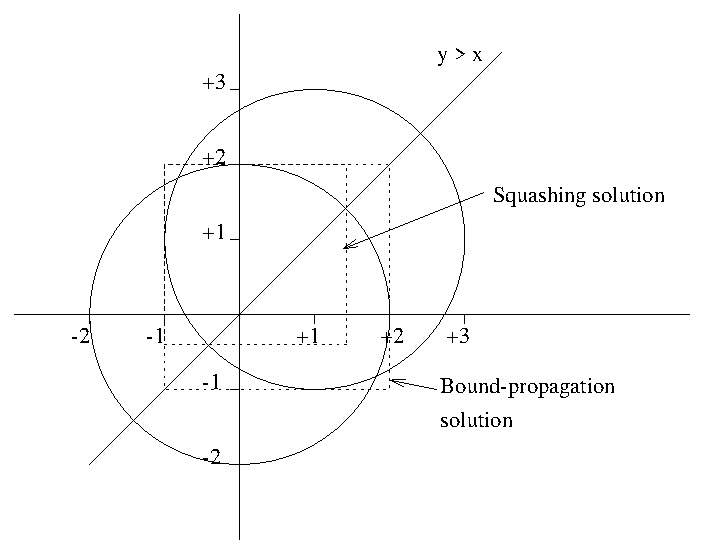
\includegraphics{example1.eps}
\caption{Propagation with Squash algorithm (example)}
\end{figure}

All points (X,Y) Y $>$= X, lying within the intersection of 2 circles with
radius 2, one centred at (0,0) the other at (1,1).
\begin{quote}
\begin{verbatim}
[eclipse 2]: 4 $>= X^2 + Y^2, 4 $>= (X-1)^2+(Y-1)^2, Y $>= X.

Y = Y{-1.0000000000000004 .. 2.0000000000000004}
X = X{-1.0000000000000004 .. 2.0000000000000004}

Delayed goals:
    ...
yes.
\end{verbatim}
\end{quote}
The bound-consistency solution does not take into account the X $>$= Y
constraint. Intuitively this is because it passes through the corners
of the box denoting the solution to the problem of simply intersecting
the two circles.

\begin{quote}
\begin{verbatim}
[eclipse 2]: 4 $>= X^2 + Y^2, 4 $>= (X-1)^2+(Y-1)^2, Y $>= X,
                squash([X,Y], 1e-5, lin).

X = X{-1.0000000000000004 .. 1.4142135999632601}
Y = Y{-0.41421359996326 .. 2.0000000000000004}

Delayed goals:
    ...
yes.
\end{verbatim}
\end{quote}

\subsection{Obtaining Solver Statistics}

(Using the facilities described in this section requires importing the
\bipref{ic_kernel}{../bips/lib/ic_kernel/index.html} module.  Also, since
they depend on the internals of the IC library, the details presented here
are subject to change without notice.)

Often it is difficult to know where the solver spends its time.
The library has built-in counters which keep track of the number of times
various events occur:
\begin{description}
    \item[ic_lin_create]
	The number of linear constraints set up.
    \item[ic_lin_prop]
	The number of times a linear constraint is propagated.
    \item[ic_uni_prop/ic_bin_prop/ic_tern_prop]
	The number of times a non-linear (unary/binary/ternary) operator is
	propagated.
    \item[ic_split]
	The number of domain splits in locate/2,3,4.
    \item[ic_squash]
	The number of squash attempts in squash/3 or locate/4.
\end{description}

Users who wish to track activity within their own programs may (if they
wish) use the same mechanism.  New event types can be registered (see
below) and actions recorded by calling the
\biptxtref{ic\_event(Event)}{ic_event/1!ic_kernel}{../bips/lib/ic_kernel/ic_event-1.html}
predicate.

The counters are controlled using the primitives:
\begin{description}
\item[\biptxtref{ic\_stat(on)}{ic_stat/1!ic_kernel}{../bips/lib/ic_kernel/ic_stat-1.html}]
\item[\biptxtref{ic\_stat(off)}{ic_stat/1!ic_kernel}{../bips/lib/ic_kernel/ic_stat-1.html}]
Enables/disable collection of statistics.  Default is off.

\item[\biptxtref{ic\_stat(reset)}{ic_stat/1!ic_kernel}{../bips/lib/ic_kernel/ic_stat-1.html}]
Reset statistics counters.

\item[\biptxtref{ic\_stat(print)}{ic_stat/1!ic_kernel}{../bips/lib/ic_kernel/ic_stat-1.html}]
Print statistics counters to the standard output stream.

\item[\biptxtref{ic\_stat_get(-Stat)}{ic_stat_get/1!ic_kernel}{../bips/lib/ic_kernel/ic_stat_get-1.html}]
Returns a list of CounterName=CounterValue pairs, summarising the
computation since the last reset.

\item[\biptxtref{ic\_event(+Name)}{ic_event/1!ic_kernel}{../bips/lib/ic_kernel/ic_event-1.html}]
Records the fact that the named event has happened.

\item[\biptxtref{ic_stat\_register\_event(+Name,+Description)}{ic_stat_register_event/2!ic_kernel}{../bips/lib/ic_kernel/ic_stat_register_event-2.html}]
Registers a new event type and sets the counter to 0.  This allows
user-defined predicates to record their own events within the same
framework.

\end{description}


\section{General Guidelines for the Use of the IC library}
Whilst IC has been designed to provide a flexible, consistent and yet
powerful framework for many sorts of constraint satisfaction
problems, it can not be all things to all people.

There are circumstances under which IC will not propagate all possible
information, for reasons of efficiency.

It is the purpose of this section to point out ways that may help IC
to solve problems more efficiently.

Typical constraint satisfaction problems are solved by iteratively
propagating information from basic constraints until no more
propagation can take place (i.e.\ a fixed point has been reached), and
then reducing the domain of a variable so as to prompt more
propagation.

As with most constraint solvers the propagation provided by the
builtin constraints is rarely able to solve large problems completely
without the need for some form of search.  A number of factors affect
the speed of the propagation phase.

\begin{enumerate}
\item The size of the initial domains.
Smaller domains typically result in propagation reaching a fixed point
sooner.  So give explicit initial domains to as many variables as possible.
\item Integer domains allow more propagation.
An important point to note here is that (as in mathematics) IC treats
integers as a strict subset of the reals, and as such the integer
domain \verb|0 .. 100| contains significantly fewer values than the
real domain \verb|0.0 .. 100.0|.  With this in mind, IC attempts to
infer integrality where possible (e.g.\ the sum of two integer variables
is constrained to be integer), however integer domains (where
applicable) should be used in user code.

The difference becomes apparent when dealing with strict inequalities, for example.
\begin{verbatim}
[eclipse 4]: reals([X]), X $> 5.

X = X{5.0 .. 1.0Inf}


Delayed goals:
        ic : (X{5.0 .. 1.0Inf} > 5)
Yes (0.00s cpu)
\end{verbatim}
Note that the lower bound of X is still five despite the fact that X
has been constrained to be strictly greater than five.  Further note
the presence of a delayed goal which will fail should X be constrained
to be exactly five.

\begin{verbatim}
[eclipse 5]: integers([X]), X $> 5.

X = X{6 .. 1.0Inf}
Yes (0.00s cpu)
\end{verbatim}
In this example since X is known to be integral, the lower bound of X
can be set to 6, as there are no integers between five and six.
\end{enumerate}


\section{User defined constraints}

The library \bipref{ic_kernel}{../bips/lib/ic_kernel/index.html} provides a
number of facilities useful for implementing IC constraints or otherwise
extending the facilities provided by the standard IC library.

While the \bipref{ic_kernel}{../bips/lib/ic_kernel/index.html} library
exposes the structure of the IC attribute to the programmer (see below),
accessing it directly is strongly discouraged (if for no other reason,
the internals of IC may continue to evolve).
For accessing information about a variable and its domain, use the
predicates described earlier in section~\ref{domain-query} ``Variable query
predicates''.
For modifying a variable, it is particularly important to go through the
access predicates, in order to make sure that the internal state remains
consistent, that appropriate constraints are scheduled for execution as a
result of the change, etc.
The predicates available for modifying a variable are discussed in the next
section.

\subsection{Modifying variable domains}

When using IC variables in normal code, one would typically use the
\verb|$\=|, \verb|$=<| and \verb|$>=| family of constraints to (resp.)
remove a value, reduce the upper bound or increase the lower bound of a
variable.

While these constraints are good for normal CSP solving, they have a
number of properties which may be less desirable when writing new
constraints.  In particular, they may leave unwanted delayed goals
behind and may perform extra propagation before returning (it may be
desirable to perform all required bound updates before allowing further
propagation to occur).

To give the constraint writer more control over such matters, special
predicates exist in the \bipref{ic_kernel}{../bips/lib/ic_kernel/index.html}
module which allow direct modification of the domain without the waking of
goals (they are scheduled for execution but not actually executed).
These predicates generally accept an IC variable, a non-IC variable (which
will be constrained to make it a real IC variable) or a number.

Full details on these predicates can be found in the reference manual; they
are listed here for completeness.  Note that with the exception of
\bipref{impose_bounds/3}{../bips/lib/ic_kernel/impose_bounds-3.html} none of
the goals call \bipref{wake/0}{../bips/kernel/suspensions/wake-0.html}, so
the programmer is free to do so at a convenient time.

\begin{description}
\item[\bipref{impose_min/2}{../bips/lib/ic_kernel/impose_min-2.html}]
Set the lowerbound.
\item[\bipref{impose_max/2}{../bips/lib/ic_kernel/impose_max-2.html}]
Set the upperbound.
\item[\bipref{impose_bounds/3}{../bips/lib/ic_kernel/impose_bounds-3.html}]
Sets both upper and lower bounds.
\item[\bipref{exclude/2}{../bips/lib/ic_kernel/exclude-2.html}]
Excludes an integer from an integral variable.
\item[\bipref{exclude_range/3}{../bips/lib/ic_kernel/exclude_range-3.html}]
Excludes a range of integers from an integral variable.
\item[\bipref{set_var_type/2}{../bips/lib/ic_kernel/set_var_type-2.html}]
Makes the variable be of the given type.
\item[\bipref{set_vars_type/2}{../bips/lib/ic_kernel/set_vars_type-2.html}]
Like set_var_type, but works for lists and submatrices of variables as well.
\end{description}

\subsection{The IC attribute}

The IC attribute is a meta-term which is attached to all variables which
take part in IC constraints.
\bipref{ic_kernel}{../bips/lib/ic_kernel/index.html} defines the IC
attribute as a structure of the following form:
\begin{verbatim}
ic{var_type:Type,
         lo:Lo,
         hi:Hi,
         bitmap:Bitmap,
         min:SuspMin,
         max:SuspMax,
         hole:SuspHole,
         type:SuspType
        }
\end{verbatim}


This structure holds:

\begin{description}
\item[var_type] The type of the variable.  This defaults to 'real' but may
become 'integer' after an explicit call to {\bf integers/1}, by being
included in an integer constraint (e.g.\ {\bf \#=}) or by inferences made
during constraint propagation.
\item[lo] The lower bound of the variable's domain, as a float.
\item[hi] The lower bound of the variable's domain, as a float.
\item[bitmap] Where relevant, a bitmap representation of the integer domain;
where not relevant it holds the atom \verb|undefined|.
\item[min] Suspension list of goals to be woken on lower bound changes.
\item[max] Suspension list of goals to be woken on upper bound changes.
\item[hole] Suspension list of goals to be woken when a value is removed
from the middle of a domain.  Such removals only happen for integer
variables whose domain is finite.
\item[type] Suspension list of goals to be woken when a variable's type
becomes more constrained, i.e.\ when a variable goes from being real to
being integer.
\end{description}

The suspension list names can be used in
\bipref{suspend/3}{../bips/kernel/suspensions/suspend-3.html} and
related predicates to denote an appropriate waking condition.

The attribute of a domain variable can be accessed with the predicate
\bipref{get_ic_attr/2}{../bips/lib/ic_kernel/get_ic_attr-2.html}.

As noted above, direct access and manipulation of the attribute is
discouraged; use the access predicates instead.

\index{library!ic|)}

%HEVEA\cutend



% BEGIN LICENSE BLOCK
% Version: CMPL 1.1
%
% The contents of this file are subject to the Cisco-style Mozilla Public
% License Version 1.1 (the "License"); you may not use this file except
% in compliance with the License.  You may obtain a copy of the License
% at www.eclipse-clp.org/license.
% 
% Software distributed under the License is distributed on an "AS IS"
% basis, WITHOUT WARRANTY OF ANY KIND, either express or implied.  See
% the License for the specific language governing rights and limitations
% under the License. 
% 
% The Original Code is  The ECLiPSe Constraint Logic Programming System. 
% The Initial Developer of the Original Code is  Cisco Systems, Inc. 
% Portions created by the Initial Developer are
% Copyright (C) 2006 Cisco Systems, Inc.  All Rights Reserved.
% 
% Contributor(s): Joachim Schimpf, IC-Parc
% 
% END LICENSE BLOCK
%
% $Id: fdglobal.tex,v 1.2 2013/02/09 14:59:59 jschimpf Exp $
%
% Author: Joachim Schimpf
%

\chapter{Global Finite Domain Constraints}
\label{chapglobconstr}
%HEVEA\cutdef[1]{section}
\section{Various Constraints over Lists and Arrays}

The libraries
\biptxtref{ic_global}{library(ic_global)}{../bips/lib/ic_global/index.html}
and
\biptxtref{ic_global_gac}{library(ic_global_gac)}{../bips/lib/ic_global_gac/index.html}
implement a number of constraints over lists of integer variables.
They are loaded using a directive like
\begin{quote}\begin{verbatim}
:- use_module(library(ic_global)).	% or :- lib(ic_global).
\end{verbatim}\end{quote}
For details of the implemented constraints, refer to the Reference Manual
for the libraries.

These constraints are commonly known as \aboutidx{global constraints},
which simply indicates that they can constrain a large number of variables
at once, without breaking up the constraint into more primitive constraints.
This can on one hand facilitate problem modelling, and on the other hand
lead to more effective constraint propagation.

Note that some constraints are implemented in both of the libraries:
in these cases, ic_global_gac implements a "globally arc consistent"
version, while ic_global implements a less computationally expensive
version with weaker propagation.

Among the constraints provided are the following (refer to the
Reference Manual for the complete list):

\begin{description}
\item[\biptxtref{alldifferent(+List)}{ic_global:alldifferent/1}{../bips/lib/ic_global/alldifferent-1.html}]\ \\
\index{alldifferent/1}
A version of alldifferent/1 with strong propagation.

\item[\biptxtref{alldifferent(+List, ++Capacity)}{ic_global:alldifferent/2}{../bips/lib/ic_global/alldifferent-2.html}]\ \\
\index{alldifferent/2}
Like alldifferent/1, but every value may occur Capacity times.

\item[\biptxtref{alldifferent_matrix(+Matrix)}{alldifferent_matrix/1}{../bips/lib/ic_global_gac/alldifferent_matrix-1.html}]\ \\
Constrains the rows and columns of Matrix to be different values.

\item[\biptxtref{gcc(++Bounds,+Vars)}{gcc/2}{../bips/lib/ic_global_gac/gcc-2.html}]\ \\
The \aboutidx{global cardinality constraint} makes sure certain values
occur with a certain frequency in Vars.  This is a generalisation of the
occurrences-constraint.
See also \bipref{gcc_matrix/3}{../bips/lib/ic_global_gac/gcc_matrix-3.html}.

\item[\biptxtref{inverse(+Succ, +Pred)}{inverse/2}{../bips/lib/ic_global_gac/inverse-2.html}]\ \\
Constrains elements of Succ to be the successors and Pred to be the
predecessors of nodes in a digraph.

\item[\biptxtref{lex_le(+List1, +List2)}{lex_le/2}{../bips/lib/ic_global/lex_le-2.html}]\ \\
\index{lexico_le/2}
Imposes a lexicographic ordering between the two lists.

\item[\biptxtref{lex_lt(+List1, +List2)}{lex_lt/2}{../bips/lib/ic_global/lex_lt-2.html}]\ \\
Imposes a strict lexicographic ordering between the two lists.

\item[\biptxtref{ordered(++Relation, +List)}{ordered/2}{../bips/lib/ic_global/ordered-2.html}]\ \\
\index{ordered/2}
Constrains List to be ordered according to Relation.
Relation is one of the atoms \lt, =\lt, \gt, \gt=, = .

\item[\biptxtref{ordered_sum(++List, +Sum)}{ordered_sum/2}{../bips/lib/ic_global/ordered_sum-2.html}]\ \\
\index{ordered_sum/2}
The list elements are ordered and their sum is Sum.  A combination of
ordered and sum constraint with stronger propagation.

\item[\biptxtref{occurrences(++Value, +List, ?N)}{occurrences/3}{../bips/lib/ic_global/occurrences-3.html}]\ \\
\index{occurrences/3}
The value Value occurs in List N times.
Operationally: N gets updated to reflect the number of
possible occurrences in the List. List elements may get
instantiated to Value, or Value may be removed from their
domain if required by N.

\item[\biptxtref{same(+List1, +List2)}{same/2}{../bips/lib/ic_global_gac/same-2.html}]\ \\
List2 is a permutation of List1.

\item[\biptxtref{sequence(+Low, +High, +K, +Vars, ++Values)}{sequence/5}{../bips/lib/ic_global_gac/sequence-5.html}]\ \\
Every subsequence of Vars of length K contains at least Low and at most High
occurrences of Values.
Also \bipref{sequence/4}{../bips/lib/ic_global_gac/sequence-4.html}.

\item[\biptxtref{sorted(?List, ?Sorted)}{ic_global:sorted/2}{../bips/lib/ic_global/sorted-2.html}]\ \\
\index{sorted/2}
Sorted is a sorted permutation of List.

\item[\biptxtref{sorted(?List, ?Sorted, ?Positions)}{ic_global:sorted/3}{../bips/lib/ic_global/sorted-3.html}]\ \\
\index{sorted/3}
Sorted is a sorted permutation of List and Positions is a list whose
elements indicating the position of each unsorted list element within
the sorted list.

\item[\biptxtref{sumlist(+List, ?Sum)}{ic_global:sumlist/2}{../bips/lib/ic_global/sumlist-2.html}]\ \\
\index{sumlist/2}
The sum of the list elements is Sum. This constraint
is more efficient than a general IC sum constraint
if the list is long and Sum is not constrained frequently.

\end{description}


\section{Cumulative Constraint and Resource Profiles}

The library {\bf cumulative} implements the cumulative scheduling constraint.
It is based on the IC library and is loaded using one of 
\begin{quote}\begin{verbatim}
:- use_module(library(ic_cumulative)).
:- lib(ic_cumulative).
\end{verbatim}\end{quote}


\begin{description}
\item[\biptxtref{cumulative(+StartTimes, +Durations, +Resources, ++ResourceLimit)}{ic_cumulative:cumulative/4}{../bips/lib/ic_cumulative/cumulative-4.html}]\ \\
\index{cumulative/4}
A cumulative scheduling constraint. StartTimes, Durations and Resources
are lists of equal length N of integer variables or integers.
ResourceLimit is an integer. The declarative meaning is:
If there are N tasks, each starting at a certain start time, having
a certain duration and consuming a certain (constant) amount of
resource, then the sum of resource usage of all the tasks does not
exceed ResourceLimit at any time.

\item[\biptxtref{profile(+StartTimes, +Durations, +Resources, -Profile)}{ic_cumulative:profile/4}{../bips/lib/ic_cumulative/profile-4.html}]\ \\
\index{profile/4}
StartTimes, Durations, Resources and Profile
are lists of equal length N of integer variables or integers
with the same meaning as in cumulative/4.
The list Profile indicates the level of resource usage at the
starting point of each task.
\end{description}


\section{Edge-finder}

The libraries {\bf ic_edge_finder} and {\bf ic_edge_finder3}
implement stronger versions of the
disjunctive and cumulative scheduling constraints. They employ
a technique known as edge-finding to derive stronger bounds on
the starting times of the tasks.
The library is loaded using either
\begin{quote}\begin{verbatim}
:- use_module(library(ic_edge_finder)).
\end{verbatim}\end{quote}
to get a weaker variant with quadratic complexity, or
\begin{quote}\begin{verbatim}
:- use_module(library(ic_edge_finder3)).
\end{verbatim}\end{quote}
to get a stronger variant with cubic complexity.

\begin{description}
\item[disjunctive(+StartTimes,+Durations)]\ \\
\index{disjunctive/2}
A disjunctive scheduling constraint. StartTimes and Durations
are lists of equal length N of integer variables or integers.
The declarative meaning is that the N tasks with certain start times
and duration do not overlap at any point in time.

\item[cumulative(+StartTimes,+Durations,+Resources,++ResourceLimit)]\ \\
\index{cumulative/4}
A cumulative scheduling constraint. StartTimes, Durations and Resources
are lists of equal length N of integer variables or integers.
ResourceLimit is an integer. The declarative meaning is:
If there are N tasks, each starting at a certain start time, having
a certain duration and consuming a certain (constant) amount of
resource, then the sum of resource usage of all the tasks does not
exceed ResourceLimit at any time.
This constraint can propagate more information than the implementation
in library(cumulative).

\item[cumulative(+StartTimes,+Durations,+Resources,+Area,++ResourceLimit)]\ \\
\index{cumulative/5}
In this variant, an area (the product of duration and resource usage of
a task) can be specified, e.g.\ if duration or resource usage are not
known in advance. The edge-finder algorithm can make use of this information
to derive bound updates.
\end{description}
%HEVEA\cutend

% BEGIN LICENSE BLOCK
% Version: CMPL 1.1
%
% The contents of this file are subject to the Cisco-style Mozilla Public
% License Version 1.1 (the "License"); you may not use this file except
% in compliance with the License.  You may obtain a copy of the License
% at www.eclipse-clp.org/license.
% 
% Software distributed under the License is distributed on an "AS IS"
% basis, WITHOUT WARRANTY OF ANY KIND, either express or implied.  See
% the License for the specific language governing rights and limitations
% under the License. 
% 
% The Original Code is  The ECLiPSe Constraint Logic Programming System. 
% The Initial Developer of the Original Code is  Cisco Systems, Inc. 
% Portions created by the Initial Developer are
% Copyright (C) 2006 Cisco Systems, Inc.  All Rights Reserved.
% 
% Contributor(s): 
% 
% END LICENSE BLOCK

%----------------------------------------------------------------------
\chapter{The Integer Sets Library}
%HEVEA\cutdef[1]{section}
\label{chapfdsets}
\index{library!fd_sets|(}
%----------------------------------------------------------------------


%----------------------------------------------------------------------
%\section{Introduction}
%----------------------------------------------------------------------

The {\em fd_sets} library is a solver for constraints over the domain
of finite sets of integers. Unlike {\em conjunto}, it cannot deal with
sets elements that are not integers. On the other hand, fd_sets is usually
faster for integer sets than conjunto.



\section{Ground Integer Sets}

(Ground) integer sets are simply sorted, duplicate-free lists of integers e.g. 
\begin{verbatim}
        SetOfThree = [1,3,7]
        EmptySet = []
\end{verbatim}
Lists which contain non-integers, are unsorted or contain duplicates,
are not sets in the sense of this library.


%----------------------------------------------------------------------
\section{Set Variables}
%----------------------------------------------------------------------

\subsection{Declaring}
Set variables are variables which can eventually take a ground integer
set as their value.  They are characterized by a lower bound (the set
of elements that are definitely in the set) and an upper bound (the
set of elements that may be in the set).  A set variable can be
declared as follows: 
\begin{verbatim}
        SetVar :: []..[1,2,3,4,5,6,7]
\end{verbatim}
If the lower bound is the empty set (like in this case) this can be written as 
\begin{verbatim}
        SetVar subset [1,2,3,4,5,6,7]
\end{verbatim}
If the lower bound is the empty set and the upper bound is a set of
consecutive integers, one can also declare it like
\begin{verbatim}
        intset(SetVar, 1, 7)
\end{verbatim}
which is equivalent to the above.    

The predicates to declare sets are:
\begin{description}
\item[\biptxtref{?Set :: ++Lwb..++Upb}{::/2!fd_sets}{../bips/lib/fd_sets/NN-2.html}]
         Set is an integer set within the given bounds 
\item[\biptxtref{intset(?Set, +Min, +Max)}{intset/3}{../bips/lib/fd_sets/intset-3.html}]
         Set is a set containing numbers between Min and Max 
\item[\biptxtref{intsets(?Sets, ?N, +Min, +Max)}{intsets/4}{../bips/lib/fd_sets/intsets-4.html}]
         Sets is a list of N sets containing numbers between Min and Max 
\end{description}



\subsection{Printing}

Set variables are by default printed in a particular way, e.g.
\begin{verbatim}
?- X :: [2,3]..[1,2,3,4], write(X).
X{[2, 3] \/ ([] .. [1, 4]) : _308{[2 .. 4]}}
\end{verbatim}
The curly brackets contain
\begin{enumerate}
\item the lower bound of the set
\item the union symbol
\item the set of optional values (that may or may not be in the set)
\item a colon
\item a finite domain indicating the admissible cardinality for the set
\end{enumerate}



\subsection{Domain Access}

\begin{description}
\item[\biptxtref{potential_members(?Set, -List)}{potential_members/2}{../bips/lib/fd_sets/potential_members-2.html}]
         List is the list of elements of whose membership in Set is currently uncertain 
\item[\biptxtref{set_range(?Set, -Lwb, -Upb)}{set_range/3}{../bips/lib/fd_sets/set_range-3.html}]
         Lwb and Upb are the current lower and upper bounds on Set 
\end{description}


%----------------------------------------------------------------------
\section{Constraints}
%----------------------------------------------------------------------

\subsection{Membership}

\begin{description}
\item[\biptxtref{?X in ?Set}{in/2!fd_sets}{../bips/lib/fd_sets/in-2.html}]
         The integer X is member of the integer set Set 
\item[\biptxtref{?X notin ?Set}{notin/2!fd_sets}{../bips/lib/fd_sets/notin-2.html}]
         The integer X is not a member of the integer set Set 
\item[\biptxtref{membership_booleans(?Set, ?BoolArr)}{membership_booleans/2!fd_sets}{../bips/lib/fd_sets/membership_booleans-2.html}]
         BoolArr is an array of booleans describing Set 
\end{description}


\subsection{Cardinality}

\begin{description}
\item[\biptxtref{\#(?Set, ?Card)}{\#/2!fd_sets}{../bips/lib/fd_sets/H-2.html}]
         Card is the cardinality of the integer set Set 
\end{description}


\subsection{Set Relations}

\begin{description}

\item[\biptxtref{difference(?Set1, ?Set2, ?Set3)}{difference/3!fd_sets}{../bips/lib/fd_sets/difference-3.html}]
         Set3 is the difference of the integer sets Set1 and Set2 

\item[\biptxtref{?Set1 disjoint ?Set2}{disjoint/2!fd_sets}{../bips/lib/fd_sets/disjoint-2.html}]
         The integer sets Set1 and Set2 are disjoint 

\item[\biptxtref{?Set1 includes ?Set2}{includes/2!fd_sets}{../bips/lib/fd_sets/includes-2.html}]
         Set1 includes (is a superset) of the integer set Set2 

\item[\biptxtref{intersection(?Set1, ?Set2, ?Set3)}{intersection/3!fd_sets}{../bips/lib/fd_sets/intersection-3.html}]
         Set3 is the intersection of the integer sets Set1 and Set2 

\item[\biptxtref{?Set1 sameset ?Set2}{sameset/2!fd_sets}{../bips/lib/fd_sets/sameset-2.html}]
         The sets Set1 and Set2 are equal 
\item[\biptxtref{?Set1 subset ?Set2}{subset/2!fd_sets}{../bips/lib/fd_sets/subset-2.html}]
         Set1 is a subset of the integer set Set2 
\item[\biptxtref{symdiff(?Set1, ?Set2, ?Set3)}{symdiff/3!fd_sets}{../bips/lib/fd_sets/symdiff-3.html}]
         Set3 is the symmetric difference of the integer sets Set1 and Set2 
\item[\biptxtref{union(?Set1, ?Set2, ?Set3)}{union/3!fd_sets}{../bips/lib/fd_sets/union-3.html}]
         Set3 is the union of the integer sets Set1 and Set2 
\end{description}


\subsection{N-ary Set Relations}

\begin{description}
\item[\biptxtref{all_disjoint(+Sets)}{all_disjoint/1}{../bips/lib/fd_sets/all_disjoint-1.html}]
         Sets is a list of integers sets which are all disjoint 
\item[\biptxtref{all_union(+Sets, ?SetUnion)}{all_union/2}{../bips/lib/fd_sets/all_union-2.html}]
         SetUnion is the union of all the sets in the list Sets 
\item[\biptxtref{all_intersection(+Sets, ?SetIntersection)}{all_intersection/2}{../bips/lib/fd_sets/all_intersection-2.html}]
         SetIntersection is the intersection of all the sets in the list Sets 
\end{description}


\subsection{Set Weights}

\begin{description}
\item[\biptxtref{weight(?Set, ++ElementWeights, ?Weight)}{weight/3}{../bips/lib/fd_sets/weight-3.html}]
         According to the array of element weights, the weight of set Set1 is Weight 
\end{description}


%----------------------------------------------------------------------
\section{Set Expressions}
%----------------------------------------------------------------------

In most positions where a set or set variable is expected one can also
use a set expression. A set expression is composed from ground sets
(integer lists), set variables, and the following set operators:
\begin{verbatim}
    Set1 /\ Set2       % intersection
    Set1 \/ Set2       % union
    Set1 \ Set2        % difference
\end{verbatim}
When such set expressions occur, they are translated into auxiliary
\bipref{intersection/3}{../bips/lib/fd_sets/intersection-3.html},
\bipref{union/3}{../bips/lib/fd_sets/union-3.html} and
\bipref{difference/3}{../bips/lib/fd_sets/difference-3.html}
constraints, respectively.


%----------------------------------------------------------------------
\section{Search Support}
%----------------------------------------------------------------------

The
\bipref{insetdomain/4}{../bips/lib/fd_sets/insetdomain-4.html}
predicate can be used to enumerate all ground instantiations of a set
variable, much like
\bipref{indomain/1}{../bips/lib/fd/indomain-1.html}
in the finite-domain case. 

\begin{description}
\item[\biptxtref{insetdomain(?Set, ?CardSel, ?ElemSel, ?Order)}{insetdomain/4}{../bips/lib/fd_sets/insetdomain-4.html}]
         Instantiate Set to a possible value 
\end{description}


%----------------------------------------------------------------------
\section{Example}
%----------------------------------------------------------------------

The following program computes so-called Steiner triplets.
These are triplets of numbers from 1 to N such that
any two triplets have at most one element in common.
\begin{verbatim}
:- lib(fd_sets).
:- lib(fd).

steiner(N, Sets) :-
        NB is N * (N-1) // 6,           % compute number of triplets
        intsets(Sets, NB, 1, N),        % initialise the set variables
        ( foreach(S,Sets) do
            #(S,3)                      % constrain their cardinality
        ),
        ( fromto(Sets,[S1|Ss],Ss,[]) do
            ( foreach(S2,Ss), param(S1) do
                #(S1 /\ S2, C),         % constrain the cardinality
                C #<= 1                 % of pairwise intersections
            )
        ),
        label_sets(Sets).               % search

label_sets([]).
label_sets([S|Ss]) :-
        insetdomain(S,_,_,_),
        label_sets(Ss).
\end{verbatim}
Here is an example of running this program
\begin{verbatim}
?- steiner(9,X).

X = [[1, 2, 3], [1, 4, 5], [1, 6, 7], [1, 8, 9],
     [2, 4, 6], [2, 5, 8], [2, 7, 9], [3, 4, 9],
     [3, 5, 7], [3, 6, 8], [4, 7, 8], [5, 6, 9]] More? (;)
\end{verbatim}

\index{library!fd_sets|)}

%HEVEA\cutend

% BEGIN LICENSE BLOCK
% Version: CMPL 1.1
%
% The contents of this file are subject to the Cisco-style Mozilla Public
% License Version 1.1 (the "License"); you may not use this file except
% in compliance with the License.  You may obtain a copy of the License
% at www.eclipse-clp.org/license.
% 
% Software distributed under the License is distributed on an "AS IS"
% basis, WITHOUT WARRANTY OF ANY KIND, either express or implied.  See
% the License for the specific language governing rights and limitations
% under the License. 
% 
% The Original Code is  The ECLiPSe Constraint Logic Programming System. 
% The Initial Developer of the Original Code is  Cisco Systems, Inc. 
% Portions created by the Initial Developer are
% Copyright (C) 2006 Cisco Systems, Inc.  All Rights Reserved.
% 
% Contributor(s): 
% 
% END LICENSE BLOCK

%----------------------------------------------------------------------
\chapter{The Symbolic Domain Library}
%HEVEA\cutdef[1]{section}
\label{chapicsymbolic}
\index{library!ic_symbolic|(}
%----------------------------------------------------------------------


%----------------------------------------------------------------------
%\section{Introduction}
%----------------------------------------------------------------------

The {\em ic_symbolic} library is a solver for constraints over ordered
symbolic domains.
It is implemented on top of library(ic) (see \ref{chapic}),
by mapping symbolic domains to finite integer domains.
There are also several mixed-domain constraints, which have both
symbolic and integer arguments.

%----------------------------------------------------------------------
\section{Domains and Domain Variables}
%----------------------------------------------------------------------

This library uses the
\biptxtref{domain}{domain/1}{../bips/kernel/termcomp/domain-1.html}
feature provided by the ECLiPSe kernel. 
This means that domains need to be declared.
The declaration specifies the domain values and their order. For example:
\begin{quote}\begin{verbatim}
?- local domain(weekday(mo,tu,we,th,fr,sa,su)).
\end{verbatim}\end{quote}
declares a domain with name 'weekday' and values 'mo', 'tu' etc.  The
domain values are implicitly ordered, with 'mo' corresponding to 1,
until 'su' corresponding to 7.  Domain values must be unique within
one ECLiPSe module, i.e. a symbolic value can belong to at most one
domain.

A variable of a declared domain can then be created using
\begin{quote}\begin{verbatim}
?- X &:: weekday.
X = X{[mo, tu, we, th, fr, sa, su]}
Yes (0.00s cpu)
\end{verbatim}\end{quote}
or multiple variables using
\begin{quote}\begin{verbatim}
?- [X,Y,Z] &:: weekday.
X = X{[mo, tu, we, th, fr, sa, su]}
Y = Y{[mo, tu, we, th, fr, sa, su]}
Z = Z{[mo, tu, we, th, fr, sa, su]}
Yes (0.00s cpu)
\end{verbatim}\end{quote}


%----------------------------------------------------------------------
\section{Basic Constraints}
%----------------------------------------------------------------------
The following constraints implement the basic relationships between
two domain values.  The constraints require their arguments to come
from identical domains, otherwise an error is raised.
\begin{description}
\item[\biptxtref{?X \&= ?Y}{\&=/2!ic_symbolic}{../bips/lib/ic_symbolic/YE-2.html}]
    X is the same as Y
\item[\biprefnoidx{?X \&\bsl= ?Y}{../bips/lib/ic_symbolic/YRE-2.html}]
    \index{\&\bsl=/2!ic_symbolic}
    X is different from Y
\item[\biptxtref{?X \&$>$ ?Y}{\&</2!ic_symbolic}{../bips/lib/ic_symbolic/YL-2.html}]
    X is strictly before Y in the domain order
\item[\biptxtref{?X \&$<$ ?Y}{\&>/2!ic_symbolic}{../bips/lib/ic_symbolic/YG-2.html}]
    X is strictly after Y in the domain order
\item[\biptxtref{?X \&=$<$ ?Y}{\&=</2!ic_symbolic}{../bips/lib/ic_symbolic/YEL-2.html}]
    X is the same as Y, or before Y in the domain order
\item[\biptxtref{?X \&$>$= ?Y}{\&>=/2!ic_symbolic}{../bips/lib/ic_symbolic/YGE-2.html}]
    X is the same as Y, or after Y in the domain order
\item[\biptxtref{shift(?X,?C,?Y)}{shift/1!ic_symbolic}{../bips/lib/ic_symbolic/shift-3.html}]
    Y is C places above X in the domain order.
    X and Y have symbolic domains, C has an integer domain.
\item[\biptxtref{rotate(?X,?C,?Y)}{rotate/3!ic_symbolic}{../bips/lib/ic_symbolic/rotate-3.html}]
    like shift/3 but wraps at domain boundary.
\item[\biptxtref{element(?Index,++List,?Value)}{element/3!ic_symbolic}{../bips/lib/ic_symbolic/element-3.html}]
    Value occurs List at position Index.
    Value has a symbolic domain, Index has an integer domain.
    List is a number of symbolic domain values.
\end{description}
For example
\begin{quote}\begin{verbatim}
?- [X, Y] &:: weekday, X &< Y.
X = X{[mo, tu, we, th, fr, sa]}
Y = Y{[tu, we, th, fr, sa, su]}
Yes (0.00s cpu)

?- X &:: weekday, X &=< we.
X = X{[mo, tu, we]}
Yes (0.00s cpu)
\end{verbatim}\end{quote}
    

%----------------------------------------------------------------------
\section{Global Constraints}
%----------------------------------------------------------------------
A number of global constraints are available which directly correspond
(and are in fact implemented via) their counterparts in
lib(ic_global):
\begin{description}
\item[\biptxtref{alldifferent(+List)}{alldifferent/1!ic_symbolic}{../bips/lib/ic_symbolic/alldifferent-1.html}]
    All list elements are different
\item[\biptxtref{occurrences(++Value,+List,?N)}{occurrences/3!ic_symbolic}{../bips/lib/ic_symbolic/occurrences-3.html}]
    Value occurs N times in List
\item[\biptxtref{atmost(++N,+List,++Value)}{atmost/3!ic_symbolic}{../bips/lib/ic_symbolic/atmost-3.html}]
    Value occurs at most N times in List
\end{description}


%----------------------------------------------------------------------
\section{Internals}
%----------------------------------------------------------------------

Internally, symbolic domains are mapped to integer ranges from 1 up to
the number of domain elements.  The first value in the domain
declaration corresponds to 1, the second to 2 and so on.  Similarly,
symbolic domain variables can be mapped to a corresponding IC integer
variable.  This mapping is accessible through the predicate
\bipref{symbol_domain_index/3}{../bips/lib/ic_symbolic/symbol_domain_index-3.html}:
\begin{quote}\begin{verbatim}
?- symbol_domain_index(fr, D, I).
D = weekday
I = 5
Yes (0.00s cpu)

?- X &:: weekday, symbol_domain_index(X, D, I).
X = X{[mo, tu, we, th, fr, sa, su]}
D = weekday
I = I{1 .. 7}
Yes (0.00s cpu)

?- X &:: weekday, X &\= we, symbol_domain_index(X, D, I).
X = X{[mo, tu, th, fr, sa, su]}
D = weekday
I = I{[1, 2, 4 .. 7]}
Yes (0.00s cpu)
\end{verbatim}\end{quote}
    
The integer variable I mirrors the domain of the symbolic variable X and vice versa.

%----------------------------------------------------------------------
\section{Extending and Interfacing this Library}
%----------------------------------------------------------------------

Because of the mapping of symbols to integers, new constraints over
symbolic variables can be implemented simply by placing numeric (IC)
constraints on the corresponding integer variables.

Similarly, the facilities of the ic_search library can be exploited
when working with symbolic variables.  Instead of labeling the
symbolic variables, one can use the various facilities of ic_search to
label the corresponding integer variables instead.


%----------------------------------------------------------------------
\index{library!ic_symbolic|)}
%----------------------------------------------------------------------

%HEVEA\cutend

\chapter{GFD: Interface to Gecode Finite Domain Solver}
\label{chapgfd}
LIBRARY		"gfd.dll"
DESCRIPTION	"ECLiPSe Gecode Interface"
EXPORTS
	p_g_init			@1
        p_g_state_is_stable		@2
        p_g_check_handle		@3
        p_g_trail_undo_for_event	@4
        p_g_delete			@5
        p_g_add_newbool			@6
        p_g_add_newvars_interval	@7
        p_g_add_newvars_dom		@8
	p_g_add_newvars_as_bool		@9
        p_g_post_interval		@10
        p_g_post_var_interval_reif	@11
        p_g_post_dom			@12
        p_g_post_var_dom_reif		@13
        p_g_post_var_val_reif		@14
        p_g_post_setvar			@15
        p_g_post_intrel_cstr		@16
        p_g_post_bool_connectives	@17
        p_g_post_alldiff		@18
        p_g_post_alldiff_offsets	@19
        p_g_post_count			@20
        p_g_post_gcc			@21
        p_g_post_element		@22
        p_g_post_sorted2		@23
        p_g_post_sorted			@24
        p_g_post_sequence		@25
        p_g_post_sequence_01		@26
        p_g_post_circuit		@27
        p_g_post_circuit_cost		@28
        p_g_post_disj			@29
        p_g_post_disjflex		@30
        p_g_post_cumulative		@31
        p_g_post_cumulativeflex		@32
        p_g_post_cumulatives		@33
	p_g_post_ordered		@34
	p_g_post_lex_order		@35
	p_post_bin_packing		@36	
        p_g_post_sum			@37
        p_g_post_lin			@38
        p_g_post_sum_reif		@39
        p_g_post_lin_reif		@40
        p_g_post_maxlist		@41
        p_g_post_minlist		@42
        p_g_post_sqrt			@43
        p_g_post_sq			@44
        p_g_post_abs			@45
        p_g_post_div			@46
        p_g_post_mult			@47
        p_g_post_mod			@48
        p_g_post_min2			@49
        p_g_post_max2			@50
        p_g_post_divmod			@51
        p_g_post_boolchannel		@52
        p_g_post_inverse		@53
        p_g_post_inverse_offset		@54
	p_g_post_ordered		@55
	p_g_post_lex_order		@56
        p_g_post_bin_packing		@57
        p_g_post_cumulative		@58
        p_g_propagate			@59
        p_g_check_val_is_in_var_domain	@60
        p_g_get_var_bounds		@61
        p_g_get_var_value		@62
        p_g_get_var_domain		@63
        p_g_get_var_lwb			@64
        p_g_update_and_get_var_bound	@65
        p_g_get_var_upb			@66
        p_g_get_var_domain_size		@67
        p_g_get_var_domain_width	@68
        p_g_get_var_degree		@69
        p_g_get_var_median		@70
        p_g_get_var_afc			@71
        p_g_get_var_regret_lwb		@72
        p_g_get_var_regret_upb		@73
        p_g_setup_search		@74
        p_g_do_search			@75
        p_g_get_gfd_maxint		@76
        p_g_get_gfd_minint		@77
        p_g_add_newvars_dom_union	@78
        p_g_get_var_domain_handle	@79
        p_g_add_newvar_copy		@80
	p_g_link_newbools		@81
	p_g_gecode_version		@82


% BEGIN LICENSE BLOCK
% Version: CMPL 1.1
%
% The contents of this file are subject to the Cisco-style Mozilla Public
% License Version 1.1 (the "License"); you may not use this file except
% in compliance with the License.  You may obtain a copy of the License
% at www.eclipse-clp.org/license.
% 
% Software distributed under the License is distributed on an "AS IS"
% basis, WITHOUT WARRANTY OF ANY KIND, either express or implied.  See
% the License for the specific language governing rights and limitations
% under the License. 
% 
% The Original Code is  The ECLiPSe Constraint Logic Programming System. 
% The Initial Developer of the Original Code is  Cisco Systems, Inc. 
% Portions created by the Initial Developer are
% Copyright (C) 1999 - 2006 Cisco Systems, Inc.  All Rights Reserved.
% 
% Contributor(s): Mark Wallace, IC-Parc
% 
% END LICENSE BLOCK

%
% @(#)extpropia.tex	2.0 23/02/99 
%
% Author: Mark Wallace
%
%\documentstyle{report}
%\begin{document}
\chapter{Propia - A Library Supporting Generalised Propagation}
%HEVEA\cutdef[1]{section}
\label{chappropia}

\label{Propia}
\index{Propia}
\section{Overview}

Propia is the name for the implementation of Generalised Propagation in
\eclipse.
  
Generalised propagation is {\em not} restricted
to integer domains, but can be applied to any goal the user cares to specify
even if the variables don't have domains.

Effectively the system looks ahead to determine if 
an approximation to the possible answers has a non-trivial generalization.
It is non-trivial if it enables any variables in the goal to become
further instantiated, thus reducing search.  

The background and motivation for Generalised Propagation is given in
references \cite{LeProvost92,LeProvost92a,LeProvost93b}.  This section
focusses on how to use it.  Further examples of the use of Propia are
distributed with \eclipse in the \verb+doc/examples/propia/+ directory
.  A simple demonstration of Propia in action on Lewis Carroll's Zebra
problem can be run by compiling \verb0zebra.pl0 and issuing the query
\verb+lib(ic), zebra(Houses,ic)+ .  An slightly more complex
application of Propia to crossword generation can be run by compiling
\verb0crossword0.


\index{infers}
Using Propia it is easy to take a standard Prolog program and, with
minimal syntactic change, to turn it into a constraint logic program.
Any goal \verb0Goal0 in the Prolog program, can be transformed into a
constraint by annotating it thus \verb0Goal infers most0.
The resulting constraint admits just the same answers as
the original goal, but its behaviour is quite different.
Instead of evaluating the goal by non-deterministically selecting
a clause in its definition and evaluating the clause body, Propia
evaluates the resulting constraint by extracting information from it
deterministically.
Propia extracts as much information as possible from the constraints
before selecting an ordinary Prolog goal and evaluating it.  In this
way Propia reduces the number of choices that need to be explored and
thus makes programs more efficient.

\section{Invoking and Using Propia}

Propia is an \eclipse library, loaded by calling
\begin{quote}
\begin{verbatim}
?- lib(propia).
\end{verbatim}
\end{quote}
A goal, such as \verb0member(X,[1,2,3])0, is turned into a constraint
by annotating it using the \verb0infers0 operator.
The second argument of \verb0infers0 defines how much propagation
should be attempted on the constraint and will be described in
section \ref{approx} below. 
In this section we shall use \verb0Goal infers most0, which infers as
much information as possible, given the loaded constraint solvers.  If
the \verb+IC+ solver is loaded, then \verb+IC+ information is
extracted, and Propia reduces the domains to achieve arc-consistency.

We first show the behaviour of the original goal:
\begin{quote}
\begin{verbatim}
?- member(X, [1, 2, 3]).
X = 1
Yes (0.00s cpu, solution 1, maybe more)
X = 2
Yes (0.02s cpu, solution 2, maybe more)
X = 3
Yes (0.02s cpu, solution 3)
\end{verbatim}
\end{quote}
\index{most}
Constraint propagation is invoked by \verb0infers most0:
\begin{quote}
\begin{verbatim}
?- lib(ic).
...
?- member(X, [1, 2, 3]) infers most.
X = X{1 .. 3}
Yes (0.00s cpu)
\end{verbatim}
\end{quote}
Note that the information produced by the constraint solves the
corresponding goal as well.
The constraint can thus be dropped.

In case there remains information not yet extracted, the constraint
must delay so that completeness is preserved:
\begin{quote}
\begin{verbatim}
?- member(X,Y) infers most.

X = X
Y = [H3|T3]
Delayed goals:
    member(X, [H3|T3]) infers most
yes.
\end{verbatim}
\end{quote}
Propia copes correctly with built-in predicates, such as \#\gt and
\#\lt, so after compiling this simple program:
\begin{quote}
\begin{verbatim}
notin3to6(X) :- X#<3.
notin3to6(X) :- X#>6.
\end{verbatim}
\end{quote}
the predicate can be used as a constraint:
\begin{quote}
\begin{verbatim}
?- X :: 1 .. 10, notin3to6(X) infers most.
X = X{[1, 2, 7 .. 10]}
Yes (0.00s cpu)
\end{verbatim}
\end{quote}
In this example there are no ``delayed'' constraints since all valuations for
{\em X} satisfying the above conditions are solutions.  Propia
detects this and therefore avoids delaying the constraint
again.

\index{scheduling}
\index{disjunctive constraints}
\index{constraints!disjunctive}
In scheduling
applications it is necessary to constrain two tasks that require the
same machine not to be performed at the same time.
Specifically one must end before the other begins, or vice versa.
If one task starting at time {\em ST1} has duration {\em D1} and another
task starting at time {\em ST2} has duration {\em D2}, the above
``disjunctive'' constraint is
expressed as follows:
\begin{quote}
\begin{verbatim}
noclash(ST1,D1,ST2,D2) :- ST1 #>= ST2+D2.
noclash(ST1,D1,ST2,D2) :- ST2 #>= ST1+D1.
\end{verbatim}
\end{quote}
Generalised Propagation on this constraint allows useful information
to be extracted even before it is decided in which order the tasks
should be run:
\begin{quote}
\begin{verbatim}
?- lib(ic).
...

?- [ST1, ST2] :: 1 .. 10, noclash(ST1, 5, ST2, 7) infers most.
ST1 = ST1{[1 .. 5, 8 .. 10]}
ST2 = ST2{[1 .. 3, 6 .. 10]}
There is 1 delayed goal.
Yes (0.00s cpu)
\end{verbatim}
\end{quote}
The values {\em 6} and {\em 7} are removed from the domain of {\em ST1} because
the goal \verb0noclash(ST1,5,ST2,7)0 cannot be satisfied if {\em ST1} is
either {\em 6} or {\em 7}.  For example if {\em ST1} is {\em 6}, then either 
$6>ST2+7$ (to satisfy the first clause defining \verb0noclash0)
or else $ST2>6+5$ (to satisfy the second clause).  There is no value for
$ST2 in \{1...10\}$ that makes either inequality true, and so {\em 6} is
removed from the domain of {\em ST1}.  By a similar reasoning
{\em 4} and {\em 5} are removed from the domain of {\em ST2}.

\index{propositional logic}
We next take a simple example from propositional logic.
In this example the result of constraint propagation is reflected not
only in the variable domains, but also in the unification of problem
variables.
We first define logical conjunction by its truth table:
\begin{quote}
\begin{verbatim}
land(true,true,true).
land(true,false,false).
land(false,true,false).
land(false,false,false).
\end{verbatim}
\end{quote}
Now we ask for an $X,Y,Z$ satisfying
$land(X,Y,Z) \wedge X=Y$.
Both solutions have $X=Y=Z$, and this information is produced solely
by propagating on the \verb0land0 constraint:
\begin{quote}
\begin{verbatim}
?- land(X, Y, Z) infers most, X = Y.
Z = X
X = X
Y = X
There is 1 delayed goal.
Yes (0.00s cpu)
\end{verbatim}
\end{quote}


\index{resource allocation}
We now illustrate the potential efficiency benefits of Generalised
Propagation with a simple resource allocation 
problem.  A company makes 9 products, each of which require two kinds
of components in their manufacture, and yields a certain profit.
This information is held in the following table.
\begin{quote}
\begin{verbatim}
/*** product(Name,#Component1,#Component2,Profit). **/
product(1,1,19,1).
product(2,2,17,2).
product(3,3,15,3).
product(4,4,13,4).
product(5,10,8,5).
product(6,16,4,4).
product(7,17,3,3).
product(8,18,2,2).
product(9,19,1,1).
\end{verbatim}
\end{quote}
We wish to find which products to manufacture in order to make a
certain profit without 
using more than a certain number of either kind of
component.\footnote{To keep the example simple there is no optimisation.}

We first define a predicate \verb0sum(Products,Comp1,Comp2,Profit)0
which relates a list of products (eg \verb0Products0=\verb0[1,5,1]0), 
to the number of each component required to build all the products in the list
and the profit
(for \verb0[1,5,1]0, \verb0Comp1=120 and \verb0Comp2=460 and
\verb0Profit=70).
\begin{quote}
\begin{verbatim}
sum([],0,0,0).
sum([Name|Products],Count1,Count2,Profit) :- 
    [Count1,Count2,Profit]::0..100,
    product(Name,Ct1a,Ct2a,Profita),
    Count1 #= Ct1a+Ct1b,
    Count2 #= Ct2a+Ct2b,
    Profit #= Profita+Profitb,
    sum(Products,Ct1b,Ct2b,Profitb).
\end{verbatim}
\end{quote}
If \verb0sum0 is invoked with a list of variables as its first argument,
eg \verb0[V1,V2,V3]0, then the only choice made during execution is at
the call to \verb0product0.  In short, for each variable in the input
list there are {\em 9} alternative products that could be chosen.
For a list of three variables there are consequently
$9^3= 729$
alternatives.

If we assume a production batch of {\em 9} units, then the number of
alternative ways of solving \verb0sum0 is
$9^9$
, or nearly 400
million.  To avoid exploring so many possibilities, we simply annotate
the call to \verb0product(Name,Ct1a,Ct2a,Profita)0 as a Generalised
Propagation constraint.
Thus the new definition of \verb0sum0 is:
\begin{quote}
\begin{verbatim}
sum([],0,0,0).
sum([Name|Products],Count1,Count2,Profit) :- 
    [Count1,Count2,Profit]::0..100,
    product(Name,Ct1a,Ct2a,Profita) infers most,
    Count1 #= Ct1a+Ct1b,
    Count2 #= Ct2a+Ct2b,
    Profit #= Profita+Profitb,
    sum(Products,Ct1b,Ct2b,Profitb).
\end{verbatim}
\end{quote}
Now \verb0sum0 refuses to make any choices:
\begin{quote}
\begin{verbatim}
?- sum([V1, V2, V3], Comp1, Comp2, Profit).
V1 = V1{1 .. 9}
V2 = V2{1 .. 9}
V3 = V3{1 .. 9}
Comp1 = Comp1{3 .. 57}
Comp2 = Comp2{3 .. 57}
Profit = Profit{3 .. 15}
There are 9 delayed goals.
Yes (0.01s cpu)
\end{verbatim}
\end{quote} 

Using the second version of \verb0sum0,
it is simple to write a program which produces lists of products
which use less than a given number \verb0Max10 and \verb0Max20 of each
component, and yields more than a given profit \verb0MinProfit0: 
\begin{quote}
\begin{verbatim} 
solve(Products,Batch,Max1,Max2,MinProfit) :-
    length(Products,Batch),
    Comp1 #=< Max1,
    Comp2 #=< Max2,
    Profit #>= MinProfit,
    sum(Products,Comp1,Comp2,Profit),
    labeling(Products).
\end{verbatim}
\end{quote}
The following query finds which products to manufacture in order to make a
profit of 40 without 
using more than 95 of either kind of component.
\begin{quote}
\begin{verbatim}
?- solve(P, 9, 95, 95, 40).
P = [1, 4, 5, 5, 5, 5, 5, 5, 5]
Yes (0.03s cpu, solution 1, maybe more)
\end{verbatim}
\end{quote}

Constraints can be dropped as soon
as they became redundant (i.e. as soon as they were entailed by the
current partial solution).
The check for entailment can be expensive, so Propia only drops
constraints if a simple syntactic check allows it.
For {\em infers most}, this check succeeds if the \verb+IC+
library is loaded, and the constraint has only one remaining variable.

\section{Approximate Generalised Propagation}
\label{approx}
\index{approximate generalised propagation}
\index{unique}
\index{consistent}

The syntax {\em Goal infers most} can also be varied to invoke
different levels of Generalised Propagation.  Other alternatives are
{\em Goal infers ic}, 
{\em Goal infers unique}, and {\em Goal infers consistent}.
The strongest constraint is generated by {\em Goal infers most},
but it can be expensive to compute.  The other alternatives may be
evaluated more efficiently, and may yield a better overall performance
on different applications.
We call them ``approximations'', since the information they produce
during propagation is a (weaker) approximation of the information
produced by the strongest constraint.

We illustrate the different approximations supported by the current
version of Propia on a single small example.
The results for {\em Goal infers most} reflect the problem that
structured terms cannot appear in \verb+IC+ integer domains.
\begin{quote}
\begin{verbatim} 
p(1,a).
p(2,f(Z)).
p(3,3).
\end{verbatim}

\begin{verbatim}
?- p(X, Y) infers most.
X = X{1 .. 3}
Y = Y
There is 1 delayed goal.
Yes (0.00s cpu)

?- X :: 1 .. 3, p(X, Y) infers most.
X = X{1 .. 3}
Y = Y
There is 1 delayed goal.
Yes (0.00s cpu)

?- p(2, Y) infers most.
Y = f(_326)
There is 1 delayed goal.
Yes (0.00s cpu)
\end{verbatim}
\end{quote} 
The first approximation we will introduce in this section 
is one that searches for the unique answer to
the query.
It is written {\em Goal infers unique}.
This is cheap because as soon as two different answers to the query
have been found, the constraint evaluation terminates and the
constraint is delayed again until new information becomes available.
Here are two examples of this approximation.
In the first example notice that no domain is produced for {\em X}.
\begin{quote}
\begin{verbatim}
?- p(X, Y) infers unique.
X = X
Y = Y
There is 1 delayed goal.
Yes (0.00s cpu)
\end{verbatim}
\end{quote}
In the second example, by contrast, \verb0infers unique0 yields the same
result as \verb0infers most0: 
\begin{quote}
\begin{verbatim} 
?- p(X,X) infers unique.
X = 3
Yes (0.00s cpu)
\end{verbatim}
\end{quote}

The next example shows that  {\em unique} can even capture
nonground answers:
\begin{quote}
\begin{verbatim}
?- p(2, X) infers unique.
X = f(Z)
Yes (0.00s cpu)
\end{verbatim}
\end{quote}

The next approximation we shall describe is even weaker: it tests if there is an
answer and if not it fails.
If there is an answer it checks to see if the constraint is already
true.

\begin{quote}
\begin{verbatim}
?- p(1, X) infers consistent.
X = X
There is 1 delayed goal.
Yes (0.00s cpu)

?- p(1, a) infers consistent.
Yes (0.00s cpu)

?- p(1, X) infers consistent, X = b.
No (0.00s cpu)
\end{verbatim}
\end{quote}

The strongest language \verb0infers most0 extracts any information
possible from the loaded constraint solvers.  The solvers currently
handled by Propia are {\em unification} (which is the built-in solver
of Prolog), {\em ic} and {\em ic_symbolic}.  The \verb+IC+ library is
loaded by \verb0lib(ic)0 and the symbolic library by
\verb0lib(ic_symbolic)0.  These libraries are described elsewhere.  If
both libraries are loaded, then \verb0infers most0 extracts
information from unification, \verb+IC+ domains and symbolic domains.  For example:
\begin{quote}
\begin{verbatim} 
 p(f(X),1) :- X *>=0, X *=< 10.
 p(f(X),1) :- X=12.
\end{verbatim}
\end{quote}
with the above program
\begin{quote}
\begin{verbatim} 
?- p(X, Y) infers most.
X = f(_338{0.0 .. 12.0})
Y = Y{[1, 2]}
There is 1 delayed goal.
Yes (0.00s cpu)
\end{verbatim}
\end{quote}

The approximation \verb0infers ic0 is
similar to \verb0infers most0.  However, while \verb0infers most0
extracts information based on whatever constraint solvers are loaded, 
the others only infers information derived from the specified constraint
solver.
Here's the same example using \verb0infers ic0:
\begin{quote}
\begin{verbatim} 
?- p(X, Y) infers ic.
X = f(_353{0.0 .. 12.0})
Y = Y{[1, 2]}
There is 1 delayed goal.
Yes (0.00s cpu)
\end{verbatim}
\end{quote}

One rather special approximation langue is \verb0infers ac0, where
\verb0ac0 stands for arc-consistency.
This has similar semantics to \verb0infers ic0, but is implemented
very efficiently using the built-in \verb0element0 constraint of the
\verb+IC+ solver.
The limitation is that \verb0Goal infers ac0 is implemented by
executing the goal repeatedly to find all the solutions, and then
manipulating the complete set of solutions.
It will only work in case there are finitely many solutions and they
are all ground.  


Finally it is possible to invoke Propia in such a way as to influence
its waking conditions.  To do this, use the standard
\verb0suspend0 syntax.  For example ``forward checking'' can be
implemented as follows:
\begin{quote}
\begin{verbatim}
propagate(Goal,fc) :- !,
    suspend(Goal,7,Goal->inst) infers most.
\end{verbatim}
\end{quote}
In this case the Propia constraint wakes up each time a variable in
the goal is instantiated.   

The default priority for
Propia constraints is $3$.
However, in the above example, the priority of the Propia
constraint has been set to $7$.

%HEVEA\cutend



% BEGIN LICENSE BLOCK
% Version: CMPL 1.1
%
% The contents of this file are subject to the Cisco-style Mozilla Public
% License Version 1.1 (the "License"); you may not use this file except
% in compliance with the License.  You may obtain a copy of the License
% at www.eclipse-clp.org/license.
% 
% Software distributed under the License is distributed on an "AS IS"
% basis, WITHOUT WARRANTY OF ANY KIND, either express or implied.  See
% the License for the specific language governing rights and limitations
% under the License. 
% 
% The Original Code is  The ECLiPSe Constraint Logic Programming System. 
% The Initial Developer of the Original Code is  Cisco Systems, Inc. 
% Portions created by the Initial Developer are
% Copyright (C) 1995 - 2006 Cisco Systems, Inc.  All Rights Reserved.
% 
% Contributor(s): Thom Fruehwirth & Pascal Brisset, ECRC
%                 Kish Shen, IC-Parc
% 
% END LICENSE BLOCK

%
% @(#)extchr.tex        1.16 95/05/29 
% Author:       Thom Fruehwirth & Pascal Brisset
%
%               Kish Shen 98/6/29
%                   Modified 2002-09-23
%               
%               Deleted sections on Opium (no longer in Eclipse), 
%               plus new sections on the new CHR library

\newcommand{\OU}{$|$~}

\newcommand{\rep}{{\tt <=>}\ }
\newcommand{\aug}{{\tt ==>}\ }
\newcommand{\rul}{{\tt :-}\ }


\chapter{The Constraint Handling Rules Library}
%HEVEA\cutdef[1]{section}
\label{chapchr}
\index{library!chr.pl|(}

%\date{931214}

The {\tt ech} library implements constraint handling rules
\index{constraint handling rules} (\chrs)\index{CHR@{\sf CHR}},
which can be mixed with normal \eclipse code.
%It includes a compiler, which translates \chr\ programs into
%\eclipse\ programs, and a runtime system.
%A second library ({\tt
%chr_opium.op}) is provided for the debugger which uses Opium, the
%high-level debugging environment of \eclipse.  
Several constraint handlers are
provided in example files in the directory {\tt ech}.

This library will replace the older {\tt chr} library. 
In addition, there is now an experimental extended implementation of {\chrs}. 
This extended implementation is faster than the existing {\tt chr} library,
and contains some extensions and changes. This is described in 
section~\ref{newchr}.

\section{Introduction}

{\em Constraint handling rules} (\chrs,
CHR home page \ahrefurl{\url{http://www.cs.kuleuven.ac.be/~dtai/projects/CHR/}})
\cite{fru92}
are a high-level language
extension to write {\em user-defined} constraints. \chrs\ 
consists of guarded rules with multiple heads.
%embedded in %a given host language (Prolog, Lisp, ML), in this case \eclipse.

The high-level \chrs\ are an excellent tool for {\em rapid prototyping} and
implementation of constraint handlers. The usual abstract formalism to
describe a constraint system, i.e. inference rules, rewrite rules,
sequents, formulas expressing axioms and theorems, can be written as
\chrs\ in a straightforward way.  Starting from this {\em executable
specification}, the rules can be refined and adapted
to the specifics of the application.  

\chrs\ define {\em simplification} of, and {\em propagation} over, 
user-defined constraints.  Simplification replaces constraints by
simpler constraints while preserving logical equivalence (e.g.  {\tt
X>Y,Y>X
\rep fail}).  Propagation adds new constraints which are logically
redundant but may cause further simplification (e.g. {\tt X>Y,Y>Z \aug
X>Z}).  Repeatedly applying \chrs\ incrementally simplifies and
finally solves user-defined constraints (e.g. {\tt A>B,B>C,C>A}
leads to {\tt fail}).  

With multiple heads and propagation rules,
\chrs\ provide two features which are essential for non-trivial
constraint handling.
%and which are not provided by any constraint
%logic programming language except CHIP \cite{chip}.  
%We can interpret constraints as a computationally efficient incarnation of predicates.
%Then \chrs\ have a declarative semantics. 
The declarative reading of
\chrs\ as formulas of first order logic 
allows one to reason about their correctness.  On the other hand, 
regarding \chrs\ as a rewrite system on logical formulas allows one to
reason about their termination and confluence.


In the next section
it is explained how to use \chrs.
 Then,
example constraint handlers and the color graphic
demo are listed.
 The next
section introduces the basics of the \chr\ language and how it works.  
The next section describes more of the \chr\ language,
the section after the built-in labeling feature.
Then there is
a section on how to write good \chr\ programs.  Next the debuggers for
\chrs\ are introduced.  
%Last the Opium scenario for the Opium debugger
%is described.


\section{Using Constraint Handling Rules}

Here are the steps to be taken from writing to using \chrs:
\begin{itemize}
 \item Write a \chr\ program in a file 
File\verb/.chr/.

 \item In \eclipse, load the {\tt chr} library with the query
\verb/lib(chr)/. It contains both the compiler and runtime system for
\chrs. Now \eclipse\ is in coroutining mode.

 \item Compile your \verb/chr/ file into a \verb/pl/ file with the query
 \verb/chr2pl(/File\verb/)./

\item In any \eclipse\ session, you can load a compiled constraint handler
(\verb/[/File\verb/]./). The \chr\ library is automatically loaded
to provide the necessary runtime environment. \eclipse\ is in coroutining mode.

\end{itemize}
You can compile your \verb/chr/ file and load the resulting \verb/pl/ file
at once using the query \verb/chr(/File\verb/)./



\section{Example Constraint Handlers}

All example files are in the subdirectory {\tt lib/chr} of the
installation-directory of \eclipse\ (which can be found using {\tt
get\_flag(installation\_directory,Dir)}\index{constraint solvers}.  
The files ({\tt .chr, .pl}, examples)
relevant to a
particular constraint system can be found by looking at all files that
match the pattern given in the following listing with each example
handler.  The examples include a {\em color graphic demo} about
optimal sender placement for wire-less devices in buildings and
company sites, small constraint handlers for
\begin{itemize}
%\item n-queens (no\_attack as constraint reduces backtracking),
\item minimum, maximum of and inequalities between terms ({\tt *minmax*})\index{minmax constraints},
\item terms ({\tt functor/3, arg/3, =..} as constraints) ({\tt *term*})\index{term constraints},
\item lists (similar to Prolog III) ({\tt *list*})\index{list constraints},
\item rational trees ({\tt *tree*})\index{tree constraints},
\item sound if-then-else, negation and checking, 
        lazy conjunction and disjunction ({\tt *control*})\index{control!sound},
\item geometric reasoning about rectangles ({\tt *demo*})\index{geometric constraints},
\end{itemize}
\noindent and larger constraint handlers for
\begin{itemize}
\item booleans for propositional logic ({\tt *bool*})\index{boolean constraints}\index{propositional logic},
\item finite and {\em infinite} domains (inspired by CHIP) ({\tt *domain*})\index{domain constraints},
\item sets ({\tt *set*})\index{set constraints},
\item terminological reasoning (similar to KL-ONE) \cite{fru93b} ({\tt *kl-one*})\index{terminological constraints},
\item temporal reasoning (over time points and intervals) \cite{fru93} ({\tt *time*})\index{temporal constraints},
%       (quantitative and qualitative cnstr. over points and intervals)
\item equation solving over real numbers (similar to CLP(R)) or rational numbers ({\tt *math*})\index{arithmetic constraints}\index{equation solving}.
\end{itemize}
\chrs\ have also been used as a committed choice programming language
on their own ({\tt *prime*})\index{committed choice}.

The example handlers can be loaded using \verb+chr(lib(File))+. For
instance the finite domain handler can be made available as follows
(the current directory must have write permission so that
the {\tt pl} file can be created):
\begin{quote}
\begin{verbatim}
[eclipse 1]: lib(chr), chr(lib(domain)).
...
domain.pl  compiled traceable 241028 bytes in 1.22 seconds

yes.
[eclipse 2]: X::1..10, X ne 5.

X = X

Constraints:
(4) X_g1165 :: [1, 2, 3, 4, 6, 7, 8, 9, 10]

yes.
\end{verbatim}
\end{quote}



\section{The \chr\ Language}

User-defined constraints are defined by constraint handling rules
- and optional
\eclipse\ clauses for the built-in labeling feature.
The constraints must be declared before they are defined.
A \chr\ program (file extension {\tt chr}) may also include other declarations,
options and arbitrary \eclipse\ clauses.
%Essential are the {\tt constraints} declaration and the constraint handling rules (see next two subsections). 
\begin{center}
\begin{tabular}{|l@{~::=~}l|}
\hline
Program         & Statement [ Program ] \\
Statement       & Declaration \OU Option \OU Rule \OU Clause \\ 
\hline
\end{tabular}
\end{center}
Constraint handling rules involving
the same constraint can be scattered across a file as long as they are
in the same module and compiled together. For readability
declarations and options should precede rules and clauses.

In the following subsections, we introduce constraint handling
rules and explain how they work. The next section 
describes declarations, clauses, options 
and built-in predicates for \chrs.


\subsection{Constraint Handling Rules}

A constraint handling rule has one or two heads, an optional guard, a
body and an optional name.  A ``Head'' is a ``Constraint''. A
``Constraint'' is an \eclipse\ {\em callable term} (i.e. atom or
structure) whose functor is a declared constraint.  A
``Guard''\index{guard} is an \eclipse\ goal. The {\em guard is a test}
on the applicability of a rule.  The ``Body'' of a rule is an
\eclipse\ goal (including constraints).  
The execution of the guard and the body should not involve
side-effects (like {\tt assert/1}, {\tt write/1}) (for more information
see the section on writing \chr\ programs).  A rule can be named with
a ``RuleName'' which can be any \eclipse\ term (including variables
from the rule).  During debugging (see section
\ref{chrdebug}),
this name will be displayed instead of the
whole rule.

There are three kinds of constraint handling rules.
\begin{center}
\begin{tabular}{|l@{~::=~}l|}
\hline
Rule & SimplificationRule \OU PropagationRule \OU SimpagationRule \\
SimplificationRule & [ RuleName \verb/@/ ] Head [ \verb/,/ Head ] \verb/ <=>/ [Guard \verb/|/] Body. \\
PropagationRule & [ RuleName \verb/@/ ] Head [ \verb/,/ Head ] \verb/ ==>/ [Guard \verb/|/] Body. \\
SimpagationRule & [ RuleName \verb/@/ ] Head \verb/\/ Head \verb/ <=>/ [Guard \verb/|/] Body. \\
%Clause & Head \verb/:-/ Body. \\
\hline
\end{tabular}
\end{center}

%Like clauses, \chrs\ can be read as formulas in first order logic.  A
%simplification \chr\ is a logical equivalence between the heads and
%the body provided the guard is true.  A propagation \chr\ is an
%implication from the heads to the body provided the guard is true.

Declaratively, a rule relates heads and body {\em provided the guard
is true}.  A simplification rule\index{simplification rule} means that
the heads are true if and only if the body is true.  A propagation
rule\index{propagation rule} means that the body is true if the heads
are true.  A simpagation rule\index{simpagation rule} is a combination
of a simplification and propagation rule.  The rule ``Head1 \verb/\/
Head2
\verb/<=>/ Body\verb//'' is equivalent to the simplification rule
``Head1 \verb/,/ Head2 \verb/<=>/ Body\verb/,/ Head1\verb/./''
However, the simpagation rule is more compact to write, more efficient
to execute and has better termination behavior than the corresponding
simplification rule.

\noindent {\bf Example:}
Assume you want to write a constraint handler for minimum and maximum
based on inequality constraints.  The complete code can be found in
the handler file {\tt minmax.chr}. \begin{verbatim} handler minmax.

constraints leq/2, neq/2, minimum/3, maximum/3.
built_in     @ X leq Y <=> \+nonground(X),\+nonground(Y) | X @=< Y.
reflexivity  @ X leq X <=> true.
antisymmetry @ X leq Y, Y leq X <=> X = Y.
transitivity @ X leq Y, Y leq Z ==> X \== Y, Y \== Z, X \== Z | X leq Z.
...
built_in     @ X neq Y <=> X \== Y | true.
irreflexivity@ X neq X <=> fail. 
...
subsumption  @ X lss Y \ X neq Y <=> true.
simplification @ X neq Y, X leq Y <=> X lss Y. 
...
min_eq @ minimum(X, X, Y) <=> X = Y.
min_eq @ minimum(X, Y, X) <=> X leq Y.
min_eq @ minimum(X, Y, Y) <=> Y leq X.
...
propagation @ minimum(X, Y, Z) ==> Z leq X, Z leq Y.
...
\end{verbatim}
%Note that the propagation rule for transitivity could loop without the guard.

Procedurally, a rule can fire only if its guard succeeds.  A firing
simplification rule {\em replaces} the head constraints by the body
constraints, a firing propagation rule keeps the head constraints and
{\em adds} the body. A firing simpagation rule keeps the first head
and replaces the second head by the body. See the next subsection for
more details.


\subsection{How \chrs\ Work}

\eclipse\ will first solve the built-in constraints, 
then user-defined constraints by \chrs\, then the other goals.

\noindent{\bf Example, contd.:} \begin{verbatim}
[eclipse]: chr(minmax).
minmax.chr compiled traceable 106874 bytes in 3.37 seconds
minmax.pl  compiled traceable 124980 bytes in 1.83 seconds
yes.
[eclipse]: minimum(X,Y,Z), maximum(X,Y,Z).
X = Y = Z = _g496
yes.
\end{verbatim}

Each user-defined constraint is associated with all rules in whose
heads it occurs by the \chr\ compiler. Every time a user-defined
constraint goal is added or re-activated, it checks itself the
applicability of its associated \chrs\ by {\em trying} each \chr.  To
try a \chr, one of its heads is matched against the constraint goal.
If a \chr\ has two heads, the constraint store is searched for a
``partner'' constraint that matches the other head.  If the matching
succeeded, the guard is executed as a test. Otherwise the rule delays
and the next rule is tried.

The guard\index{guard} either succeeds, fails or delays.  If the guard succeeds,
the rule fires. Otherwise the rule delays and the next rule is tried.
In the current implementation, a guard succeeds if its execution
succeeds without delayed goals and attempts to ``touch'' a global
variable (one that occurs in the heads).  A variable is {\em touched}
if it is unified with a term (including other variables), if it gets
more constrained by built-in constraints (e.g. finite domains or
equations over rationals) or if a goal delays on it (see also the {\tt
check\_guard\_bindings} option\index{check\_guard\_bindings option}).  Currently, built-in constraints used
in a guard act as tests only (see also the section on writing good
\chr\ programs).

If the firing \chr\ is a simplification rule, the matched constraint
goals are removed and the body of the \chr\ is executed.  Similarly
for a firing simpagation rule, except that the first head is kept.  If
the firing \chr\ is a propagation rule the
body of the \chr\ is executed and the next rule is tried. It is remembered
that the propagation rule fired, so it will not fire again (with the
same partner constraint) if the constraint goal is re-activated.

If the constraint goal has not been removed and all rules have been tried,
it delays until a variable occurring in the constraint is touched.
Then the constraint is re-activated and all its rules are tried
again.

\noindent{\bf Example, contd.:}
The following trace is edited, 
rules that are tried in vain and redelay have been removed. 
\begin{verbatim}
[eclipse]: chr_trace.
yes.
Debugger switched on - creep mode
[eclipse]: notrace.     % trace only constraints
Debugger switched off
yes.
[eclipse]: minimum(X,Y,Z), maximum(X,Y,Z).

ADD (1) minimum(X, Y, Z)
TRY (1) minimum(_g218, _g220, _g222) with propagation
RULE 'propagation' FIRED

 ADD (2) leq(_g665, _g601)

 ADD (3) leq(_g665, Var)

ADD (4) maximum(_g601, Var, _g665)
TRY (4) maximum(_g601, Var, _g665) with propagation
RULE 'propagation' FIRED

 ADD (5) leq(_g601, _g665)
 TRY (5) leq(_g601, _g665) (2) leq(_g665, _g601) with antisymmetry
 RULE 'antisymmetry' FIRED

TRY (4) maximum(_g601, Var, _g601) with max_eq
RULE 'max_eq' FIRED

 ADD (6) leq(Var, _g601)
 TRY (3) leq(_g601, Var) (6) leq(Var, _g601) with antisymmetry
 RULE 'antisymmetry' FIRED

TRY (1) minimum(_g601, _g601, _g601) with min_eq
RULE 'min_eq' FIRED

 ADD (7) leq(_g601, _g601)
 TRY (7) leq(_g601, _g601) with reflexivity
 RULE 'reflexivity' FIRED

X = Y = Z = _g558
yes.
\end{verbatim}




\section{More on the \chr\ Language}

The following subsections describe declarations, clauses, options and built-in
predicates of the \chr\ language.


\subsection{Declarations}\index{declarations!\chr}

Declarations name the constraint handler, its constraints, specify
their syntax and use in built-in labeling.

\begin{center}
\begin{tabular}{|l@{~::=~}l|}
\hline
Declaration     & \verb/handler/ Name\verb/./ \\
                & \verb/constraints/ SpecList\verb/./ \\
                & \verb/operator(/Precedence\verb/,/Associativity\verb/,/Name\verb/)./ \\
                & \verb/label_with/ Constraint \verb/if/ Guard\verb/./ \\
\hline
\end{tabular}
\end{center}

The optional \verb/handler/ declaration\index{handler declaration} documents the name of the constraint
handler. Currently it can be omitted, but will be useful in future releases for
combining handlers.

The mandatory \verb/constraints/ declaration\index{constraints declaration} lists the constraints
defined in the handler.  A ``SpecList'' is a list of Name\verb\/\Arity
pairs for the constraints. 
The declaration of a constraint {\em must appear before}
the constraint handling rules and \eclipse\ clauses which define it,
otherwise a syntax error is raised.
There can be several {\tt constraints} declarations. 

The optional \verb/operator/ declaration\index{operator declaration} declares an operator, with
the same arguments as {\tt op/3} in \eclipse. However, while the usual
operator declarations are ignored during compilation from {\tt chr} to
{\tt pl} files, the \chr\ operator declarations are taken into account
(see also the subsection on clauses).

The optional \verb/label_with/ declaration\index{label\_with declaration} specifies when the
\eclipse\ clauses of a constraint can be used for built-in labeling
(see subsection on labeling).  

\noindent{\bf Example, contd.:} The first lines of the minmax handler are
declarations: \begin{verbatim}
handler minmax.

constraints leq/2, neq/2, minimum/3, maximum/3.

operator(700, xfx, leq).
operator(700, xfx, neq).
\end{verbatim}


\subsection{\eclipse\ Clauses}

A constraint handler program may also include arbitrary \eclipse\ code (written
with the four operators \verb\:- /[1,2]\ and \verb\?- /[1,2]\).
\begin{center}
\begin{tabular}{|l@{~::=~}l|}
\hline
Clause  & Head \verb/:-/ Body. \\
        & Head \verb/?-/ Body. \\
        & \verb/:-/ Body. \\
        & \verb/?-/ Body. \\
\hline
\end{tabular}
\end{center}

Note that {\tt :-/1} and {\tt
?-/1} {\em behave different from each other} in \chr\ programs.
Clauses starting with {\tt :-} are {\em copied} into the {\tt pl}
file by the \chr\ compiler, clauses with {\tt ?-} are {\em executed}
by the compiler. As the {\tt op} declaration needs both copying and
execution, we have introduced the special {\tt operator} declaration
(see previous subsection on declarations). A "Head" can be a "Constraint",
such clauses are used for built-in labeling only (see section on labeling).


\subsection{Options}\index{options!chr}

The {\tt option} command allows the user to set options in the \chr\
compiler.  

\begin{center}
\begin{tabular}{|l@{~::=~}l|}
\hline
Option  & \verb/option(/Option\verb/,/ On\_or\_off\verb/)./ \\
\hline
\end{tabular}
\end{center}

Options can be switched on or off. {\em Default is} {\tt on}.
Advanced users may switch an option off to improve the efficiency
of the handler at the cost of safety. Options are:

\begin{itemize}
\item \verb/check_guard_bindings/\index{check\_guard\_bindings option}:
When executing a guard\index{guard}, it is checked that no global variables
(variables of the rule heads) are touched (see subsection on how
\chrs\ work). If the option is on, guards involving cut, if-then-else
or negation may not work correctly if a global variable has been touched before.
If switched off, guard checking may be significantly
faster, but only safe if the user makes sure that global variables are
not touched. To ensure that the variables are sufficiently bound,
tests like {\tt nonvar/1} or delays can be added to the predicates
used in the guards.

\item \verb/already_in_store/\index{already\_in\_store option}: 
Before adding a user-defined constraint to the constraint store, it is
checked if there is an identical one already in the store. If there
is, the new constraint needs not to be added. The handling of the
duplicate constraint is avoided. This option can be set to \verb/off/,
because the checking may be too expensive if duplicate constraints
rarely occur.  Specific duplicate constraints can still be removed by
a simpagation rule of the form \verb/Constraint \ Constraint <=> true/.

\item \verb/already_in_heads/\index{already\_in\_heads option}: 
In two-headed simplification rules, the intention is often to simplify
the two head constraints into a stronger version of one of the
constraints.  However, a straightforward encoding of the rule may
include the case where the new constraint is identical to the
corresponding head constraint.  Removing the head constraint and
adding it again in the body is inefficient and may cause termination
problems. If the \verb/already_in_heads/ option is on, in such a case
the head constraint is kept and the body constraint ignored. Note
however, that this optimization currently {\em only works if} the body
constraint is the only goal of the body or the first goal in the
conjunction comprising the body of the rule (see the example handler
for domains). The option may be too expensive if identical head-body
constraints rarely occur.

\item Note that the \eclipse\ environment flag \verb/debug_compile/ (set and
unset with \verb/dbgcomp/ and \verb/nodbgcomp/)\index{debug\_compile flag}\index{dbgcomp}\index{nodbgcomp} is also taken into
account by the \chr\ compiler. The default is {\tt on}.
If switched off, the resulting code is more
efficient, but cannot be debugged anymore (see section \ref{chrdebug}).

\end{itemize}


\subsection{\chr\ Built-In Predicates}

There are some built-in predicates to compile {\tt chr} files, for
debugging, built-in labeling and to
inspect the constraint store and remove its constraints:
\begin{itemize}

\item {\tt chr2pl(}File)\index{chr2pl/1} compiles ``File'' from a {\tt chr} to {\tt pl} file.  

\item {\tt chr(}File)\index{chr/1} compiles ``File'' from a {\tt chr} to
{\tt pl} file and loads the {\tt pl} file.  

\item \verb/chr_trace/\index{chr\_trace/0} activates the standard debugger and
shows constraint handling.
%\item \verb/chr_opium/\index{chr\_opium/0} opens an Opium window for tracing including constraints.
\item \verb/chr_notrace/\index{chr\_notrace/0} stops either debugger.

\item {\tt chr\_labeling}\index{chr\_labeling/0}
provides built-in labeling (see corresponding subsection).  
\item {\tt
chr\_label\_with(}Constraint)\index{chr\_label\_with/1} checks if ``Constraint'' satisfies a
{\tt label\_with} declaration (used for built-in labeling).  
\item {\tt chr\_resolve(}Constraint)\index{chr\_resolve/1} uses the \eclipse\ 
clauses to solve a constraint (used for built-in labeling).

\item {\tt chr\_get\_constraint(}Constraint)\index{chr\_get\_constraint/1}
gets a constraint unifying with ``Constraint'' from the constraint
store and removes it, gets another constraint on backtracking.
\item {\tt chr\_get\_constraint(}Variable,Constraint)\index{chr\_get\_constraint/2} is the same as 
{\tt chr\_get\_constraint/1} except that the constraint constrains the variable
``Variable''.

\end{itemize}




\section{Labeling}

In a constraint logic program, constraint handling is interleaved
with making choices. Typically, without making choices, constraint
problems cannot be solved completely. {\em Labeling}\index{labeling!CHR@\chr}
is a controlled
way to make choices. Usually, a labeling predicate is called
at the end of the program which chooses values for the variables
constrained in the program. 
%
We will understand labeling in the most general sense as a procedure
introducing arbitrary choices (additional constraints on constrained
variables) in a systematic way.

The \chr\ run-time system provides {\em built-in labeling}\index{labeling!CHR@\chr!built-in} for
user-defined constraints. The idea is to write clauses for
user-defined constraints that are used for labeling the variables in
the constraint. These clauses are not used during constraint handling,
but only during built-in labeling. Therefore the ``Head'' of a clause may
be a user-defined ``Constraint''.
%
The {\tt label\_with} declaration\index{label\_with declaration} restricts the use of the 
clauses for built-in labeling (see subsection on declarations).  There
can be several {\tt label\_with} declarations for a constraint.

\noindent{\bf Example, contd.:} \begin{verbatim}
label_with minimum(X, Y, Z) if true.
minimum(X, Y, Z):- X leq Y, Z = X.
minimum(X, Y, Z):- Y lss X, Z = Y.
\end{verbatim}

The built-in labeling is invoked by calling the \chr\ built-in predicate
{\tt chr\_labeling/0} (no arguments). Once called, whenever no more
constraint handling is possible, the built-in labeling will choose a
constraint goal whose {\tt label\_with} declaration is satisfied for
labeling. It will introduce choices using the clauses of the constraint.

\noindent{\bf Example, contd.:}
A query without and with built-in labeling: \begin{verbatim}
[eclipse]: minimum(X,Y,Z), maximum(X,Y,W), Z neq W.

X = _g357
Y = _g389
Z = _g421
W = _g1227
 
Constraints:
(1) minimum(_g357, _g389, _g421)
(2) _g421 leq _g357
(3) _g421 leq _g389
(4) maximum(_g357, _g389, _g1227)
(5) _g357 leq _g1227
(7) _g389 leq _g1227
(10) _g421 lss _g1227

yes.

[eclipse]: minimum(X,Y,Z), maximum(X,Y,W), Z neq W, chr_labeling.

X = Z = _g363
Y = W = _g395
 
Constraints:
(10) _g363 lss _g395

     More? (;) 

X = W = _g363
Y = Z = _g395

Constraints:
(17) _g395 lss _g363

yes.
\end{verbatim}

Advanced users can write their own labeling procedure taking into
account the constraints in the constraint store (see next subsection
for \chr\ built-in predicates to inspect and manipulate the constraint
store). 

\noindent{\bf Example}
The predicate {\tt chr\_labeling/0} can be defined as: \begin{verbatim}
        labeling :-
                chr_get_constraint(C),
                chr_label_with(C),
                !,
                chr_resolve(C),
                labeling.
        labeling.
\end{verbatim}




\section{Writing Good \chr\ Programs}

This section gives some programming hints. For maximum efficiency of
your constraint handler, see also the subsection on options,
especially on {\tt check\_guard\_bindings}\index{check\_guard\_bindings option} and the {\tt debug\_compile}\index{debug\_compile flag}\index{dbgcomp}\index{nodbgcomp}
flag.

\subsection{Choosing \chrs}

Constraint handling rules for a given constraint system can often be
derived from its definition in formalisms such as inference rules,
rewrite rules, sequents, formulas expressing axioms and theorems.
%
\chrs\ can also be found by first considering
special cases of each constraint and then looking at interactions of
pairs of constraints sharing a variable. Cases that don't occur in the
application can be ignored.
%
\chrs\ can also improve application programs by turning
certain predicates into constraints to provide ``short-cuts''
(lemmas). For example, to the predicate {\tt append/3} one can add
{\tt append(L1,[],L2) <=> L1=L2} together with {\tt label\_with\index{label\_with declaration}
append(L1,L2,L3) if true}.  

Starting from an executable specification, the rules can then be
refined and adapted to the specifics of the application. {\em
Efficiency can be improved} by strengthening or weakening the guards to
perform simplification as early as needed and to do the ``just right''
amount of propagation.  Propagation rules can be expensive, because no
constraints are removed.  If the speed of the final handler is not
satisfactory, it can be rewritten using meta-terms or auxiliary C
functions.

The rules for a constraint can be scattered across the {\tt chr} file
as long as they are in the same module.
The rules are tried in {\em some order} determined by
the \chr\ compiler. Due to optimizations this order is not necessarily
the textual order in which the rules where written.  In addition, the
incremental addition of constraints at run-time causes constraints to
be tried for application of rules in some dynamically determined
order.

\subsection{Optimizations}

Single-headed rules should be preferred to two-headed rules which
involve the expensive search for a partner constraint.
Rules with {\em two heads can be avoided} by changing the ``granularity'' of
the constraints. For example, assume one wants to express that {\em n}
variables are different from each other.  It is more efficient to have
a single constraint {\tt all\_different(List\_of\_n\_Vars)} than
$n^2$
inequality constraints (see handler {\tt domain.chr}).  However, the
extreme case of having a single constraint modeling the whole
constraint store will usually be inefficient.

{\em Rules with two heads} are more efficient, if the two heads of the
rule share a variable (which is usually the case). Then the search for
a partner constraint has to consider less candidates.  Moreover, two
rules with identical (or sufficiently similar) heads can be merged
into one rule so that the search for a partner constraint is only
performed once instead of twice.

{\em Rules with more than two heads} are not allowed for efficiency
reasons.  If needed, they can usually be written as several rules with
two heads.  For example, in the handler for set constraints {\tt
set.chr}, the propagation rule:
\begin{verbatim}
set_union(S1, S2, S), set(S1, S1Glb, S1Lub), set(S2, S2Glb, S2Lub) ==>
        s_union(S1Glb, S2Glb, SGlb),
        s_union(S1Lub, S2Lub, SLub),
        set(S, SGlb, SLub).
\end{verbatim}
is translated into:
\begin{verbatim}
set_union(S1, S2, S), set(S1, S1Glb, S1Lub) ==>
        '$set_union'(S2, S1, S1Glb, S1Lub, S).
set(S2, S2Glb, S2Lub) \ '$set_union'(S2, S1, S1Glb, S1Lub, S) <=>
        s_union(S1Glb, S2Glb, SGlb),
        s_union(S1Lub, S2Lub, SLub),
        set(S, SGlb, SLub).
\end{verbatim}

%The {\em efficient} translation of multi-headed simplification rules
%requires access to the so-called ``kill-flag''. Each constraint
%internally has a unique kill-flag. A constraint with a flag
%\verb/Flag/ can be removed from the constraint store with the call
%\verb/'CHRkill'(Flag)/.
%This flag can be accessed in the head of a rule
%using the following syntax:
%\begin{verbatim}
%Constraint flag Flag
%\end{verbatim}

As {\em guards}\index{guard} are tried frequently, they should be
simple {\em tests} not involving side-effects. For efficiency and
clarity reasons, one should also avoid using user-defined constraints
in guards.  Currently, besides conjunctions, disjunctions are allowed
in the guard, but they should be used with care.  The use of other
control built-in predicates of \eclipse\ is discouraged.  Negation and
if-then-else can be used if their first arguments are either {\em
simple goals} (see \eclipse\ user manual) or goals that don't touch
global variables. Similarly, goals preceding a cut must fulfill this
condition.
%
{\em Built-in constraints} (e.g. finite domains, rational arithmetic)
work as tests only in the current implementation.  
%For example, the
%guard \verb/X #< Y/ will not succeed before the maximum of the domain
%of {\tt X} is less than the minimum of the domain of {\tt Y}, even if
%constraint \verb/X #< Y/ has been imposed before.
%
Head matching is more efficient than
explicitly checking equalities in the guard (which requires the {\tt
check\_guard\_bindings}\index{check\_guard\_bindings option} flag to be on).  
%
In the current
implementation, local variables (those
that do not occur in the heads) can be shared between the guard and
the body. 

{\em Several handlers can be used simultaneously if} they don't share
user-defined constraints. The current implementation will not work
correctly if the same constraint is defined in rules of different
handlers that have been compiled separately. In such a case, the
handlers must be merged ``by hand''. This means that the source code
has to be edited so that the rules for the shared constraint are
together (in one module). Changes may be necessary (like
strengthening guards) to avoid divergence or loops in the computation.

{\em Constraint handlers} can be tightly integrated with constraints
defined with {\em other extensions of \eclipse} (e.g. meta-terms) by using
the \eclipse\ built-in predicate {\tt notify\_constrained(Var)} to notify
\eclipse\ each time a variable becomes more constrained.
This happens if a user-defined constraint is called for the first time
or if a user-defined constraint is rewritten by a \chr\ into a stronger
constraint with the same functor.

For {\em pretty printing} of the user-defined constraints in the answer at
the top-level and debuggers, \eclipse\ macro transformation (for write
mode) can be used.  This is especially useful when the constraints
have some not so readable notation inside the handler.  For an
example, see the constraint handler bool {\tt bool.chr}.



\section{Debugging \chr\ Programs}
\label{chrdebug}

User-defined constraints including application of \chrs\ can be traced
with the standard debugger. 
Debugging of the \eclipse\ code is done
in the standard way. See the corresponding user
manual for more information.

\subsection{Using the Debugger}

In order to use the debugging tool, the \verb/debug_compile/ flag\index{debug\_compile flag}\index{dbgcomp}\index{nodbgcomp}
must have been \verb/on/ (default) during compilation (\verb/chr/ to
\verb/pl/) and loading of the produced \eclipse\ code.
\begin{itemize}
\item The query \verb/trace./ activates the standard debugger
(tracing user-defined constraints like predicates).
\item The query \verb/chr_trace./ activates the standard debugger
showing more information about the handling of constraints.
(application of \chrs).
\item The query \verb/chr_notrace./ stops either debugger.
%In case of Opium, its window remains until quited.
\end{itemize}

The debugger displays user-defined constraints and application of
\chrs.  User-defined constraints are
treated as predicates and the information about application of \chrs\
is displayed without stopping. See the
subsection on how \chrs\ work for an example trace.  The additional
ports are:
\begin{itemize}
 \item \verb/add/: A new constraint is added to the constraint store.

 \item \verb/already_in/: A constraint to be added was already present.
\end{itemize}

The ports related to application of rules are:
\begin{itemize}
 \item \verb/try_rule/: A rule is tried.

 \item \verb/delay_rule/: The last tried rule cannot fire because the guard did not succeed.

 \item \verb/fire_rule/: The last tried rule fires.
\end{itemize}

The ports related to labeling are:
\begin{itemize}
 \item \verb/try_label/: A label\_with declaration is checked.

 \item \verb/delay_label/: The last label\_with declaration delays because the guard did not succeed.

 \item \verb/fire_label/: The last tried label\_with declaration succeeds,
so the clauses of the associated constraint will be used for built-in labeling.

\end{itemize}
When displayed, each constraint
is labeled with a unique integer identifier.  Each rule is labeled
with its name as given in the {\tt chr} source using the \verb/@/
operator. If a rule does not have a name, it is displayed together
with a unique integer identifier.

\section{The Extended \chr\ Implementation}
\label{newchr}

A new, extended, {\tt chr} library has been developed, with the intention of providing
the basis for a system that will allow more optimisations than the previous 
implementation. At the same time, some of the syntax of the \chr\  has
been changed to conform better to standard Prolog. 

The system is still experimental, and provides no special support for 
debugging {\chr\ } code. Please report any problems encountered while 
using this system.

The main user visible differences from the original {\tt chr} library are as 
follows:

\begin{itemize}
\item The extended library produces code that generally runs about twice as fast
as the old non-debugging code. It is expected that further improvements
should be possible.
\item \chr\  code is no longer compiled with a special command -- the normal
compile command will now recognise and compile \chr\  code when the extended
{\tt chr} library is loaded. No intermediate Prolog file is produced. The
{\tt .chr} extension is no longer supported implicitly.
\item Syntax of some operators have been changed to conform better to standard
Prolog.
\item A framework for supporting more than two head constraints has been
introduced. However, support for propagation rules with more than two heads
have not yet been added. Simplification and simpagation rules with more
than two heads are currently supported.
\item The compiler does not try to reorder the {\chr\ } any more. Instead, 
they are ordered in the way they are written by the user.
\item {\tt label_with} is no longer supported. It can be replaced with
user defined labelling.
\item The operational semantics of rules have been clarified.
\item The {\chr\ } are run at the same priority before and after
suspensions. Priorities can be specified for {\chr\ } constraints.
\item There is no special support for debugging yet. The \chr\  code would be
seen by the debugger as the transformed Prolog code that is generated by
the compiler.
\end{itemize}

\subsection{Invoking the extended CHR library}

The extended library is invoked by \verb'lib(ech)'. Given that it is now
integrated into the compiler. It can be invoked from a file that contains
{\chr\ } code, as \verb':- lib(ech).', as long as this occurs before the CHR
code.

\subsection{Syntactic Differences}

As programs containing {\chrs} are no longer compiled by a separate process, 
the {\tt .chr} extension is no longer implicitly supported. Files with
the {\tt .chr} extension can still be compiled by explicitly specifying 
the extension in the compile command, as in {\tt ['file.chr']}. Associated
with this change, there are some changes to the declarations of the {\tt .chr}
format:

\begin{itemize}
\item {\tt operator/3} does not exist. It is not needed because the
standard Prolog {\tt op/3} declaration can now handle all operator 
declarations. Replace all {\tt operator/3} with {\tt op/3} declarations.
\item The other declarations {\tt handler constraints option} are now handled
as normal Prolog declarations, i.e. they must be preceded with 
{\tt :-}. This is to conform with standard Prolog syntax.
\end{itemize}

The syntax for naming a rule has been changed, because the old method (using
{\tt @} clashes with the use of {\tt @} in modules. The new operator
for naming rules is {\tt ::=}. Here is part of the minmax handler in the
new syntax:

\begin{verbatim}
:- handler minmax.
:- constraints leq/2, neq/2, minimum/3, maximum/3.
:- op(700, xfx, leq).

built_in    ::=  X leq Y <=> \+nonground(X), \+nonground(Y) | X @=< Y.
reflexivity ::=  X leq X <=> true.
...
\end{verbatim}
 
\subsection{Compiling}

After loading the extended {\tt chr} library, programs containing \chr\  code can
be compiled directly. Thus, \chr\  code can be freely mixed with normal Prolog
code in any file. In particular, a compilation may now compile code from 
different files in different modules which may all contain \chr\  codes. This
was not a problem with the old library because \chr\  code had to be compile
separately. 

In the extended library, \chr\  code can occur anywhere in a particular module, and
for each module, all the \chr\  code (which may reside in different files)
will all be compiled into one unit ({\tt handler} declarations are ignored
by the system, they are present for compatibility purposes only), with the
same constraint store. \chr\  code in different modules are entirely 
separate and independent from each other. 

In order to allow \chr\  code to occur anywhere inside a module, and also 
because it is difficult to define a meaning for replacing multi-heads rules,
compilation of \chr\  code is always incremental, i.e. any existing \chr\ 
code in a module is not replaced by a new compilation. Instead, the rules
from the new compilation is added to the old ones. 

It is possible to clear out old \chr\  code before compiling a file. This is done
with the {\tt chr/1} predicate. This first remove any existing \chr\  code in
any module before the compilation starts. It thus approximates the semantics
of {\tt chr/1} of the old library, but no Prolog file is generated.

\subsection{Semantics}

\subsubsection{Addition and removal of constraints}

In the old {\tt chr} library, it was not clearly defined when a constraint
will be added to or removed from the constraint store during the execution of 
a rule.
In the extended {\tt chr} library, all head constraints
that occur in the head of a rule are mutually exclusive, i.e. they cannot
refer to the same constraint. This ensures that similar heads in a rule
will match different constraints in the constraint store.
Beyond this, the state of a constraint -- if it 
is in the constraint store or not -- that has been matched in the head 
is not defined during the execution of the rest of the head and guard.
As soon as the guard is satisfied, any constraints removed by a rule will
no longer be in the constraint store, and any constraint that is not
removed by the rule will be present in the constraint store.

This can have an effect on execution. For example, in the finite domain
example in the old {\tt chr} directory ({\tt domain.chr}), there is the following rule:

\begin{verbatim}
 X lt Y, X::[A|L] <=> 
        \+nonground(Y), remove_higher(Y,[A|L],L1), remove(Y,L1,L2) |
        X::L2.
\end{verbatim}

Unfortunately this rule is not sufficiently specified in the extended
\chr, and can lead to looping under certain circumstances. The two {\tt
remove} predicate in the guard removes elements from the domain, but if no
elements are removed (because \verb+X lt Y+ is redundant, e.g. \verb+X lt 5+ with
\verb+X::[1..2]+), then in the old \chr\ execution, the body goal, the constraint
\verb+X::L2+ would not be actually executed, because the older constraint in
the head (the one that matched \verb+X::[A|L]+) has not yet been removed when
the new constraint is imposed. With the extended \chr, the old constraint
is removed after the guard, so the \verb+X::L2+ is executed, and this can
lead to looping. The rule should thus be written as:

\begin{verbatim}
 X lt Y, X::[A|L] <=> 
        \+nonground(Y), remove_higher(Y,[A|L],L1), remove(Y,L1,L2),
                L2\==[A|L] |
        X::L2.
\end{verbatim}

\subsubsection{Executing Propagation and simpagation rules}

Consider the following propagation rule:

\begin{verbatim}

p(X), q(Y) ==> <Body>.

:- p(X).
\end{verbatim}

The execution of this rule, started by calling \verb'p(X)', will try to match
all \verb'q(Y)' in the constraint store, and thus it can be satisfied,
with \verb'<Body>' executed,
multiple number of times with different \verb'q(Y)'. \verb'<Body>' for
a particular \verb'q(Y)' will be executed first, before trying to match
the next \verb'q(Y)'. The execution of \verb'<Body>' may however cause the 
removal of \verb'p(X)'. In this case, no further matching with \verb'q(Y)'
will be performed.

Note that there is no commitment with propagation and simpagation rule
if the constraint being matched is not removed:

\begin{verbatim}
p(X), q(Y) ==> <Body1>.
p(X), r(Y) ==> <Body2>.

:- p(X).
\end{verbatim}

Both rules will always be executed.

The body of a rule is executed as soon as its guard succeeds. In the case
of propagation rules, this means that the other propagation rules for this
constraint will not be tried until the body goals have all been executed.
This is
unlike the old \chr, where for propagation rules, the body is not executed
until all the propagation rules have been tried, and if more than one
propagation rule has fired (successful in its guard execution), then the
most recently fired rule's body is executed first. For properly written,
mutually exclusive propagation rule, this should not make a difference
(modulo the effect of the removal of constraints in the body).

\subsubsection{Execution Priority}

The priority at which an ECH rule is executed depends on the `active'
constraint, i.e.\ the constraint that triggered the execution of the
rules. Normally, the ECH rules are executed at the {\it default\/}
priority, but a different priority can be associated with a constraint when it
is declared, specifying the priority at which the ECH rules will be executed
when that constraint is the active constraint. 

\begin{verbatim}
:- constraints chr_labeling/0:at_lower(1).
\end{verbatim}

\noindent
this specifies that if {\tt chr_labeling/0} was the active constraint, then 
the rules will be executed at a lower priority than the default. The
priorities are mapped to the priority system of {\eclipse}, and {\tt
at_lower(1)} maps to a priority one lower than the default, so that ECH
rules executing at the default priority will execute first. This is
particularly useful for labelling, as this allow the other ECH constraints
to be executed during the labelling process rather than afterwards.

The priority specified can be {\tt at_lower(N)}, {\tt at_higher(N)}, or
{\tt at_absolute_priority(N)}. For {\tt at_lower(N)}, the priority is the
default + N; for {\tt at_higher(N)}, it is the default - N. {\tt
at_absolute_priority(N)} sets the priority to N, regardless of the default,
and its use is not recommended. The available priorities are from 1
(highest) to 11 (lowest). The default priority is initially set to 9, but
can be changed with the {\tt chr_priority} option. Note that the priority
at which the rules will run at is determined at compile time, and changing
the default priority will only affect new constraints compiled after the
change. It should therefore only be used in a directive before any of the
ECH rules.

This behaviour is different from the old {\tt chr} library, and from older
versions of {\tt ech} library, where the rules ran at different
priorities before and after suspension. This can lead to different
behaviours with the same rule, either with other constraints solvers, or
even with other CHR rules, as a woken CHR executes at much higher priority
than the initial run. With the current {\tt ech} execution, the rules are
executed at the same priority before and after suspension, for the same
active constraint. The default priority is set at 9 so that it is very
likely to be lower than the priority used in other constraint solvers. The
user is now allowed to alter the priority of specific ECH constraints to
allow the user more control so that for example a labelling rule can run at
a lower priority than the other constraints.

\subsection{Options and Built-In Predicates}

The \verb'check_guard_bindings' and \verb'already_in_store' options from
the old {\tt chr} library are supported. Note that the extended compiler can
actually detect some cases where guard bindings cannot constrain any global
variables (for example, \verb'var/1'), and will in such cases no check 
guard bindings.

New options, intended to control the way the compiler tries to optimise
code, are introduced. These are intended for the developers of the compiler,
and will not be discussed in detail here. The only currently supported 
option in this category is \verb'single_symmetric_simpagation'.

Another new option, \verb'default_chr_priority', allows the default
priority to be changed, e.g.

\begin{verbatim}
:- option(default_chr_priority, 6).
\end{verbatim}

\noindent
changes the default priority to 6, so the compiler would generate new CHR
code which defaults to this priority (unless overridden in the constraints
declaration). The available values are from 1 to 11.

The old {\chr\ } built-ins, \verb'chr_get_constraint/1' and
\verb'chr_get_constraint/2' are both implemented in this library.

A new built-in predicate, \verb'in_chrstore/1', is used to inspect the
constraint store:

\begin{verbatim}
in_chrstore(+Constraint)
\end{verbatim}

\noindent
is used to test if \verb'Constraint' is in the constraint store or not. It
can be used to prevent the addition of redundant constraints:

\begin{verbatim}
X leq Y, Y leq Z ==> \+in_chrstore(X leq Z)| X leq Z.
\end{verbatim}

The above usage is only useful if the \verb'already_in_store' option is
off. Note that as the state of a constraint that appears in the head is
not defined in the guard, it is strongly suggested that the user does not
perform this test in the guard for such constraints,

\subsection{Compiler generated predicates}

A source to source transformation is performed on \chr\  code by the compiler,
and the resulting code is compiled in the same module as the \chr\  code. These
transformed predicates all begin with 'CHR', so the user should avoid using
such predicates. 


\index{library!chr.pl|)}

%HEVEA\cutend





\chapter{EPLEX: The \eclipse/LP/MIP Interface}
\label{chapeplex}
% BEGIN LICENSE BLOCK
% Version: CMPL 1.1
%
% The contents of this file are subject to the Cisco-style Mozilla Public
% License Version 1.1 (the "License"); you may not use this file except
% in compliance with the License.  You may obtain a copy of the License
% at www.eclipse-clp.org/license.
% 
% Software distributed under the License is distributed on an "AS IS"
% basis, WITHOUT WARRANTY OF ANY KIND, either express or implied.  See
% the License for the specific language governing rights and limitations
% under the License. 
% 
% The Original Code is  The ECLiPSe Constraint Logic Programming System. 
% The Initial Developer of the Original Code is  Cisco Systems, Inc. 
% Portions created by the Initial Developer are
% Copyright (C) 2006 Cisco Systems, Inc.  All Rights Reserved.
% 
% Contributor(s): 
% 
% END LICENSE BLOCK

%HEVEA\cutdef[1]{section}

\index{mathematical programming, interface to|(}
\index{mixed integer programming, interface to|(}
\index{linear programming, interface to|(}
\index{quadratic programming, interface to|(}
\index{simplex solver, interface to|(}
\section{Usage}
This library allows the use of an external mathematical programming 
(LP, MIP or quadratic) solver 
from within {\eclipse}. It provides a largely solver-independent API
to the programmer, so many programs will run with any supported external
solver.

%With the kind agreement of Dash Associates Ltd., the
%XPRESS-MP\footnote{XPRESS-MP is a product from Dash Associates
%Ltd. (www.dashoptimization.com)} solver is now included with the library,
%and is available for academic use under the {\eclipse} licence agreement.

See section~\ref{specificsolver} for more details on the supported solvers.

The most generic way to load the library is:
\begin{verbatim}
:- lib(eplex).
\end{verbatim}
\index{eplex}
This will try to load an appropriate external solver available on
the computer.

It is also possible to request a specific solver explicitly,
see section~\ref{specificsolver} for details.

Note that the {\eclipse} library described here is just an interface
to an external solver. In order to be able to use it, you need to have
access to a solver supported by the library. For commercial solvers, this
requires a licence for the solver on your machine. For more details,
see section \ref{specificsolver}. For open source solvers, the required
solver library may be distributed with {\eclipse} if its licence allows
this.


%\section{History}
%The latest major addition to this library is support for adding
%constraints to the solver, as far as this is supported by the
%external solver.
%
%The library has been ported to work with XPRESS-MP as well as CPLEX.
%
%The third version of this library uses standard range-variables
%provided by the \htmlref{range-library}{chaprange}, which should
%facilitate interfacing to other solvers.
%The interface to CPLEX has been extended such that more
%state information can be retrieved, e.g.\ constraint slacks,
%basis information, reduced costs etc.
%A quite generic solver demon is provided which makes it easy to
%use CPLEX within a data-driven CLP setting.
%
%The second major version made some things conceptually clearer.
%The notion of solver handles is new. It removes the ugly
%concept of a global state and hopefully encourages
%experiments with multiple solvers.
%The interface to the solver's state has been extended,
%allowing to modify and query many parameters and extract
%solution information.
%A pair of predicates has been added to allow reading and writing
%problem files in MPS or LP format.
%


%----------------------------------------------------------------------
\section{Eplex Instances}
%----------------------------------------------------------------------

In this chapter, the problem passed to the external solver will be referred
to as an {\it eplex problem}. An eplex problem consists of a set of linear
arithmetic constraints, whose variables have bounds and may possibly have
integrality constraints. The external solver will solve such a problem by optimising
these constraints with respect to an objective function. 

With the eplex library, it is possible to have more than one eplex problem
within one program. The simplest way to write such programs with the
library is through {\it Eplex Instances}. An eplex instance is an instance
of the eplex solver, to which an eplex problem can be sent. An external
{\it solver state} can be associated with each eplex instance, which can be
invoked to solve the eplex problem. Declaratively, an eplex instance can be
seen as a compound constraint consisting of all the variables, their bounds, and
constraints of the eplex problem.

Like other solvers, each eplex instance has its own module. To use an eplex
instance, it must first be declared, so that the module can be created.
This is done by:

\subsubsection{\biptxtref{eplex_instance(+Name)}{eplex_instance/1!epex}{../bips/lib/eplex/eplex_instance-1.html}}

This predicate will initialise an eplex instance {\tt Name}. Once
initialised, a {\tt Name} module will exist, to which the user can post the 
constraints for the eplex problem and setup and use the external solver
state to solve the eplex problem. Normally, this predicate should be issued
as a directive in the user's program, so that the program code can refer to
the instance directly in their code. For example:

\begin{verbatim}
   :- eplex_instance(instance).
\end{verbatim}


For convenience, the eplex library declares {\tt eplex} as an eplex instance 
when the library is loaded. 

\subsection{Linear Constraints}
\label{linear-constraints}
The constraints provided are equalities and inequalities over
linear expressions.
Their operational behaviour is as follows:
\begin{itemize}
\item When they contain no variables, they simply succeed or fail.
\item When they contain exactly one variable, they are translated into
a bound update on that variable, which may in turn fail, succeed,
or even instantiate the variable.
Note that if the variable's type is integer, the bound will be adjusted
to the next suitable integral value.
\item Otherwise, the constraint is transferred to the external solver state
if the state has been setup. If it has not, the constraint
delays and is transferred to the external solver state when it is setup.
This mechanism makes it possible to interface to a non-incremental
black-box solver that requires all constraints at once,
or to send constraints to the solver in batches
\end{itemize}


As with all predicates defined for an eplex instance, these constraints
should be module-qualified with the name of the eplex instance. In the following
they are shown qualified with the {\tt eplex} instance. Other instances can
be used if they have been declared using {\bf eplex_instance/1}.
 
\subsubsection{\biptxtref{EplexInstance: (X \$= Y)}{\$=/2!eplex}{../bips/lib/eplex/SE-2.html}}
X is equal to Y. X and Y are linear expressions.

\subsubsection{\biptxtref{EplexInstance: (X \$>= Y)}{\$$>$=/2!eplex}{../bips/lib/eplex/SGE-2.html}}
X is greater or equal to Y. X and Y are linear expressions.

\subsubsection{\biptxtref{EplexInstance: (X  \$=< Y)}{\$=$<$/2!eplex}{../bips/lib/eplex/SEL-2.html}}
X is less or equal to Y. X and Y are linear expressions.


\subsection{Linear Expressions}

The following arithmetic expression can be used inside the constraints:
\begin{description}
\item[{\bf X}]
Variables. If X is not yet a problem variable, it is turned into one
	via an implicit declaration {\tt X\ \$::\ -1.0Inf..1.0Inf}.

\item[{\bf 123, 3.4}]
Integer or floating point constants.

\item[{\bf +}Expr]
Identity.

\item[{\bf -}Expr]
Sign change.

\item[E1{\bf +}E2]
Addition.

\item[{\bf sum}(ListOfExpr)]
Equivalent to the sum of all list elements.

\item[E1{\bf -}E2]
Subtraction.

\item[E1{\bf *}E2]
Multiplication.

\item[ListOfExpr1{\bf *}ListOfExpr2]
Scalar product: The sum of the products of the corresponding
elements in the two lists.  The lists must be of equal length.
\end{description}

\subsection{Bounds}
Bounds for variables can be given to an eplex instance via the \verb'$::/2'
constraint:
\begin{description}
    \item[\biptxtref{EplexIntance: Vars \$:: Lo..Hi}{\$::/2!eplex}{../bips/lib/eplex/SNN-2.html}]
    \label{eplex-coloncolon2}
    Restrict the external solver to assign solution values for the eplex
    problem within the bounds specified by Lo..Hi.  
    Passes to the external solver the bounds for the variables in Vars.
    Lo, Hi are the lower and upper bounds, respectively. Note that the
    bounds are only passed to the external solver if they would narrow the
    current bounds, and failure will occur if the resulting interval is empty. 
    Note also that the external solver does not do any bound propagation
    and will thus not change the bounds on its own. The default bounds for
    variables are notionally -1.0Inf..1.0Inf (where infinity is actually
    defined as the solver's notion of infinity).
\end{description}

\subsection{Integrality}
The difference between using an LP vs.\ an MIP solver is made by
declaring integrality to the solver via the integers/1 constraint:
\begin{description}
    \item[\biptxtref{EplexInstance:integers(Vars)}{integers/1!eplex}{../bips/lib/eplex/integers-1.html}]
    \label{eplex-integers1}
	Inform the external solver to treat the variables Vars as integral.
	It does not impose the integer type on Vars. However, when a 
        typed_solution is retrieved (via lp_get/3 or
        lp_var_get/3), this will be rounded to the nearest integer.
        
        Note that unless eplex:integers/1 (or lp_add/3, see
        section~\ref{lp-add}) is invoked, any invocation
        of the eplex external solver (via lp_solve/2, lp_probe/3 or
	lp_demon_setup/5) will only solve a continuous relaxation, even
        when problem variables have been declared as integers in other
        solvers (e.g.\ ic).
        
\end{description}

Note that all the above constraints are local to the eplex instance; they
do not place any restrictions on the variables for other eplex instances or
solvers. Failure will occur only when inconsistency is detected within the
same eplex instance, unless the user explicitly try to merge the constraints
from different solvers/eplex instance.

A counterpart, \bipref{reals/1}{../bips/lib/eplex/reals-1.html} `constraint' also exists -- this simply declares the
variables specified are problem variables, and does not actually place any
other constraint on the variables.

\subsection{Solving Simple Eplex Problems}
\label{solving-eplex}
In order to solve an eplex problem, the eplex instance must be set up
for an external solver state. The solver state can then be invoked to
solve the problem. The simplest way to do this is to use:

\begin{description}
    \item[\biptxtref{EplexInstance:eplex_solver_setup(+Objective)}{eplex_solver_setup/1}{../bips/lib/eplex/eplex_solver_setup-1.html}]
    This predicate creates a new external solver state and associates it
    with the eplex instance. Any arithmetic, integrality and bound
    constraints posted for this eplex instance are collected to create the
    external solver state. After this, the solver state can be invoked to 
    solve the eplex problem.

    Objective is either min(Expr) or max(Expr) where Expr is a linear
    expression (or quadratic, if supported by the external solver).  

    \item[\biptxtref{EplexInstance:eplex_solve(-Cost)}{eplex_solve/1}{../bips/lib/eplex/eplex_solve-1.html}]
    Explicitly invokes the external solver state. Any new constraints
    posted are taken into account. If the external solver can find an
    optimal solution to the eplex problem, then the predicate succeeds and Cost is
    instantiated to the optimal value. If the problem is infeasible (has no
    solution), then the predicate fails (by default). If the problem is
    unbounded (Cost is not bounded by the constraints), then the predicate
    succeeds without producing any solution values for the variables. 

\end{description}
\subsection{Examples}

Here is a simple linear program, handled by the predefined eplex instance 'eplex':
\begin{verbatim}
:- lib(eplex).

lp_example(Cost) :-
     eplex: eplex_solver_setup(min(X)),
     eplex: (X+Y $>= 3),
     eplex: (X-Y $= 0),
     eplex: eplex_solve(Cost).
\end{verbatim}

The same example using a user-defined eplex instance:
\begin{verbatim}
:- lib(eplex).
:- eplex_instance(my_instance).

lp_example(Cost) :-
     my_instance: eplex_solver_setup(min(X)),
     my_instance: (X+Y $>= 3),
     my_instance: (X-Y $= 0),
     my_instance: eplex_solve(Cost).
\end{verbatim}

Running the program gives the optimal value for Cost:

\begin{verbatim}
[eclipse 2]: lp_example(Cost).

Cost = 1.5
\end{verbatim}

Note that if the {\tt eplex} eplex instance is used instead of {\tt
my_instance}, then the {\tt eplex_instance/1} declaration is not
necessary.


By declaring one variable as integer, we obtain a Mixed Integer Problem:

\begin{verbatim}
:- lib(eplex).
:- eplex_instance(my_instance).

mip_example(Cost) :-
     my_instance: (X+Y $>= 3),
     my_instance: (X-Y $= 0),
     my_instance: integers([X]),
     my_instance: eplex_solver_setup(min(X)),
     my_instance: eplex_solve(Cost).

....
[eclipse 2]: mip_example(Cost).

Cost = 2.0
\end{verbatim}

The cost is now higher because X is constrained to be an integer. Note also
that in this example, we posted the constraints before setting up the 
external solver, whereas in the previous example we set up the solver
first. The solver set up and constraint posting can be done in
any order. If {\tt integers/1} constraints are only posted after problem
setup, the problem will be automatically converted from an LP to a MIP
problem. 

This section has introduced the most basic ways to use the eplex library. 
We will discuss more advanced methods of using the eplex instances in
section~\ref{eplex-instance-advanced}. 


%----------------------------------------------------------------------
\section{Advanced Use of Eplex Instances}
%----------------------------------------------------------------------
\label{eplex-instance-advanced}

\subsection{Obtaining Solver State Information}
\label{eplex-instance-solver-info}
The black-box interface binds both the objective value (Cost) and the
problem variables by bindings these variables. On the other hand, {\bf
  eplex_solve/1} binds the objective value, but does not bind the problem
variables. These values can be obtained by:

\begin{sloppypar}
\begin{description}
\item[\biptxtref{EplexInstance:eplex_var_get(+Var, +What, -Value)}{eplex_var_get/3}{../bips/lib/eplex/eplex_var_get-3.html}]

Retrieve information about the solver state associated with the eplex
instance for the variable {\tt Var}. If {\tt What} is {\tt solution} or
{\tt typed_solution}, then the value assigned to this variable by the
solver state to obtain the optimal solution is returned in {\tt
Value}. {\tt solution} returns the value as a float, and {\tt
typed_solution} returns the value as either a float or a rounded integer, depending
on if the variable was constrained to an integer in the eplex problem.

\item[\biptxtref{EplexInstance:eplex_get(+What, -Value)}{eplex_get/2}{../bips/lib/eplex/eplex_get-2.html}]

Retrieve information about solver state associated with the eplex instance.
This returns information such as the problem type, the constraints for the
eplex problem. See the reference manual for more details.

\item[\biptxtref{EplexInstance:eplex_set(+What, +Value)}{eplex_set/2}{../bips/lib/eplex/eplex_set-2.html}]
Set a solver option for the eplex instance. 
\item[\biptxtref{EplexInstance:eplex_write(+Format, +File)}{eplex_write/2}{../bips/lib/eplex/eplex_write-2.html}]
Write out the problem in the the eplex instance's solver state to the file
File in format Format. The writing is done by the external solver. Use the
use_var_name(yes) option in
\bipref{eplex_solver_setup/4}{../bips/lib/eplex/eplex_solver_setup-4.html}
so that the written file uses \eclipse variable names. Also the {\tt
write_before_solve} option of eplex_solver_setup/4 can be used to write out
a problem just before it is solved by the external solver: this allows
problem to be written in places where eplex_write/2 cannot be added
(e.g. for probing problems)..

\item[\biptxtref{EplexInstance:eplex_read(+Format, +File)}{eplex_read/2}{../bips/lib/eplex/eplex_read-2.html}]
Read a MP problem in the file File in format Format into a solver state,
and associate the solver with the eplex instance. No solver must already be
setup for the eplex instance. The solver state that is setup can only be
triggered explicitly.

\end{description}
\end{sloppypar}

So for the simple MIP example:
\begin{verbatim}

:- lib(eplex).
:- eplex_instance(my_instance).

mip_example2([X,Y], Cost) :-
     my_instance: (X+Y $>= 3),
     my_instance: (X-Y $= 0),
     my_instance: integers([X]),
     my_instance: eplex_solver_setup(min(X)),
     my_instance: eplex_solve(Cost),
     my_instance: eplex_var_get(X, typed_solution, X),
     my_instance: eplex_var_get(Y, typed_solution, Y).

....
[eclipse 2]: mip_example2([X,Y],C).

X = 2
Y = 2.0
C = 2.0

\end{verbatim}

In the example, only X is returned as an integer, as Y was not explicitly
constrained to be an integer.

Note that if there are multiple eplex instances, and a variable is shared
between the instances, then the solver state for each instance can have a
different optimal value to the variable.

\subsection{Creating Eplex Instances Dynamically}
\index{eplex!instance!eplex_instance/1}
So far, we have shown the use of {\tt eplex_instance/1} as a directive to
declare an eplex instance. For some applications, it might be necessary to
create eplex instances dynamically at run-time. The can be done by calling
{\tt eplex_instance/1} at run-time.
In this case, the instance name should {\em not} be used to module-qualify
any predicates in the code, since this will raise a compiler warning
complaining about an unknown module.

\begin{verbatim}
   new_pool(X,Y) :-  % INCORRECT
      eplex_instance(pool),
      pool: (X $>= Y), % will generate a warning
      ...
\end{verbatim}
\noindent
Of course, in the above code, the instance name {\tt pool} is already known
at compile time, so it can always be declared by a directive.

If the name is truly generated dynamically, this can be done as follows:
\begin{verbatim}
   new_pool(Pool,X,Y) :-
       eplex_instance(Pool),
       Pool: (X $>= Y),
       ....
\end{verbatim}

\subsubsection{Obtaining Bounds on the Objective Value}

The external solver does not always return the optimal objective
value, for example when the optimisation was aborted. However, even when
the solver returns an optimal solution, it may actually not be the exact
optimal, because of solver settings (e.g. for MIP problems, the MIP search
will terminate when the solution found is within certain tolerance of the
best possible solution value). In these cases, it may be useful to obtain
some bounds on the optimal objective value. The best and worst bounds on
the optimal objective can be obtained using the best_bound and worst_bound
options of \bipref{eplex_get/2}{../bips/lib/eplex/eplex_get-2.html},
respectively. 

\subsection{Interface for CLP-Integration: Solver Demons}

To implement hybrid algorithms where a run of a simplex/MIP solver is only
a part of the global solving process, the black-box model presented above
is not appropriate anymore. With eplex instances, we can call {\tt
eplex_solve/1} repeatedly to re-solve the problem, perhaps after adding
more constraints to the problem or after changes in the variable
bounds. However, the solver must be invoked explicitly. We require more
sophisticated methods of invoking the solver. This can be done by setting
up a solver demon, and specifying the conditions in which the demon is to
wake up and invoke the external solver.

\subsubsection{\biptxtref{EplexInstance:eplex_solver_setup(+Objective, -Cost, +ListOfOptions, +TriggerModes)}{eplex_solver_setup/4}{../bips/lib/eplex/eplex_solver_setup-4.html}}
This is a more sophisticated set up for a new solver state than
{\tt eplex_solver_setup/1} (in fact eplex_solver_setup/1 is a special case
of eplex_solver_setup/4).
The main idea is that a list of trigger conditions
are specified in {\tt TriggerModes}, and along with setting up the solver
state, a demon goal is created which is woken up when one of the
specified trigger condition is met. This demon goal will then invoke the
solver, with any 
constraints posted to the eplex instance since the solver was last invoked
taken into account, to re-solve the problem. 

The {\tt ListOfOptions} is a list of solver options for setting up the
solver state. Some of these affect the way the external solver solves the
problem, such as if presolve should be applied before solving the problem.
See the reference manual for \bipref{eplex_solver_setup/4}{../bips/lib/eplex/eplex_solver_setup-4.html} for
details on the available options and trigger modes.

As the solver is designed to be invoked repeatedly, it is inappropriate to
directly bind {\tt Cost} to the objective value. Instead, the objective
value is exported as a bound to Cost:
For a minimisation problem, each solution's
cost becomes a lower bound, for maximisation an upper bound on Cost.
This technique allows for repeated re-solving with reduced variable bounds
or added constraints. Note that the bound update is done only if the
solution is optimal. Note also that Cost is not automatically 
made a problem variable, and thus may not have bounds associated
with in. In order for the bounds information not to be lost, some bounds
should be given to Cost (e.g. making it a problem variable (but
this might introduce unnecessarily self-waking on bounds change), or via
another solver with bounds (e.g. ic)). 


\index{eplex!presolve}
Note that when a solver demon runs frequently on relatively small problems,
it can be important for efficiency to switch the external solver's
presolving off for this demon as part of the {\tt ListOfOptions} during the
setup of the problem to reduce overheads.

\subsubsection{Example}

The simplest case of having a simplex solver automatically cooperating
with a CLP program, is to set up a solver demon which will repeatedly
check whether the continuous relaxation of a set of constraints
is still feasible.
The code could look as follows (we use the eplex instance in this example):
\begin{verbatim}
simplex :-
    eplex:eplex_solver_setup(min(0), C, 
        [solution(no)], [bounds]).
\end{verbatim}
First, the constraints are normalised and checked for linearity.
Then a solver with a dummy objective function is set up. The option
{\tt solution(no)} indicates that we are not interested in solution values.
Then we start a solver demon which will re-examine the problem
whenever a change of variable bounds occurs.
The demon can be regarded as a compound constraint implementing the
conjunction of the individual constraints. It is able to detect
some infeasibilities that for instance could not be detected by a
finite domains solver, e.g.
\begin{verbatim}
[eclipse 2]: eplex:(X+Y+Z >= K), eplex:(X+Y+Z =< 1),
    eplex:eplex_solver_setup(min(0), C, 
        [solution(no)], [bounds]),
    K = 2.

No (0.00s cpu)
\end{verbatim}
In the example, the initial simplex is successful, but instantiating
K wakes the demon again, and the simplex fails this time.

A further step is to take advantage of the cost bound that the simplex
procedure provides. To do this, we need to give the objective 
The setup is similar to above, but we accept an objective function and
add a cost variable. The bounds of the cost variable will be updated
whenever a simplex invocation finds a better cost bound on the problem.
In the example below, an upper bound for the cost of 1.5 is found
initially:
\begin{verbatim}
[eclipse 5]: ic: (Cost $:: -1.0Inf..1.0Inf), 
      eplex:(X+Y $=< 1), eplex:(Y+Z $=< 1), eplex:(X+Z $=< 1),
      eplex:eplex_solver_setup(max(X+Y+Z), Cost, 
          [solution(no)], [bounds]).

X = X{-1e+20 .. 1e+20}
Y = Y{-1e+20 .. 1e+20}
Z = Z{-1e+20 .. 1e+20}
Cost = Cost{-1.0Inf .. 1.500001}


Delayed goals:
        lp_demon(prob(...), ...)
Yes (0.00s cpu)
\end{verbatim}
(Note that the ranges for X, Y and Z is -1e+20 .. 1e+20 as 1e+20 is this
external solver's notion of infinity). 

If the variable bounds change subsequently, the solver will be re-triggered,
improving the cost bound to 1.3:
\begin{verbatim}
[eclipse 6]: ic: (Cost $:: -1.0Inf..1.0Inf), 
      eplex:(X+Y $=< 1), eplex:(Y+Z $=< 1), eplex:(X+Z $=< 1),
      eplex:eplex_solver_setup(max(X+Y+Z), Cost, 
          [solution(no)], [bounds]), 
      eplex:(Y =< 0.3).

X = X{-1e+20 .. 1e+20}
Z = Z{-1e+20 .. 1e+20}
Cost = Cost{-1.0Inf .. 1.300001}
Y = Y{-1e+20 .. 0.3}


Delayed goals:
        lp_demon(prob(...), ...)
Yes (0.00s cpu)
\end{verbatim}

A further example is the implementation of a MIP-style branch-and-bound
procedure. Source code is provided in the library file mip.pl.

\subsection{Encapsulated Modification of the Problem: Probing}

The external mathematical programming solvers often provides the facility
for the user to change the problem being solved. This includes the addition
or removal of constraints, and the changing of the objective function.
We have already seen how extra constraints can be added. As {\eclipse} is a
logic programming language, removal of constraints is automatically
achieved by backtracking. We do not allow the user to explicitly remove
constraints that have been collected by the external solver, as this makes 
the problem non-monotonic.
For the same reason, we do not allow the objective function to be
changed.\footnote{However, some monotonic changes are allowed in the
low-level interface, for implementing column generation, see
section~\ref{coladd}.}
However, we do allow the problem (including the objective function) to be
{\it temporarily\/} changed in certain specified ways. This allows the
problem to be `probed' with these changes:

\subsubsection{\biptxtref{EplexInstance:eplex_probe(+Probes, -Cost)}{eplex_probe/2}{../bips/lib/eplex/eplex_probe-2.html}}
Similar to eplex_solve/1, but the problem is first temporarily modified as
specified in Probes before the optimisation. The Cost value
is instantiated to the objective value for this new modified problem, and
any solution state requested are also updated. 

\subsection{Destroying the Solver State}
\subsubsection{\biptxtref{EplexInstance:eplex_cleanup}{eplex_cleanup/0}{../bips/lib/eplex/eplex_cleanup-0.html}}

Destroy the specified solver, free all memory, etc.
Note that {\eclipse} will normally do the cleanup automatically,
for instance when execution fails across the solver setup, or
when a solver handle gets garbage collected. The solver is disassociated
with the eplex instance, and any outstanding constraints not yet collected
by the  solver are removed, with a warning to the user. In effect, the
eplex instance is reinitialised.

Note that this is a non-logical operation. Backtracking into code before 
{\tt eplex_cleanup/0} will not restore the solver state, and any attempt to
reuse the solver state will not be possible (the execution will abort with
an error). Normally, it is recommended to let {\eclipse} perform the cleanup 
automatically,
for instance when execution fails across the solver setup, or
when an unused solver state handle gets garbage collected.
However, calling eplex_cleanup/0 may
cause resources (memory and licence) to be freed earlier.

\subsection{Eplex Instance Interface Example: definition of optimize/2:}
\label{defoptimize}
A black-box setup-and-solve predicate {\bf optimize/2} can be defined as:
\begin{verbatim}
optimize(OptExpr, ObjVal) :-
        eplex:eplex_solver_setup(OptExpr),
        eplex:eplex_solve(ObjVal),
        eplex:eplex_get(vars, VArr),
        eplex:eplex_get(typed_solution, SolutionVector),
        VArr = SolutionVector,                  % do the bindings
        eplex:eplex_cleanup.
\end{verbatim}
A solver state is set up for the eplex instance {\tt eplex}, to allow
constraints that were previously posted to {\tt eplex} to be collected.
This happens once the solver is invoked by {\tt eplex_solve/1}. If there
is a solution, the solution vector is obtained, and the
variables are instantiated to those solutions.


%----------------------------------------------------------------------
\section{Low-Level Solver Interface}
%----------------------------------------------------------------------

For many applications, the facilities presented so far should be
appropriate for using Simplex/MIP through {\eclipse}.
However, sometimes it may be more convenient or efficient
to directly access the solver state
instead of going through the abstraction of the eplex instances. 
This section describes lower level operations like how to set up
solvers manually. In fact, these lower level predicates are used to
implement the predicates provided with eplex instances.

These predicates accesses the external solver state via a handle, which is
returned when the solver state is set up, and subsequently used to access a
particular solver state by the other predicates. The handle should be
treated as a opaque data structure that is used by the eplex library to
refer to a particular solver state.

\subsection{Setting Up a Solver State}

\subsubsection{\biptxtref{lp_demon_setup(+Objective, -Cost, +ListOfOptions, 
+TriggerModes, -Handle)}{lp_demon_setup/5}{../bips/lib/eplex/lp_demon_setup-5.html}}

This is used to set up a demon solver, and {\tt eplex_solver_setup/4} calls
this predicate. There is one extra argument compared to {\tt
  eplex_solver_setup/4}: the solver state handle {\tt Handle}, which is
returned by this predicate when the new solver state is created.
The other arguments are the same as in {\tt eplex_solver_setup/4}, except
that there is an additional option in {\tt ListOfOptions}: {\tt
  collect_from/1}. This is used to specify which, if any, eplex instance
the solver state should be collecting constraints from. If an eplex
instance is specified (as {\tt pool(Instance)}), then the solver state is
associated with that instance. If the eplex instance is {\it not\/} to be
associated with an eplex instance, {\tt none} should be given as the
argument to {\tt collect_from}. This allows a solver state to be set up
without the overhead of an eplex instance. The solver state will not
collect any constraints automatically when it is invoked; instead the
constraints must be added explicitly via the handle (using {\tt
  lp_add_constraints/3}).

By default, the external solver is invoked once after set up
by {\tt lp_demon_setup},
if any {\tt TriggerModes} is specified. Otherwise, the solver is not
invoked and the predicate returns after set up.


\subsubsection{\biptxtref{lp_setup(+NormConstraints, +Objective, +ListOfOptions, -Handle)}{lp_setup/4}{../bips/lib/eplex/lp_setup-4.html}}
\label{lpsetup}
This is an even lower-level primitive, setting up a solver state
without any automatic triggering.
It creates a new solver state for the set of constraints NormConstraints
(see \ahrefloc{constrcoll}{below} for how to obtain a set of
normalised constraints).
Apart from the explicitly listed constraints, the variable's ranges will
be taken into account as the variable bounds for the simplex algorithm.
Undeclared variables are implicitly declared as \bipref{reals/1}{../bips/lib/eplex/reals-1.html}.

However, when variables have been declared integers in other solvers (e.g.\
using \bipref{ic:integers/1}{../bips/lib/ic/integers-1.html}),
that is not taken into account by the solver by default.
This means that the solver will only work on the {\em relaxed problem}
(ie.\ ignoring the integrality constraints),
unless specified otherwise in the options.
Objective is either {\tt min(Expr)} or {\tt max(Expr)}
where Expr is a linear (or quadratic) expression.
ListOfOptions is a list of solver options, the same as for
\bipref{lp_demon_setup/5}{../bips/lib/eplex/lp_demon_setup-5.html} and \bipref{eplex_solver_setup/4}{../bips/lib/eplex/eplex_solver_setup-4.html}, except for the {\tt
  collect_from} and {\tt initial_solve} options, which are specific for the
demon solvers.

\subsection{Adding Constraints to a Solver State}

Constraints can be added directly to a solver state without posting them to
an eplex instance. This is done by:

\subsubsection{\biptxtref{lp_add_constraints(+Handle, +Constraints, +NewIntegers)}{lp_add_constraints/3}{../bips/lib/eplex/lp_add_constraints-3.html}}

Add new constraints (with possibly new variables) to the solver state
represented by Handle
The new constraints will be taken into account the next time the
solver is run.  The constraints will be removed on backtracking.

The constraints are first normalised, and simple constraints filtered out (as
discussed in section~\ref{linear-constraints}) before they are added
to the external solver (by calling lp_add/3 described below).

\subsubsection{\biptxtref{lp_add(+Handle, +NewNormConstraints, +NewIntegers)}{lp_add/3}{../bips/lib/eplex/lp_add-3.html}}
\label{lp-add}

This adds the constraints (both linear and integrality) to the
external solver represented by Handle. The linear arithmetic constraints
must be normalised. Note that it is possible to add trivial constraints,
which would be filtered out by the higher level {\tt lp_add_constraints/3}
using this predicate. Integrality constraints on non-problem variables are
filtered out and a warning given.

\subsubsection{\biptxtref{lp_add_vars(+Handle, +Vars)}{lp_add_vars/2}{../bips/lib/eplex/lp_add_vars-2.html}}

This adds the variables in Vars to the external solver state represented by
Handle. The variables should not contain variables which are already
problem variables. The variables are given the default bounds of
-infinity..infinity. 

\subsubsection{\biptxtref{lp_var_set_bounds(+Handle, +Var, ++Lo,++Hi)}{lp_var_set_bounds/4}{../bips/lib/eplex/lp_var_set_bounds-4.html}}

This updates the bounds for the problem variable Var in the external
solver state represented by Handle. Failure occurs if Var is not a problem
variable. 

%----------------------------------------------------------------------
\subsection{Running a Solver State Explicitly}
%----------------------------------------------------------------------


\subsubsection{\biptxtref{lp_solve(+Handle,
-Cost)}{lp_solve/2}{../bips/lib/eplex/lp_solve-2.html}}

Apply the external solver's LP or MIP solver to the problem represented by Handle.
Precisely which method is used depends on the options given to lp_setup/4.
lp_solve/2 fails (by default) if there is no solution or succeeds
if an optimal solution is found, returning the solution's cost in Cost
(unlike with lp_demon_setup/6, Cost gets instantiated to a number).
After a success, various solution and status information can be retrieved
using lp_get/3 and lp_var_get/4.

\begin{sloppypar}
The set of constraints considered by the solver is the one given when the
solver was created plus any new constraints that were added
(e.g  by lp_add_constraints/3) in the meantime.
\end{sloppypar}

If there was an error condition, or limits were exceeded,
lp_solve/2 raises an event. See section \ref{lpevents} for details.

\subsubsection{lp_probe(+Handle, +Probes, -Cost)}
\index{eplex!lp_probe/3}
Similar to lp_solve/2, but optimize for a modified problem as specified by
Probes. This is the
predicate called by \bipref{eplex_probe/2}{../bips/lib/eplex/eplex_probe-2.html}
\subsection{Accessing the Solver State}

In section~\ref{eplex-instance-solver-info}, we discussed how solver state
information can be accessed via the eplex instance. Here are the lower
level predicates that directly access this information via the solver
state's handle:

\subsubsection{\biptxtref{lp_get(+Handle, +What, -Value)}{lp_get/3}{../bips/lib/eplex/lp_get-3.html}}
Retrieve information about solver state and results. See the reference
manual description of {\tt lp_get/3} for a detailed description of the
available values for {\tt What}.

For example, it is possible to obtain the solution values from the last
successful invocation of the external solver using the following:

    \begin{verbatim}
    instantiate_solution(Handle) :-
        lp_get(Handle, vars, Vars),
        lp_get(Handle, typed_solution, Values),
        Vars = Values.
    \end{verbatim}


\subsubsection{\biptxtref{lp_var_get(+Handle,+Var, +What, -Value)}{lp_var_get/4}{../bips/lib/eplex/lp_var_get-4.html}}
Retrieve information about solver state represented by Handle,
related to a specific variable Var. Again, see the reference manual for the
available parameters.

\subsubsection{\biptxtref{lp_var_get_bounds(+Handle, +Var, -Lo, -Hi)}{lp_var_get_bounds/4}{../bips/lib/eplex/lp_var_get_bounds-4.html}}
Retrieve the bounds of the problem variable Var from the solver state
represented by Handle. 

\subsubsection{\biptxtref{reduced_cost_pruning(+Handle,?GlobalCost)}{reduced_cost_pruning/2}{../bips/lib/eplex/reduced_cost_pruning-2.html}}
This predicate implements a technique to prune variable bounds
based on a global cost bound and the reduced costs of some solution to
a problem relaxation.  The assumptions are that there is a global
problem whose cost variable is GlobalCost, and that Handle refers to
a linear relaxation of this global problem.
The pruning potentially affects all variables involved in the relaxed
problem.

\subsection{Expandable Problem and Constraints}
\label{coladd}

We provide low-level primitives to `expand' an eplex problem. Such a problem is
considered to have as yet unspecified components in the objective function
and posted constraints. These constraints are known as expandable constraints.
The as yet unspecified component involve variables
that have not yet been added to the problem. When these variables are
added, coefficients for the variables can be added to the expandable
constraints, as well as the objective function. These primitives are the
basis for implementing {\bf column generation}, and are used by the column
generation library, lib(colgen). 

These primitives modify an existing eplex problem {\it
non-monotonically}, and can only be used on problems that are not
represented by an eplex instance, and was not setup as a demon solver
(i.e. no trigger conditions are specified). 

\subsubsection{\biptxtref{lp_add_constraints(+Handle, +Constraints, +Ints, -Idxs)}{lp_add_constraints/4}{../bips/lib/eplex/lp_add_constraints-4.html}}
\index{column generation!lp_add_constraints/4}
This adds expandable constraints Constraints to the solver state
represented by Handle. The predicate returns a list of indices for these
constraints in Idxs. The indices are used to refer to the constraints when
new variables are added to expand the problem.

\subsubsection{\biptxtref{lp_add_columns(+Handle, +Columns)}{lp_add_columns/2}{../bips/lib/eplex/lp_add_columns-2.html}}
\index{column generation!lp_add_columns/4}
This expands the problem by adding new variables (columns) to the solver
state represented by Handle. Columns is a list of
variable:column-specification pair, where variable is the variable to be
added as a new column, and column-specification the specification for the
non-zero components of the column, i.e. coefficients for the expandable
constraints (referred to using the index obtained from
lp_add_constraints/4) and the objective for this variable.



\subsection{Changing Solver State Settings}
In addition to accessing information from the solver state, some options (a
subset of those specified during solver set up) can be changed by:
\subsubsection{\biptxtref{lp_set(+Handle, +What, +Value)}{lp_set/3}{../bips/lib/eplex/lp_set-3.html}}
This primitive can be used to change some of the initial options
even after setup. {\em Handle} refers to an existing solver state. See the
reference manual for details.

\subsection{Destroying a Solver State}
\subsubsection{\biptxtref{lp_cleanup(+Handle)}{lp_cleanup/1}{../bips/lib/eplex/lp_cleanup-1.html}}

Destroy the specified solver state, free all memory, etc. If the solver
state is associated with an eplex handle, the solver state is disassociated
with the eplex instance. However, unlike \bipref{eplex_cleanup/0}{../bips/lib/eplex/eplex_cleanup-0.html}, the
outstanding constraints not yet collected by the solver is not removed.

As with {\tt eplex_cleanup/0}, care should be taken before using this
non-logical predicate. 

\subsection{Miscellaneous Predicates}
\subsubsection{\biptxtref{lp_read(+File, +Format, -Handle)}{lp_read/3}{../bips/lib/eplex/lp_read-3.html}}

Read a problem from a file and setup a solver for it.  Format is
{\tt lp} or {\tt mps}.
The result is a handle similar to the one obtained by lp_setup/4.
\subsubsection{\biptxtref{lp_write(+Handle, +Format, +File)}{lp_write/3}{../bips/lib/eplex/lp_write-3.html}}

Write out the problem in the solver state represented by Handle to the file
File in format Format.

\aname{constrcoll}{}
\subsubsection{\biptxtref{normalise_cstrs(+Constraints, -NormConstraints, -NonlinConstr)}{normalise_cstrs/3}{../bips/lib/eplex/normalise_cstrs-3.html}}
where Constraints is a list of terms of the form
X \verb.$=. Y, X \verb.$>=. Y or X \verb.$=<. Y 
where X and Y are arithmetic expressions.
The linear constraints are returned in normalised form in NormConstraints,
the nonlinear ones are returned unchanged in NonlinConstr.

\section{Cutpool Constraints}

\index{cutpool constraints}
\index{global cuts}
In eplex, constraints added to a problem are removed on
backtracking. However, it is sometimes possible to discover constraints
that are valid for the whole problem, which the user wish to apply even
after backtracking -- such constraints are referred to as `global cuts'. 

In addition, the user may want to remove some constraints from
the problem being solved, because they do not help to constrain the
problem, but they slow down the solving of the problem. 

To support this, eplex allow constraints to be added to a
{\it cutpool} associated with a problem, instead of directly to the
problem. The main differences from the normal problem constraints are:
\begin{itemize}
\item they are {\it not\/} removed on backtracking. Once
added to a cutpool, a constraint exists until the problem itself is
destroyed. 
\item they are handled differently during solving, and the user has more
control on how the external solver takes the constraints into account.
\end{itemize}

\subsection{Solving a Problem with Cutpool Constraints}
Logically, cutpool constraints are always valid for the problem, and so
should be considered when the problem is solved.  Unlike normal
constraints, cutpool constraints are not necessarily added to the
solver's problem matrix, and if they are added, they are added only for the
solving, and removed from the problem matrix after the solving. 

When the external solver 
solves the problem, eplex ensures that the cutpool constraints are
consistent with the problem, i.e. none of the constraints are
violated. The cutpool constraints can either be added to the problem matrix
immediately, or they can be checked for violation after the solver solves
the problem. Any
violated constraints are then added to the problem, and the problem
resolved. This is repeated until either a fix-point is reached, where no
constraints are violated, or if the external solver is unable to solve the
problem. 

If the external solver does not produce a solution, then:
\begin{itemize}
\item if the problem is unbounded, any outstanding cutpool constraints are
added to the problem matrix without checking for violation,  and the
external solver is invoked for one more time. This is because the extra
constraints may make the problem bounded. 
\item if the problem is infeasible, then failure occurs as normal (with the
default infeasible handler behaviour). 
\end{itemize}

This multiple invocation of the solver occurs within an eplex's call to the
external solver to solve a problem, and so the process should be
transparent to the user, except that the setting of the timeout applies to
each solver invocation, rather than to the whole solving process.

The user can specify how the cutpool constraints are treated: they can be
either added to the problem matrix before invoking the solver, or only
added if violated. In addition, cutpool constraints
can be made inactive, in which case they are not considered for adding to
the problem matrix at all (and are not checked for violations). This is
provided for efficiency reason -- if the user knows for certain
constraints would not be violated by the solution, they can be made
inactive. It is the user's responsibility to ensure the correctness in this
case. 

Unlike normal problem constraints, cutpool constraints cannot add new
variables to the problem, i.e. the constraint must only involve problem
variables that are present in the problem during solver set up. This is
because cutpool constraints are globally valid, and so cannot involve
variables that may not exist after backtracking. Variables can be added to
a problem before solver set up by posting constraints involving them,
including \bipref{reals/1}{../bips/lib/eplex/reals-1.html}, which simply
declares variables as problem variables. 

Additionally, each cutpool constraint belongs to a named
group, specified when the constraint is added.  This allows the user to
classify the cutpool constraints into different groups, and then
manipulate a groups of constraints as a whole, {\it e.g.\/} making them all
inactive. A default group is predefined, to which cutpool constraints
belongs unless specified otherwise. To add cutpool constraints to other
groups, the group name must first be created with the
{\tt cutpool_group} option of
\bipref{lp_get/3}{../bips/lib/eplex/lp_get-3.html}.

\subsection{Predicate-specific Support}
Constraints are added to the cutpool using:

\subsubsection{\biptxtref{lp_add_cutpool_constraints/4}{lp_add_cutpool_constraints/4!eplex}{../bips/lib/eplex/lp_add_cutpool_constraints-4.html}}
    Add the constraints to the cut-pool associated with the
    problem specified by the handle. By default, the constraints belong to
    the default group, and are active and have the `add initially' status
    set. These can be over-ridden by the Options argument. The predicate
    returns a list of indices for these constraints in Idxs.

Information on cutpool constraints can be obtained using the 
{\tt cutpool_info}
option of \bipref{lp_get/3}{../bips/lib/eplex/lp_get-3.html}. The status of
a cutpool constraint, such as its active status,  can be set using the 
{\tt cutpool_option} option of
\bipref{lp_set/3}{../bips/lib/eplex/lp_set-3.html} -- the change is
non-logical, i.e. it is not undone on backtracking.

Using lp_get/3 and lp_set/3, the user can program their own algorithms to
control how the cutpool constraints are treated when the problem is solved.
For example, the user may want to make a whole group of constraints
inactive because they seem to slow the solver down but do not produce
better solutions. In this case, the user can use lp_get/3 to obtain all the
current constraints in the group, and then use lp_set/3 to set these
constraints to inactive.

As cutpool constraints are not added directly to the problem matrix, this
affects the library predicates that deals with the problem state:

\begin{itemize}
\item row-wise solution states like dual and slack values include only the
cutpool constraints that are actually added to the problem. These are added
after the normal constraints, and their order in the matrix can be obtained
using the {\tt cutpool_info(last_added, index)} option of
\bipref{lp_get/3}{../bips/lib/eplex/lp_get-3.html}. 
\item the {\tt constraints} and {\tt constraints_norm} options of
\bipref{lp_get/3}{../bips/lib/eplex/lp_get-3.html} returns only the normal
constraints. Other options that returns information about the problem
(e.g. {\tt num_rows}) also do not include the cutpool constraints.  
\item 
\bipref{eplex_write/2}{../bips/lib/eplex/eplex_write-2.html} and 
\bipref{lp_write/3}{../bips/lib/eplex/lp_write-3.html} will dump all 
the active cutpool constraints with the problem. This may be different from
the actual problem solved by the external solver because not all active
cutpool constraints need be added to the problem, and the order of these
constraints could be different. To dump the exact problem solved by the
external solver, use the {\tt write_before_solve} option of the solver
instead. 
\end{itemize}

\section{Multiple Solver States}

This library allows multiple solver states to be maintained in the same
program. Each solver state represents an eplex problem. For the external
solver, each solver state is completely independent. For {\eclipse}, the
solver states may share variables in the constraints or objective
functions, but the constraints posted to the problem and to the cutpools
are specific to each solver state. The eplex library maintains separate
solution values for each solver state, and it is up to the user to
reconcile these solution values if they are different.

\index{unification!eplex variables}
When two eplex variables are unified, then the library ensures that the
now single variable maintains the eplex values from both variables. The one
exception is when two variables from the same solver state is unified.In
this case, eplex will merge its representations of the two columns into one:
the bounds of the columns are merged (and failure will occur if the
merged bound is empty); all the unified columns are constrained to integers
if one of them was constrained to integer previously, and 
an equality constraint between the two variables is sent to the
solver state, but the user can only obtain one eplex value from the unified
variable, even though in the external solver, the variable is still
represented as two variables (columns in the matrix). 

It is possible to turn off this automatic sending of the equality
constraints by specifying `no' for the option {\tt
post_equality_when_unified} (in solver setup, or via \verb'eplex_set/2'). 
The reason is that some solvers automatically perform unification
when they know that two variables are the same. For example, for
the constraint {\tt X \$= Y + Z}, if {\tt Y} becomes 0, then {\tt X} and
{\tt Z} may be unified by the solver maintaining the constraint. If the
same constraint was also posted to the eplex solver state, then there is no
need to send the redundant constraint. However, if the external solver
state did not have the constraint, then it can become inconsistent with
that of {\eclipse} if the equality constraint is not sent. Therefore, only
turn off sending of equality constraints if you are certain you know what
you are doing.

The merging of the bounds may trigger the solver if the bounds trigger
condition was specified. Note however that the deviating_bounds trigger
condition is not tested for, because there is no longer a valid solution
value for the merged columns. 

\section{External Solver Output and Log}
The external solver's output can be controlled using:
\begin{description}
\item[{\tt lp_set(SolverChannel, +(Stream))}]
Send output from SolverChannel to the \eclipse\ I/O stream Stream.
\item[{\tt lp_set(SolverChannel, -(Stream))}]
Stop sending output from SolverChannel to the \eclipse\ I/O stream Stream.
\end{description}
SolverChannel is one of
{\tt result_channel, error_channel, warning_channel, log_channel},
and Stream is an \eclipse\ stream identifier (e.g. {\tt output},
or the result of an open/3 operation).
By default, {\tt error_channel} is directed to \eclipse's {\tt error} stream,
{\tt warning_channel} to {\tt warning_output} stream,
while {\tt result_channel} and {\tt log_channel} are suppressed.
To see the output on these channels, do for instance
\begin{verbatim}
:- lp_set(result_channel, +output), lp_set(log_channel, +log_output).
\end{verbatim}
Similarly, to create a log file:
\begin{verbatim}
:- open("mylog.log", write, logstream), lp_set(log_channel, +logstream).
\end{verbatim}
and to stop logging:
\begin{verbatim}
:- lp_set(log_channel, -logstream), close(logstream).
\end{verbatim}


\section{Dealing with Large and Other Non-standard Numbers}

In many external solvers, infinities or very large numbers are not handled
directly. Instead, these solvers define a large (floating point) number to
be infinity. However, the problem that is sent to the external solver may
contain values greater than the solver's notion of infinity. This is
handled in the following way:

\begin{itemize}
\item If a variable's range extends beyond the solver's infinity, the range
is rounded down. 
\item If some coefficient (constant) in the problem is outside the solver's
range, an out of range error would be raised when this is detected (and the
problem is not passed to the external solver).
\end{itemize}

In addition, {\eclipse} supports numeric types that are not generally
available, e.g.\ bounded real and rational. These are converted into
floating point numbers before they are passed to the external solver.

\section{Error Handling}

The external solver's optimisation can abort without completely solving the
problem, because of some error, or some resource limit was reached. Eplex
classifies these into the following cases, with default ways of handling them:

\begin{description}
    \item[suboptimal]
    	This means that a solution was found but it may be suboptimal.
	The default behaviour is to print a warning and succeed.
    \item[unbounded]
	This means that the problem is unbounded.  The default
	behaviour is to bind Cost to infinity (positive or negative
	depending on the optimisation direction), print a warning and
	succeed.  CAUTION: No solution values are computed when the
	problem is unbounded, so unless the problem was set up with
	the solution(no) option, an error will occur when trying to
	continue as if the optimisation had succeeded.
   \item[infeasible]
        This means that the problem is infeasible. Note that it is possible
        for a problem that is on the boundary between feasible and
    	infeasible to be returned as feasible or infeasible, depending on
    	the solver and solving method used. The default behaviour is to
    	fail. 
    \item[unknown]
    	This means that due to the solution method chosen, it is unknown
	whether the problem is unbounded or infeasible. The default
	behaviour is to print a warning and fail (even though this
	may be logically wrong!).
    \item[abort]
    	Some other error condition occurred during optimisation.
	The default behaviour is to print an error and abort.
\end{description}

The default behaviours can be overridden for each problem by giving a user
defined goal to handle each case during problem setup in
eplex_solver_setup/4 (lp_setup/4, lp_demon_setup/5, or later with
eplex_set/2 or lp_set/3) as an option. If given, the user defined goal will
be executed instead. The user defined handler could for instance change
parameter settings and call lp_solve again. 

Redefining the default behaviour for infeasible problems allows the
infeasible problem state to be examined, e.g.\ by extracting the IIS
(Irreducible Infeasible Subsystem) from it with 
\bipref{eplex_get_iis/4}{../bips/lib/eplex/eplex_get_iis-4.html}.
It is recommended that the
user-defined handler should fail after examining the state to preserve
the correct logical behaviour.
 
\label{lpevents}
The default behaviour is implemented by raising the events {\tt
eplex_suboptimal}, {\tt eplex_unbounded}, {\tt eplex_infeasible}, {\tt eplex_unknown} and {\tt
eplex_abort} for the different abort cases. These events can themselves be
redefined to change the default behaviours. However, as this changes the
behaviour globally, it is not recommended.

Note that in the user defined handlers, it may be possible to extract some
useful bound information on the optimal objective value using the
best_bound and worst_bound options of lp_get/3.

%----------------------------------------------------------------------
\section{Solver Behaviour Differences}
%----------------------------------------------------------------------
In general, an MP problem can have more than one optimal solution (i.e.\ 
different sets of assignments to the problem variables that gives the
optimal objective value). Any of these solutions is correct, and the
external solver will return one of them. It is possible for a different
solver (or even a different version of the same solver) to return another
of these solutions. If the user's program uses the solution values, then it
is possible that the detailed behaviour of the program could depend on the
solver being used. 

The solution that is returned can also depend on the detailed settings of
the floating point unit of the processor. Thus changing some of these
settings may change the solution that is returned. It is thus possible for
eplex to give different solutions on the same machine and solver if these
settings are changed (e.g.\ when {\eclipse} is embedded into a Java
application). 

%----------------------------------------------------------------------
\section{Solver Specific Information}
%----------------------------------------------------------------------
\label{specificsolver}

The external solvers currently supported by the eplex library are:
\begin{itemize}
\item XPRESS-MP, a product of Dash Optimisation (www.dashoptimization.com)
\item CPLEX, a product of ILOG (www.ilog.com)
\item Solvers accessed via OSI, an Open Source solver interface of the
COIN-OR project (www.coin-or.org). Various solvers are supported via OSI
using the generic interface. The following are currently distributed:
\begin{itemize}
\item clpcbc: COIN-OR's CLP linear solver in combination with the CBC
branch and cut framework for MIP problems. Eplex provides specialised
support for this combination, which enhance the features provided and
improve performance for solving larger MIP problems. 
\item symclp: COIN-OR's SYMPHONY MILP solver (with CLP as the linear
solver). Supported via the generic OSI API.
\end{itemize}
\end{itemize}
Both Dash and ILOG offer academic licences at discounted prices, or academic
partner programs.

To load a specific solver explicitly, use:

\begin{verbatim}
:- lib(eplex_cplex).
:- lib(eplex_xpress).
:- lib(eplex_osi_clpcbc). 
:- lib(eplex_osi_symclp). 
\end{verbatim}
\index{eplex_cplex}
\index{eplex_xpress}
\index{XPRESS-MP}
\index{CPLEX}
The first line explicitly requests the CPLEX solver, the second line
explicitly requests the XPRESS-MP solver. Note that these solvers must be
available for your machine for the above to work. The third line requests
the CLP/CBC solver, and the fourth line requests the SYMPHONY solver.

%To load a specific solver using ic for the interval representation, use:
%\begin{verbatim}
%:- lib(ic_eplex_cplex).
%:- lib(ic_eplex_xpress).
%\end{verbatim}
%\index{ic_eplex_cplex}
%\index{ic_eplex_xpress}

\subsection{Versions and Licences}

All the solvers supported by the library come in various versions.
The set of supported solver versions may vary between different
releases of {\eclipse}; please refer to the release notes.
%In addition,
%for XPRESS-MP, we distinguish versions included with {\eclipse}: the `OEM'
%versions, from versions obtained independently by the user. 

Depending on which solver licence you have (for the commercial solvers), 
which version of it, and which hardware and operating system,
you need to use the matching version of this interface.\footnote{Note that
it is {\bf not} sufficient that you have a valid license and solver
libraries for a particular version of the solver. That solver version must
also be supported by the release of {\eclipse} you are using.}
Because an {\eclipse} installation can be shared between several
computers on a network, we have provided you with the possibility
to tell the system which licence you have on which machine.
To configure your local installation, simply add one line for
each computer with the appropriate licence to the file
\verb+<eclipsedir>/lib/eplex_lic_info.ecl+, where \verb+<eclipsedir>+
is the directory or folder where your {\eclipse} installation resides.
The file contains lines of the form
\begin{quote} \begin{verbatim}
licence(Hostname, Solver, Version, LicStr, LicNum).
\end{verbatim} \end{quote}
For example, if you have CPLEX version 7.5 on machine \verb+workhorse+,
%and both the OEM and non-OEM XPRESS-MP version 13.26 on machine
%\verb+mule+, and your internet
and XPRESS-MP version 15.20 (with the license file located in
\verb'/my/xpress/license') on machine \verb+mule+, and your Internet
domain is \verb'+icparc.ic.ac.uk',
you would add the lines
\begin{quote} \begin{verbatim}
licence('workhorse.icparc.ic.ac.uk', cplex, '75', '', 0).
licence('mule.icparc.ic.ac.uk', xpress, '1520', '/my/xpress/license', 0).         
\end{verbatim} \end{quote}
The hostname must match the result of get_flag(hostname,H),
converted to an atom (this is normally the complete Internet domain name,
rather than just the machine).
Version is formed from the concatenation of the major and minor version
numbers. 
%In the case of OEM XPRESS-MP, this is followed by the postfix
%\verb+icp+. 
The meaning of LicStr and LicNum depends on the optimiser:
For an open source solver, both LicStr and LicNum are unused, as no license
is required.
For CPLEX with normal licenses, they are unused (the environment
variable \verb'ILOG_LICENSE_FILE' should be set to the CPLEX
license file \verb'access.ilm' as usual). 
%LicStr is a string containing the environment settings
%for runtime licences, e.g.\ "CPLEXLICENSE=/usr/local/cplexlic.ptr",
%and LicNum is the serial number for runtime licences.
For XPRESS-MP,
%if the OEM version is used, LicStr should be the atom
%\verb+default+, as the licensing is handled internally by eplex. For other
%versions of the library,
LicStr is a string specifying the directory where
licence file is located (overrides value of XPRESS environment
variable). LicNum is unused. % in both cases.
If a machine has more than one licence and lib(eplex) is called, the
first one listed in \verb+eplex_lic_info.ecl+ will be used.

%----------------------------------------------------------------------
\subsection{Solver Differences}
%----------------------------------------------------------------------

While the eplex library allows the user to write code in a
solver-independent way, there are differences between the solvers that
the user should be aware of:

\begin{itemize}
\item Different solvers may support different features. In particular,
solvers may support different methods of solving the problem, and solving
 of problems with a quadratic objective is not supported for all solvers.
At the very minimum, solvers must be able to solve (optimise) linear
 problems with a linear objective. Currently, all supported solvers can
 solve linear and MIP problems, with a Simplex solver.
\item Some features may be poorly supported by a particular solver, and
 some feature (such as the relaxed probe of 
\bipref{eplex_probe/2}{../bips/lib/eplex/eplex_probe-2.html} may be
supported slightly differently).
\item Performance for specific problem may vary very significantly (orders
of magnitude) between different solvers. This does not necessarily indicate 
that one solver would consistently out perform another. In addition, the
different solvers may return a different optimal solution to specific
problems, i.e.\ with the same objective value, but different solution
values for the variables.
\item The solvers have different solver parameters to control/tune the
solver. These can be accessed from eplex, and is one of the only places
 where the user code may need to be solver specific.
\end{itemize}

\subsubsection{CPLEX}
CPLEX supports solving of linear and mixed integer problems, both with a
linear objective (LP and MILP), and also with a quadratic objective (QP and
MIQP). It supports various solving methods: simplex (primal and dual),
barrier, network simplex, and sifting. 

In recent versions of CPLEX, the relaxed and fixed probes are implemented 
by removing
the integer information from the problem and solving the relaxed problem,
and then adding the interger information back. This is because the CPLEX
API does not provide access to the root node of the MIP solve.

CPLEX have only global parameters.
  
\subsubsection{OSI}
The features provided by eplex OSI is determined by the actual
solver(s) used via OSI, and to a lesser extent by what the OSI API
supports. The OSI API is mainly designed to support solving of 
linear and, to a lesser extent, MILP problems. However, for specific
solvers, in particular the CLP/CBC combination, eplex
directly access the solvers' own API to provide some functionality not
supportable via OSI. Note however the OSI API is constantly evolving and
improving, so some of the features may be directly supported via OSI in the
future. 

Features {\bf not} supported by OSI: 
\begin{itemize}
\item changing of solving method (it does support specifying if the problem
should be solved as a primal or dual)
\item problems with a quadratic objective
\item time-outs from solving a problem.
\item obtaining detailed information about the MIP solving process,
especially when the MIP search was not complete, such as
the best MIP objective bound.
\item determining if an aborted solve have a suboptimal solution 
\item use of Special Order Set (SOS)
\end{itemize}

\paragraph{osi_clpcbc} Supports primal and dual simplex methods for
solving linear and MILP problems. It also supports time-outs, and is better 
at determining the state of an aborted problem than using OSI on its own.
For the MIP related functionality, the MIP solver CBC is accessed directly
rather than through OSI, and this 
provides better MIP support: more information on the MIP
solver state is available, and a more sophisticated MIP search (based on
sample code supplied with CBC) than the default is performed, generally
leading to faster MIP solves.

The problem representation is stored by CLP, and one performance issue 
when using CLP is that incrementally adding new constraints to
a problem after solver setup can be expensive, as the whole problem has to
be copied and expanded for each addition. It is therefore more efficient to 
either post the constraints before problem setup, or add a large number of
constraints in one go, e.g.\ by using 
\bipref{eplex_add_constraints/3}{../bips/lib/eplex/eplex_add_constraints-3.html}.
Unfortunately, this can be less memory efficient than incrementally adding
the constraints, if those constraints are only needed by eplex and not at
the {\eclipse} level.

\paragraph{osi_symclp} Supports primal and dual simplex methods for
solving linear and MILP problems. MILP is currently performed via the 
standard OSI API, and so has the same restrictions. Special Order Sets
(SOS) are not supported. Time-outs are not supported.
 
Another restriction is due to SYMPHONY, which does not allow the objective
coefficients to be modified after a problem have been solved once. Thus the
objective changing probes are not supported.

\subsubsection{XPRESS}
XPRESS supports solving of linear and mixed integer problems, both with a
linear objective (LP and MILP), and also with a quadratic objective (QP and
MIQP). It supports simplex (primal and dual) and barrier solving methods.

XPRESS does not maintain an optimisation direction with the problem;
instead it requires this to be specified each time the problem is
solved. As such, the optimisation direction, given in a LP format
specification of the problem, is ignored when a problem is read in, and
when writing a problem, minimisation is assumed. 



%----------------------------------------------------------------------
\subsection{Access to External Solver's Control Parameters}
%----------------------------------------------------------------------

The external solver has a number of control
parameters that affect the way it works.
These can be queried and modified using the
\bipref{lp_get/2}{../bips/lib/eplex/lp_get-2.html},  
\bipref{eplex_get/2}{../bips/lib/eplex/eplex_get-2.html},
\bipref{lp_get/3}{../bips/lib/eplex/lp_get-3.html}, and
\bipref{lp_set/2}{../bips/lib/eplex/lp_set-2.html}, 
\bipref{eplex_set/2}{../bips/lib/eplex/eplex_set-2.html}, 
\bipref{lp_set/3}{../bips/lib/eplex/lp_set-3.html} predicates respectively:

\subsubsection{\biptxtref{lp_get(+Handle, optimizer_param(+ParamName), -Value)}{lp_get/3}{../bips/lib/eplex/lp_get-3.html}}
Retrieve the value of a control parameter for the external solver for the
problem represented by Handle. These
parameters are solver specific; see
\bipref{lp_get/3}{../bips/lib/eplex/lp_get-3.html} for more details..

\subsubsection{\biptxtref{EplexInstance:eplex_get(optimizer_param(+ParamName), -Value)}{eplex:eplex_get/2}{../bips/lib/eplex/eplex_get-2.html}}
Like lp_get/3, but get a control parameter for the external solver
associated with the specified eplex instance. 

\subsubsection{\biptxtref{lp_get(optimizer_param(+ParamName), -Value)}{lp_get/2}{../bips/lib/eplex/lp_get-2.html}}
Retrieve the global value of a control parameter for the external solver. The
parameters and the exact meaning of `global' is solver specific: if the
solver does not have global parameters, this gets the global default value,
rather than the globally applicable value. The parameters are as in lp_get/3.

\subsubsection{\biptxtref{lp_set(+Handle, optimizer_param(+ParamName), +Value)}{lp_set/3}{../bips/lib/eplex/lp_set-3.html}}
Set a control parameter for the external solver for the problem represented
by Handle. If the external solver does not have problem specific
parameters, this will raise an unimplemented functionality exception. 
The parameters are as in lp_get/3.

\subsubsection{\biptxtref{EplexInstance:eplex_set(optimizer_param(+ParamName), +Value)}{eplex_set/2}{../bips/lib/eplex/eplex_set-2.html}}
Like lp_set/3, but set a control parameter for the external solver
associated with the specified eplex instance. 

\subsubsection{\biptxtref{lp_set(optimizer_param(+ParamName), +Value)}{lp_set/2}{../bips/lib/eplex/lp_set-2.html}}
Set a control parameter for the external solver for the problem globally.
If the external solver does not have global parameters, this will set the
global default for the parameter. The parameters are as in lp_get/3.

\subsubsection{\biptxtref{lp_get(optimizer, -Value)}{lp_get/2}{../bips/lib/eplex/lp_get-2.html}
and \biptxtref{lp_get(optimizer_version, -Value)}{lp_get/2}{../bips/lib/eplex/lp_get-2.html}}
Retrieve the name (currently 'cplex', 'xpress' or 'osi') and version of the 
external optimizer.
This can be used to write portable code even when using solver-specific settings:
\begin{verbatim}
\begin{verbatim}
    ( lp_get(optimizer, xpress) ->
        lp_set(Handler, optimize_param(maxnode), 100)
    ; lp_get(optimizer, cplex) ->
        lp_set(Handler, optimize_param(node_limit), 100)
    ; lp_get(optimizer, osi) ->
        (lp_get(optimizer_version, clpcbc) -> 
             lp_set(Handler, optimize_param(node_limit), 100)
        ;
             true
        )
    ), ...
\end{verbatim}

\index{mathematical programming, interface to|)}
\index{mixed integer programming, interface to|)}
\index{linear programming, interface to|)}
\index{quadratic programming, interface to|)}
\index{simplex solver, interface to|)}
%HEVEA\cutend


\chapter{REPAIR: Constraint-Based Repair}
\label{chaprepair}
% BEGIN LICENSE BLOCK
% Version: CMPL 1.1
%
% The contents of this file are subject to the Cisco-style Mozilla Public
% License Version 1.1 (the "License"); you may not use this file except
% in compliance with the License.  You may obtain a copy of the License
% at www.eclipse-clp.org/license.
% 
% Software distributed under the License is distributed on an "AS IS"
% basis, WITHOUT WARRANTY OF ANY KIND, either express or implied.  See
% the License for the specific language governing rights and limitations
% under the License. 
% 
% The Original Code is  The ECLiPSe Constraint Logic Programming System. 
% The Initial Developer of the Original Code is  Cisco Systems, Inc. 
% Portions created by the Initial Developer are
% Copyright (C) 2006 Cisco Systems, Inc.  All Rights Reserved.
% 
% Contributor(s): 
% 
% END LICENSE BLOCK

%\documentstyle[a4]{article}
%\documentstyle[a4,html]{article}
%\catcode`_=\active
%\title{{\eclipse} Repair Library}
%\author{some}
%\begin{document}
%\maketitle

%HEVEA\cutdef[1]{section}
%----------------------------------------------------------------------
\section{Introduction}
%----------------------------------------------------------------------

\index{repair}
The Repair library provides two simple, fundamental features which are
the basis for the development of repair algorithms and non-monotonic
search methods in {\eclipse}:
\begin{itemize}
\item The maintenance of {\em tentative values} for the problem variables.
    These tentative values may together form a partial
    or even inconsistent {\em tentative assignment}. 
    Modifications to, or extensions of this assignment may be
    applied until a correct solution is found.

\item The monitoring of constraints (the so called {\em repair constraints})
    for being either satisfied or violated under the current tentative
    assignment.  Search algorithms can then access the set of
    constraints that are violated at any point in the search,
    and perform repairs by changing the tentative assignment
    of the problem variables.
\end{itemize}
This functionality allows the implementation of classical local search
\index{local search}
methods within a CLP environment (see {\em Tutorial on Search Methods}).
However, the central aim of the Repair library is to provide a framework
for the integration of repair-based search with the consistency techniques
available in {\eclipse}, such as the domains and constraints of the FD library.

A more detailed description of the theory and methods that are the basis of 
the Repair library is available \cite{HaniThesis}.


\subsection{Using the Library}
To use the repair library you need to load it using
\begin{quote}\begin{verbatim}
:- lib(repair).
\end{verbatim}\end{quote}
Normally, you will also want to load one more of the
'fd', 'ic', 'fd_sets' or 'conjunto' solvers. This is
because of the notion of tenability, i.e. whether a tentative value is
in a domain is checked by communicating with a different solver that
keeps that domain.


%----------------------------------------------------------------------
\section{Tentative Values}
%----------------------------------------------------------------------
\index{Tentative Values}

\subsection{Attaching and Retrieving Tentative Values}
A problem variable may be associated with a tentative value.
Typically this tentative value is used to record preferred or 
previous assignments to this variable.

\subsubsection{?Vars tent_set ++Values}
\label{tentset}
Assigns tentative values for the variables in a term.  These are
typically used to register values the variables are given in a partial
or initially inconsistent solution.  These values may be changed
through later calls to the same predicate.  Vars can be a variable, a
list of variables or any nonground term.  Values must be a
corresponding ground term.  The tentative values of the variables in
Vars are set to the corresponding ground values in Values.

\subsubsection{?Vars tent_get ?Values}
Query the variable's tentative values.
Values is a copy of the term Vars with the tentative values filled in
place of the variables.   If a variable has no tentative value 
a variable is returned in its place.


\subsection{Tenability}
\index{tenable}
A problem variable is {\em tenable} when it does not have a 
tentative value or when it has a tentative value that is
consistent e.g.\ with its finite domain. For example
\begin{quote}\begin{verbatim}
[eclipse 3]: fd:(X::1..5), X tent_set 3.
X = X{fd:[1..5], repair:3}
\end{verbatim}\end{quote}
produces a tenable variable (note how the tentative value is printed
as the variable's repair-attribute), while on the other hand
\begin{quote}\begin{verbatim}
[eclipse 3]: fd:(X::1..5), X tent_set 7.
X = X{fd:[1..5], repair:7}
\end{verbatim}\end{quote}
produces an untenable variable. Note that, unlike logical assignments,
the tentative value can be changed:
\begin{quote}\begin{verbatim}
[eclipse 3]: fd:(X::1..5), X tent_set 7, X tent_set 3.
X = X{fd:[1..5], repair:3}
\end{verbatim}\end{quote}

\subsubsection{tenable(?Var)}
Succeeds if the given variable is tenable. This predicate is the link
between repair and any underlying solver that maintains a domain for
a variable\footnote{
If you wish to write your own solver and have it cooperate with repair
you have to define a test_unify handler}.


\subsection{The Tentative Assignment}
\index{tentative assignment}
The notion of a {\em tentative assignment} is the means of integration
with the consistency methods of {\eclipse}.  The tentative assignment
is used for identifying whether a repair constraint is being violated.

The tentative assignment is a function of the groundness and tenability of
problem variables according to the following table
\vspace{0.2cm}
\noindent
\begin{center}
\begin{tabular}{||l|l|l||} \hline \hline
\label{table}
Variable Groundness & Variable Tenability & Value in Tentative Assignment \\ \hline
Ground  &   Tenable    &   Ground Value  \\
Ground   &  Not Tenable &  Ground Value  \\
Not Ground & Tenable     &  Tentative Value  \\
Not Ground & Not Tenable &  Undefined  \\

\hline \hline
\end{tabular}
\end{center}
\vspace{0.5cm}
A repair constraint is violated under two conditions:
\begin{itemize}
\item The tentative assignment is undefined for any of its variables.
\item The constraint fails under the tentative assignment.
\end{itemize}


\subsection{Variables with No Tentative Value}
It has been noted above that variables with no associated tentative value
are considered to be 
tenable.  Since no single value has been selected as a tentative value,
the Repair library checks constraints for consistency with respect to the domain of 
that variable.  A temporary variable with identical domains is substituted
in the constraint check.  

\subsection{Unification}

If two variables with distinct tentative values are unified only one
 is kept for the unified variable.  Preference is given to a tentative
value that would result in a tenable unified variable.

\subsection{Copying}

If a variable with a repair attribute is copied using
\bipref{copy_term/2}{../bips/kernel/termmanip/copy_term-2.html}
or similar, the repair attribute is stripped.  If you wish the copy to have
the same tentative value as the original, you will need to call
\bipref{tent_get/2}{../bips/lib/repair/tent_get-2.html}
and
\bipref{tent_set/2}{../bips/lib/repair/tent_set-2.html}
yourself.


%----------------------------------------------------------------------
\section{Repair Constraints}
%----------------------------------------------------------------------

Once a constraint has been declared to be a repair constraint it
is monitored for violation.   Whether a repair 
\index{violation}
constraint is considered to be violated depends on the states of 
its variables.  A temporary assignment of the variables is used 
for checking constraints.  This assignment is called the
{\em tentative assignment} and is described above.
A constraint which is violated in this way is called a
\index{conflict constraint}
{\em conflict constraint}.

\index{annotation}
\index{constraint annotation}
Normal constraints are turned into repair constraints by giving them
one of the following annotations:

\subsubsection{Constraint r_conflict ConflictSet}
\index{r_conflict/2}
This is the simplest form of annotation.
\bipref{r_conflict/2}{../bips/lib/repair/r_conflict-2.html}
makes a constraint known
to the repair library, i.e.\ it will initiate monitoring of
{\bf Constraint} for conflicts.
When the constraint goes into conflict, it will show up in the
conflict set denoted by {\bf ConflictSet}, from where it can be
retrieved using \bipref{conflict_constraints/2}{../bips/lib/repair/conflict_constraints-2.html}.
{\bf Constraint} can be any goal that works logically, it should be useable
as a ground check, and work on any instantiation pattern. Typically,
it will be a constraint from some solver library.
{\bf ConflictSet} can be a user-defined name (an atom) or it can be
a variable in which case the system returns a conflict set handle that can
later be passed to \bipref{conflict_constraints/2}{../bips/lib/repair/conflict_constraints-2.html}. Example constraint with
annotation:
\begin{quote}\begin{verbatim}
fd:(Capacity >= sum(Weights))  r_conflict  cap_cstr
\end{verbatim}\end{quote}
Note that using different conflict sets for different groups of constraints
will often make the search algorithm easier and more efficient.
A second allowed form of the
\bipref{r_conflict/2}{../bips/lib/repair/r_conflict-2.html}
annotation is
{\bf Constraint r_conflict ConflictSet-ConflictData}.
If this is used, {\bf ConflictData} will appear in the conflict
set instead of the {\bf Constraint} itself.
This feature can be used to pass additional information to the
search algorithm.


\subsubsection{Constraint r_conflict_prop ConflictSet}
\index{r_conflict_prop/2}
In addition to what
\bipref{r_conflict/2}{../bips/lib/repair/r_conflict-2.html}
does, the
\bipref{r_conflict_prop/2}{../bips/lib/repair/r_conflict_prop-2.html}
annotation causes the
{\bf Constraint} to be activated as a goal as soon as it goes into
conflict for the first time. If {\bf Constraint} is a finite-domain
constraint for example, this means that domain-based propagation on
{\bf Constraint} will start at that point in time.

Note that if you want constraint propagation from the very beginning,
you should simply write the constraint twice, once without and once
with annotation.


%----------------------------------------------------------------------
\section{Conflict Sets}
%----------------------------------------------------------------------

Given a tentative assignment, there are two kinds of conflicts that
can occur:
\begin{itemize}
\item   Untenable variables
\item   Violated constraints
\end{itemize}
To obtain a tentative assignment which is a solution to the given problem,
both kinds of conflicts must be repaired.
The repair library supports this task by dynamically maintaining
conflict sets.
Typically, a search algorithm examines the conflict set(s) and attempts
to repair the tentative assignment such that the conflicts disappear.
When all conflict sets are empty, a solution is found.

\subsubsection{conflict_vars(-Vars)}
\index{conflict variables}
\index{conflict_vars/1}
When a variable becomes untenable, it appears in the set of conflict
variable, when it becomes tenable, it disappears.
This primitive returns the list of all currently untenable variables.
Note that all these variables must be reassigned in any solution
(there is no other way to repair untenability).
Variable reassignment can be achieved
by changing the variable's tentative value with tent_set/2,
or by instantiating the variable.
Care should be taken whilst implementing repairs through tentative
value changes since this is a non-monotonic operation: conflicting repairs
may lead to cycles and the computation may not terminate.  


\subsubsection{conflict_constraints(+ConflictSet, -Constraints)}
\index{conflict constraints}
\index{conflict_constraints/2}
When a repair constraint goes into conflict (i.e.\ when it does not satisfy
the tentative assignment of its variables), it appears in a conflict set,
once it satisfies the tentative assignment, it disappears.
This primitive returns the list of all current conflict constraints
in the given conflict set.
{\bf ConflictSet} is the conflict set name (or handle) which has
been used in the corresponding constraint annotation.  For example
\begin{quote}\begin{verbatim}
conflict_constraints(cap_cstr, Conflicts)
\end{verbatim}\end{quote}
would retrieve all constraints that were annotated with \verb+cap_cstr+
and are currently in conflict.

At least one variable within a conflict constraint must be reassigned
to get a repaired solution.
Variable reassignment can be achieved
by changing the variable's tentative value with tent_set/2,
or by instantiating the variable.
Care should be taken whilst implementing repairs through tentative
value changes since this is a non-monotonic operation: conflicting repairs
may lead to cycles and the computation may not terminate.  

Note that any repair action can change the conflict set,
therefore \bipref{conflict_constraints/2}{../bips/lib/repair/conflict_constraints-2.html} should be called again after
a change has been made, in order to obtain an up-to-date conflict set.


\subsubsection{poss_conflict_vars(+ConflictSet, -Vars)}
\index{poss_conflict_vars/2}
The set of variables within the conflict constraints.
This is generally a mixture of tenable and untenable variables.



%\subsubsection{Constraint r}
%Annotated constraint. Makes a constraint known to the repair
%algorithm.  Calling 'Constraint' this way will initiate monitoring
%of 'Constraint' by the Repair library.  The
%propagation of this constraint is delayed until it becomes a {\em conflict
%constraint} (see Sect.~\ref{definitions}). 
%\par Operationally a Repair library delayed goal performs tentative assignment
%checks to determine whether Constraint is violated.  At the first violation
%Constraint is called to achieve subsequent propagation on its variables.
%
%\subsubsection{Constraint r_no_prop}
%A passive version of predicate 'r' that does not propagate the constraint
%in question even after it is found to be violated. Since it is never
%propagated, 'Constraint' can be a goal that only work as a ground test.
%
%\subsubsection{Constraint r_prop}
%An active version of predicate 'r' that immediately propagates the constraint
%in question rather than waiting for it to be violated.
%
%It is always more efficient (and equivalent in meaning) to simply call the
%constraint and then call it again with the r_no_prop annotation, since
%this lets \eclipse compile the constraint, rather than meta-calling it.


%----------------------------------------------------------------------
\section{Invariants}
%----------------------------------------------------------------------

For writing sophisticated search algorithms it is useful to be able
not only to detect conflicts caused by tentative value changes,
but also to compute consequences of these changes.
For example, it is possible to repair certain constraints automatically
by (re)computing one or more of their variable's tentative values
based on the others (e.g.\ a sum constraint can be repaired by updating
the tentative value of the sum variable whenever the tentative value of one of
the other variables changes).
We provide two predicates for this purpose: 

\subsubsection{-Result tent_is +Expression}
\index{tent_is/2}
This is similar to the normal arithmetic
\bipref{is/2}{../bips/kernel/arithmetic/is-2.html}
predicate, but evaluates the expression based on the tentative
assignment of its variables. The result is delivered as (an update to)
the tentative value of the Result variable.
Once initiated, {\bf tent_is} will stay active and keep updating Result's
tentative value eagerly whenever the tentative assignment of any
variable in Expression changes.

\subsubsection{tent_call(In, Out, Goal)}
\index{tent_call/3}
This is a completely general meta-predicate to support computations
with tentative values. Goal is a general goal, and In and Out are
lists (or other terms) containing subsets of Goal's variables.
A copy of Goal is called, with the In-variables replaced by their
tentative values and the Out-variables replaced by fresh variables.
Goal is expected to return values for the Out variables. These values
are then used to update the tentative values of the original Out variables.
This process repeats whenever the tentative value of any In-variable
changes.


\subsubsection{Waking on Tentative Assignment Change}
The predicates \bipref{tent_is/2}{../bips/lib/repair/tent_is-2.html} and \bipref{tent_call/3}{../bips/lib/repair/tent_call-3.html} are implemented
\index{suspension list!ga_chg}
using the {\bf ga_chg} suspension list which is attached to every
repair variable. The programmer has therefore all the tools to write
specialised, efficient versions of tent_call/3.
Follow the following pattern:
\begin{quote} \begin{verbatim}
my_invariant(In, Out) :-
        In tent_get TentIn,
        ... compute TentOut from TentIn ...
        suspend(my_invariant(In,Out,Susp), 3, [In->ga_chg]),
        Out tent_set TentOut.
\end{verbatim} \end{quote}
This can be made more efficient by using a demon (\bipref{demon/1}{../bips/kernel/compiler/demon-1.html}).


%----------------------------------------------------------------------
\section{Examples}
%----------------------------------------------------------------------
More examples of repair library use, in particular in the area
of local search, can be found in the {\em Tutorial on Search Methods}.

\subsection{Interaction with Propagation}

\index{propagation}
In the following example, we set up three constraints as both repair and
fd-constraints (using the {\bf r_conflict_prop} annotation) and
install an initial tentative assignment (using {\bf tent_set}).
We then observe the result by retrieving the conflict sets:
\begin{quote}
\begin{verbatim}
[eclipse 1]: lib(repair), lib(fd).             % libraries needed here
yes.
[eclipse 2]:
        fd:([X,Y,Z]::1..3),                    % the problem variables
        fd:(Y #\= X) r_conflict_prop confset,  % state the constraints
        fd:(Y #\= Z) r_conflict_prop confset,
        fd:(Y #=  3) r_conflict_prop confset,
        [X,Y,Z] tent_set [1,2,3],              % set initial assignment
        [X,Y,Z] tent_get [NewX,NewY,NewZ],     % get repaired solution
        conflict_constraints(confset, Cs),     % see the conflicts
        conflict_vars(Vs).

X = X{fd:[1..3], repair:1}
Y = 3
Z = Z{fd:[1, 2], repair:3}
NewX = 1
NewY = 3
NewZ = 3
Cs = [3 #\= Z{fd:[1, 2], repair:3}]
Vs = [Z{fd:[1, 2], repair:3}]

Delayed goals:
     ...
yes.
\end{verbatim}
\end{quote}
Initially only the third constraint \verb+Y #= 3+ is inconsistent with the
tentative assignment. According to the definition of {\bf r_conflict_prop}
this leads to
the constraint \verb+Y #= 3+ being propagated, which causes Y to be intantiated to 3
thus rendering the tentative value (2) irrelevant.

Now the constraint \verb+Y #\= Z+, is in conflict since Y is now 3 and Z has the
tentative value 3 as well. The constraint starts to propagate and removes 3
from the domain of \verb+Z [1..2]+. 

As a result Z becomes a conflict variable since its tentative value (3)
is no longer in its domain. The \verb+Y #\= Z+ constraint remains in the
conflict constraint set because Z has no valid tentative assignment.

The constraint \verb+Y #\= X+ is not affected, it neither goes into conflict
nor is its fd-version ever activated.

To repair the remaining conflicts and to find actual solutions,
the \verb+repair/0+ predicate described below could be used.


\subsection{Repair Labeling}
\label{labeling}
This is an example for how to use the information provided by the repair
library to improve finite domain labeling.
\index{repair/1}
You can find the repair/1 predicate in the 'repairfd' library file.
\begin{quote} \begin{verbatim}
repair(ConflictSet) :-
    ( conflict_vars([C|_]) ->       % label conflict
        indomain(C),                %  variables first
        repair(ConflictSet)
    ; conflict_constraints(ConflictSet, [C|_]) ->
        term_variables(C, Vars),    % choose one variable in
        deleteffc(Var,Vars, _),     %  the conflict constraint
        Var tent_get Val,
        (Var = Val ; fd:(Var #\= Val)),
        repair(ConflictSet)
    ;                               % no more conflicts:
        true                        % a solution is found.
    ).
\end{verbatim} \end{quote}
The predicate is recursive and terminates when there are no more variables
or constraints in conflict.

Repair search often finishes without labeling all variables, a
solution has been found and a set of tenable variables are still
uninstantiated.  Thus even after the search is finished, Repair library
delayed goals used for monitoring constraints will be present in
anticipation of further changes.

To remove them one has to ground these tenable variables to their
tentative values.

Note that the example code never changes tentative values.
This has the advantage that this is still a complete, monotonic and
cycle-free algorithm.
However, it is not very realistic when the problem is difficult and
the solution is not close enough to the initial tentative assignment.
In that case, one would like to exploit the observation that it is often
possible to repair some conflict constraints by changing tentative
values. During search one would update the tentative values to be as
near as pssible to what one wants while maintaining consistency. If the
search leads to a failure these changes are of course undone.

%HEVEA\cutend




\newpage
\printindex
\newpage
\bibliography{sepiachip}
\bibliographystyle{plain}
\end{document}
